% JESUS IS LORD

%........................................
\documentclass{article}
\usepackage{graphicx} % Required for inserting images
\usepackage{tabularx}
\usepackage{blindtext}
%\userpackage{parskip}
\usepackage[a4paper, total={7.5in, 10in}]{geometry}
\usepackage{comment}
\usepackage{caption}
\usepackage{subcaption}
\usepackage{amsfonts}
\usepackage{hyperref}  % Add this package in the preamble
\usepackage{geometry}
\usepackage{multirow}
\usepackage{titlesec}
\setcounter{secnumdepth}{5}
\usepackage{amsmath}
\usepackage[utf8]{inputenc}
\usepackage{rotating}
\usepackage{multirow}
\usepackage{stackengine}

%\title{What Makes Saturn Ring? \\[3ex] \large A Quest to Quantify the Amplitudes of Saturn's Planetary Normal-mode Oscillations using Ring Seismology (I)}


%\author{Victor Afigbo \\[3ex] \large University of Idaho, Moscow Campus}


%Author(s):
%\begin{enumerate}
%  \item Victor M. Afigbo\textsuperscript{1}  Prof. Matthew M. Hedman\textsuperscript{1} Prof. Philip D. Nicholson\textsuperscript{2}
 % \item Department of Physics, University of Idaho, Department of Astronomy, Cornell University
%\end{enumerate}

\title{Unveiling What Makes Saturn Ring \\[0.5ex] \large A Quest to Quantify the Amplitudes of Saturn's Planetary Normal-mode Oscillations using Ring Seismology (I)}

\author{Victor M. Afigbo\textsuperscript{1}, Prof. Matthew M. Hedman\textsuperscript{1}, Prof. Philip D. Nicholson\textsuperscript{2}, \\
Prof. Richard G. French\textsuperscript{3}, Prof. Chris R. Mankovich\textsuperscript{4}\\
\small\textsuperscript{1}Department of Physics, University of Idaho \\
\small\textsuperscript{2}Department of Astronomy, Cornell University\\
\small\textsuperscript{3}Department of Astronomy, Wellesley College\\
\small\textsuperscript{4}NASA Jet Propulsion Laboratory}

\begin{document}

%\end{document}
%........................................
\maketitle

\begin{abstract}
This study explores the possibility that Saturn's rings function as seismographs, recording gravitational signals resulting from the acoustic oscillation modes of the planet. Certain spiral density waves in Saturn's rings are generated through resonances with planetary normal modes, making them valuable probes of Saturn's internal structure. Previous research has primarily focused on the rotation rates of these waves, which yield precise measurements of Saturn's oscillation frequencies. However, other characteristics of these waves also contain valuable information about the planet's interior. In this work, we investigate the amplitudes of the ring waves across the C ring by analyzing high signal-to-noise profiles obtained from Cassini's Visual and Infrared Mapping Spectrometer (VIMS) occultations. By fitting these profiles, we have successfully determined the amplitudes of the perturbing potentials responsible for generating numerous waves. Furthermore, we have estimated the corresponding non-zonal gravitational spherical harmonic coefficients that generate approximately a dozen of these spiral density waves. The observed spectrum primarily consists of the fundamental mode (f-mode) oscillations with relatively low spherical harmonic degrees. Analyzing these oscillations provides insights into the excitation mechanisms of such oscillations within Saturn's interior. By combining these findings with the precise measurements of oscillation frequencies from the rotation rates, we can gain a comprehensive understanding of Saturn's internal structure and dynamics.

\vspace{0.3cm}

\textbf{Keywords:} Saturn, rings, seismographs, acoustic oscillation modes, spiral density waves, planetary normal modes, oscillation frequencies, spherical harmonic coefficients, Cassini, VIMS, occultations, internal structure, f-mode oscillations.

\end{abstract}

%...........................................................................................................

\section{Introduction}
Saturn's general oscillation modes are particularly intriguing phenomena, considering the fluid nature of its interior: these oscillations are characterized by the periodic variations in the speeds and positions of the jet streams that encircle the planet at different latitudes and longitudes, as well as notable gravitational perturbations arising from its internal density anomalies. Such phenomena are best described using the principle of spherical harmonics. The interaction between Saturn's rapid rotation and its internal dynamics, such as convection and differential rotation, drives these oscillations. They play a significant role in shaping the planet's atmospheric circulation patterns and determining the distribution of clouds and weather systems.

Internal gravity waves also contribute to Saturn's oscillatory behavior. These waves are vertical oscillations that propagate through both the planet's atmosphere and its interior. They arise from buoyancy forces resulting from temperature and density variations within Saturn. The gravity waves exhibit different modes, including acoustic (sound) waves and inertial waves influenced by Saturn's rotation. They contribute to the overall dynamics of Saturn's atmosphere, influencing its circulation patterns and driving vertical motions.Saturn's gravitational interactions with its moons give rise to tidal oscillations within and without the planet. The gravitational forces exerted by the moons induce deformations in Saturn's shape and generate tidal oscillations in its structure, as well as across its rings. These oscillations extend beyond the interior and affect the planet's exterior as well.

On the exterior, Saturn's rings are a fascinating and complex system of particles that exhibit a wide range of phenomena. These phenomena include density waves, shepherding moons, and the Cassini division, among others. Density waves are particularly interesting because they represent a mechanism by which the rings can exchange angular momentum with each other and with Saturn's moons. Spiral density waves are a special type of density wave that arise from the interaction between the rings and a perturbing moon. These waves have been observed in several locations in the ring system, including the A, B, and C rings. The amplitude of spiral density waves is an important parameter that can provide insights into the underlying physics of the system.Fourier transforms, on the other hand, are a powerful tool for analyzing periodic phenomena such as these waves, and are widely used in signal processing and data analysis. By decomposing the signal into its constituent frequencies, we can gain insights into the amplitude, phase, and wavelength of the waves. In this project, we will apply Fourier transforms to data from the Cassini spacecraft to investigate the characteristics of the spiral density waves in different locations in Saturn's rings.

The understanding of Saturn's rings has developed since their discovery by Galileo Galilei in 1610 \cite{2009sfch.book..375C}. Huygens recognized that the rings are a disk in 1656, and with each advance in observations, new structures have been revealed \cite{2009sfch.book..375C}\cite{FRENCH2019599}\cite{2014MNRAS.444.1369H}. The rings have distinct characteristics on different scales, and moons play a crucial role in shaping their structure. The A and B rings' outer edges are shepherded and sculpted by resonances with co-orbitals and Mimas, respectively, and the majority of large-scale features in the A ring are caused by density waves at the locations of orbital resonances with nearby and embedded moons. The C ring's strategic location with respect to Saturn's gravitational perturbations is a topic of interest, leading to unique and dynamic features.

It is worthy of note to state that, the key motivational factors for embarking on this research are given in the following statements. Excitation of planetary normal-modes, especially within gas giants like Saturn, is not fully known by planetary seismologist. 

From \cite{Marley1993PlanetaryAM}, a plot of density variations created during planetary oscillation, versus depth of the planet, simply shows that normal-mode oscillations with very low angular degrees, $l$, tend to have more depth and higher density variations attached to them, as opposed to normal-mode oscillations with higher values of angular degrees, $l$. The latter set of normal-mode oscillations tend to become more shallower as they increase in angular degrees, $l$. It will be very interesting to know whether Saturn's normal-mode oscillation trends are in line with the predictions from \cite{Marley1993PlanetaryAM}. 
\textbf{Note:} By "depth" can be used synonymously with the center-to-surface distance of the planet.
\begin{figure}[h] 
\centering
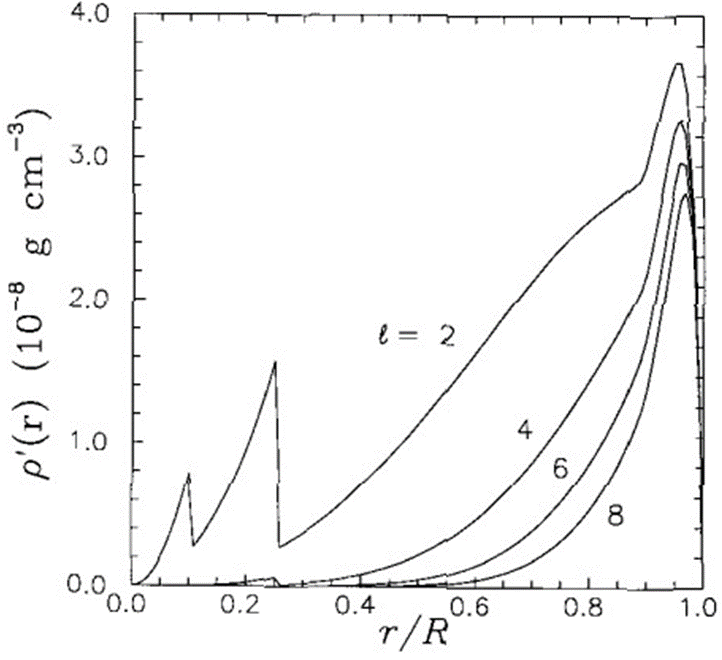
\includegraphics[width=0.5\textwidth]{marley_and_porco.png}
\caption{Density variation (perturbation) $\rho^{'}(r)$ versus scaled radial distance from the center to the surface of the planet \cite{Marley1993PlanetaryAM}.} \label{fig:my_label}
\end{figure}


Many gas giant models assume that amplitudes are smooth functions of frequencies, $l$ and $m$, as given in \cite{PMID:36042221}. This paper does an analysis of potential normal mode signals in Jupiter’s gravitational field, which could be comparable to the amplitudes of Saturnian normal-mode oscillations. In particular, for the figure extracted, the points marked $“f”$ on those plots are some of the same fundamental modes we are looking at in Saturn’s rings. Note the figure gives these signals in terms of zonal harmonic coefficients, which was gotten from potential amplitudes, through Juno spacecraft gravity measurements. Based on the results in \cite{PMID:36042221}, it is clearly evident that the normal-mode amplitudes for Jupiter varies increasingly, and smoothly, with decreasing angular degrees, $l$. Having a similar result for Saturn, and what such trends might look like, will pave the way for more understanding about its interior dynamics.
\begin{figure}[h] 
\centering
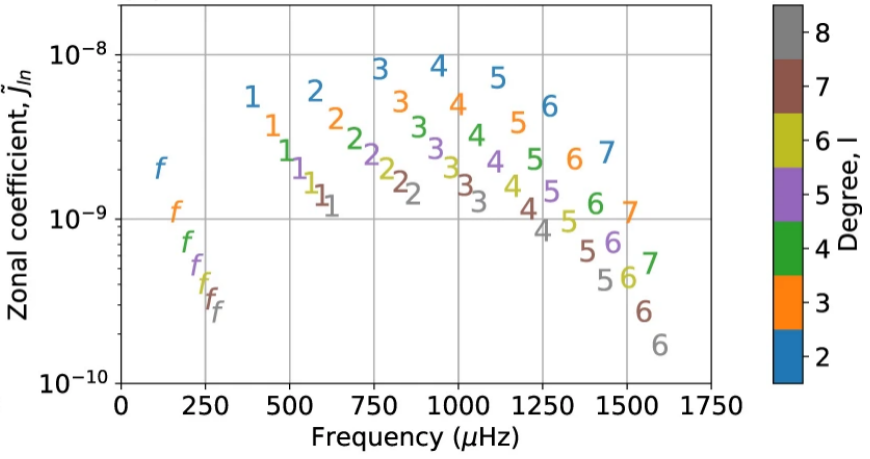
\includegraphics[width=0.6\textwidth]{durante.png}
\caption{The letters f and the numbers indicate, f-modes and the radial order of p-modes (up to n = 7) \cite{PMID:36042221}.} \label{fig:my_label}
\end{figure}

Finally, there are not yet measurements of individual planetary normal-mode amplitudes for Saturn. A catalogue of such measurements will assist with an accurate description of different excitation sources that could produce different signals at different values of oscillation frequencies, $l$ and $m$.

%from \cite{Marley1993PlanetaryAM},  similar research has been done at Jupiter, and the results show that, normal (fill in the blanks and attach diagrams/figures)...likewise, from \

Starting from the planet, and further out within the stretch of the C-ring, we aim to discuss the nature of Saturn's oscillatory phenomenon and how it initiates its effect across the particles located along the ring plane. We shall also lay the theoretical framework that explains the most profound phenomenon across the C-ring, the spiral density wave, as well as the corresponding normal-mode amplitudes responsible for the aforesaid phenomenon, which could serve as a link towards knowing what makes the planet ring (acoustically).

%........................................................................................................

\section{Background}
Saturnian oscillations, which are characterized by their fluid nature, are classified based on the types of displacements that occur during their propagation \cite{Marley1993PlanetaryAM}. In the case of stars and planets, nonradial oscillations can be further subdivided into three main categories: p-modes, g-modes, and f-modes. P-modes are associated with resonant acoustic disturbances, where the primary restoring force is pressure. Similarly, g-modes are linked to resonant internal gravitational disturbances, with gravity serving as the main restoring force. F-modes, also known as the fundamental mode, represent the fundamental oscillation mode observed in either p-modes or g-modes.


\subsection{Planetary Oscillations}
%..............................................................................................................
%The Saturnian oscillations, being fluidic in nature, are classified in terms of radial and nonradial displacements produced during propagation \cite{Marley1993PlanetaryAM}. Typically for stars and planets, there are basic subclasses of nonradial oscillations responsible for nonradial displacements during propagation: the p-modes, the g-modes, and the f-modes. The p-modes are synonymous with resonant acoustic disturbances whose dominant restoring force is pressure. Likewise, the g-modes are synonymous with resonant internal gravitational disturbances, with their dominant restoring force as gravity. The f-modes, an acronym for fundamental mode, is the basic mode of either the aforesaid p-mode or the g-mode.
%..............................................................................................................

Considering the largest perturbations to external gravitational field \cite{article} \cite{Marley1993PlanetaryAM}\cite{Mankovich_2019}, a Saturnian oscillation mode creates a density perturbation inside the planet, which in turn creates a time-dependent Eulerian perturbation to its bulk property (the mass density corresponding
to the $lmn$ normal mode in the planet) is expressed in terms of surface spherical harmonics, $Y_{l}^{m}(\theta,\phi)$ as: 
\begin{equation}
    \rho_{lmn}^{'}(r,\theta,\phi,t) =   \rho_{lmn}^{'}(r)Y_{l}^{m}(\theta,\phi)e^{-i\sigma_{lmn}t},
\end{equation}
$\sigma_{lmn}$ is the mode oscillation frequency in the corotating frame with the planet. $r$ is the radius, $\theta$ is the colatitude, and $\phi$ is the azimuth angle respectively. The surface spherical harmonics, $Y_{l}^{m}(\theta,\phi)$, is given in terms of the associated Legendre polynomials as: 
\begin{equation}
     Y_{l}^{m}(\theta,\phi) = (-1)^{(m+|m|)/2} \sqrt{\frac{(2l+1)}{4\pi}\frac{(l-|m|)!}{(l+|m|)!}}P^{m}_{l} (\cos\theta)e^{im\phi}
\end{equation}
$\forall$  $l \in [0, \infty)$ and $m \in [-l,+l]$.

Alternatively, we can express other properties of the planetary oscillations using similar description, for example the pressure, P, or the gravitational potential, $\Phi$, in place of the density, $\rho_{lmn}^{'}(r,\theta,\phi,t)$.

In the field of seismology, we generally describe an oscillation-mode in terms of three integers, namely l, m, and n. Projecting these integers on a spherical surface, the angular degree, $l$, measures the number of circles bounding the regions of positive and negative perturbations. The oscillation's azimuthal order, $|m|$ $(m = -l, -l+1, ..., 0,..., l-1, l)$, accounts for the number of great circles passing through the polar axis that form longitudinal boundaries. The quantity, $l-|m|$, accounts for the number of latitudinal circles forming latitudinal boundaries, while $2|m|$ accounts for zero crossings in the longitudinal direction. 

Furthermore, we can visualize the planetary oscillations using few simple properties of the spherical harmonic functions. When the angular order $m$ is zero, the harmonics are called zonal and oscillate only in the latitudinal direction. When $l=|m|$ the harmononic are called sectoral and oscillate only in the longitudinal direction.  For other values of $m$ the harmonics are called tesseral and oscillate in both the longitudinal and latitudinal directions. The equivalent Cartesian wavelength for a spherical harmonic function of degree $l$ is approximately given as, $\lambda = 2\pi R/\sqrt{l(l+1)}$. R is the radius of the sphere, and this result is known as the Jeans relation \cite{https://doi.org/10.1029/2018GC007529}.


Interestingly, when $l-m$ is even, such modes are symmetric about the equator and tend to produce periodic radial gravitational perturbations in the equatorial plane, which are responsible for driving spiral density waves in the rings. But when $l-m$ is odd, such modes are anti-symmetric and are located about the equator. They produce periodic vertical perturbations in the equatorial plane, and are responsible for driving bending waves in the rings. The third integer, n, accounts for the number of radial nodes in the mode's density profile, between the center of the planet and its surface \cite{FRENCH2021114660}. When $n=0$, the mode is referred to as the fundamental-mode (f-mode). Also, when $m>0$, these modes rotate in the same direction as the planet (prograde), while $m<0$ modes rotate in opposite direction to the planet (retrograde). 

So far, the detected signals used in this work involve mostly modes with $l\geq 2$, and no $l=0$ modes, since they are not liable to generate noticeable external gravitational perturbations. A similar case holds for the dipolar f-modes ($l=1$), that are liable to generate fictitious oscillation in Saturn's center of mass \cite{FRENCH2021114660}.






From \cite{Marley1993PlanetaryAM} \cite{FRENCH2021114660}, suggestions have been made that the internal oscillations most likely to be responsible for driving density waves in the rings would be f-modes with $l=|m|$, the sectoral modes. These suggestions have been found to be true, following reported OLD-type density waves in the C-ring, with results consistent within the expectation values \cite{Hedman_2013} \cite{10.1093/mnras/stu1503}. Another side to the previous results is the table showing the values for the mass estimates from the gravitational potentials, responsible for the spiral density wave amplitudes. The table clearly shows that none of these waves were excited by one or more of Saturn's moons, this implies that, most likely, the waves detected are as a result of planetary normal-mode oscillations (remember to add a diagram here).
\begin{figure}[h] 
\centering
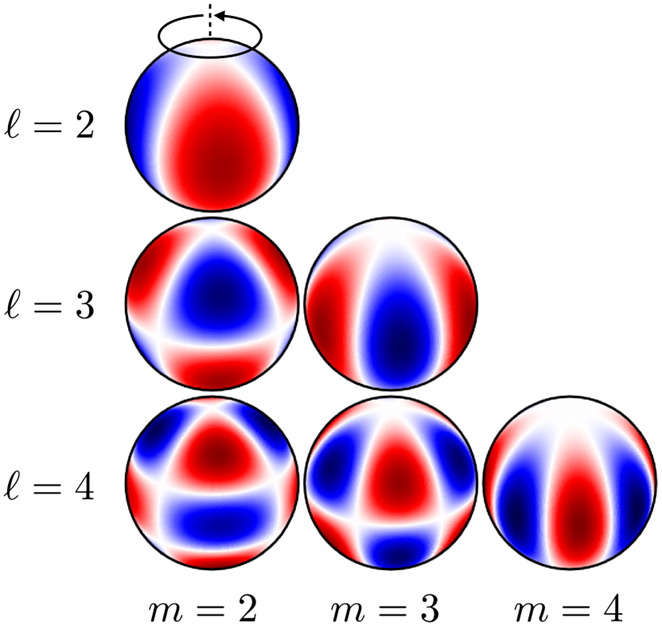
\includegraphics[width=0.5\textwidth]{mankovitch2.png}
\caption{A visual of some of the spherical harmonics relevant for Saturn ring seismology. $l$ denotes angular degree, while $m$ denotes azimuthal order \cite{Mankovich_2019}.  The color map corresponds to the magnitude of the density and gravity field perturbations, arising from oscillation. There is a downward trend of angular
degree ($l$) increase, and rightward increase in azimuthal order ($m$).} \label{fig:my_label}
\end{figure}

Understanding the aforesaid modes of oscillations help to clearly decipher the dynamics of this magnificent gas giant. Through the combination of observational data (Voyager and Cassini mostly) , theoretical models, and computer simulations, planetary scientists have been able to gain valuable insights into Saturn's internal structure, its atmospheric circulation, and the intricacies between its moons and the planet itself.

%So far, we are aware that the wave signals detected are not as a result of either one or more of Saturn's rings, based on measurements of mass estimates arising from the gravitational potentials of the wave signals detected, but as a result of the gravitational perturbations from Saturn (please see table below) .

%......Explain the process and attach equations where necessary...

%.............Add diagrams of different spherical harmonics for a sphere and use it to describe the acoustic oscillations of Saturn......



\subsection{Overview of Planetary Ring Seismology}

Planetary ring seismology is a field of study that uses the analysis of waves and vibrations within planetary rings to better understand their physical characteristics and formation history. By studying the way in which these waves propagate, researchers can gain insight into the density and composition of the particles within the rings, as well as the gravitational and tidal forces that influence their behavior.

On the other hand, planetary ring dynamics involves the study of the motion and behavior of particles within planetary rings. This could include the understanding of the gravitational, collisional, and electromagnetic forces that act on the particles, as well as the formation and evolution of the rings themselves.

By analyzing the distribution and behavior of the particles in a planetary ring, both areas of research can help provide researchers with more insight into the history and evolution of the planet and its moons. For example, the distribution of particles in Saturn's rings can provide information about the formation and evolution of Saturn's moon system. Also both fields could have implications for our understanding of planet formation and the evolution of planetary systems more broadly.


\subsection{Saturn’s C Ring}
Saturn's C ring is one of the most fascinating features of the sixth planet from the sun, spanning from about 74,658 km to 92,000 km from the planet's center, lying between the brighter B ring and the more diffuse D ring. The C Ring is made up of small particles ranging in size from micrometers to centimeters, and it is unique in that it has a peculiar wave-like pattern \cite{2009sfch.book..375C}\cite{Hedman_2018}\cite{Nicholson1990AnAR}. The waves across the C Ring were first observed by the Voyager spacecraft in the early 1980s. These waves are caused by gravitational interactions between the ring particles and Saturn's moons. As the moons pass by the ring, they create a gravitational disturbance that propagates through the ring in the form of a wave\cite{Hedman_2013}\cite{2014MNRAS.444.1369H}\cite{Hedman_2018}\cite{Marley1993PlanetaryAM}\cite{Nicholson1990AnAR}. These waves in the C Ring are incredibly precise, with wavelengths ranging from 30 to 180 kilometers. They are also very consistent, with the same patterns appearing year after year. The cause of this consistency is still not fully understood, but it is believed to be related to the structure of the ring particles themselves \cite{Hedman_2013}\cite{2014MNRAS.444.1369H}\cite{Hedman_2018}.

\begin{figure}[h] 
\centering
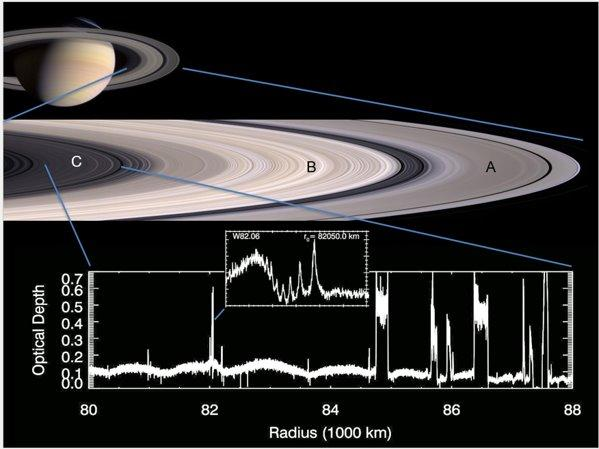
\includegraphics[width=0.7\textwidth]{Ring_Picture_Hedman_2018.jpg}
\caption{A picture of the A, B and C(Zoomed in) rings \cite{Hedman_2018}. An optical depth profile zoomed in on one of the waves (W82.06).} \label{fig:my_label}
\end{figure}



\subsection{Density Waves}
Spiral density and bending waves are well-researched and understood phenomena in the rings of Saturn, and they have provided valuable information about the surface mass density and viscosity of the main ring regions \cite{2009sfch.book..375C}\cite{Hedman_2013}\cite{2020AGUA....100142M}. The majority of these waves are caused by resonances with external satellites, especially in the A and B rings. However, another set of waves has been discovered in recent times, primarily in the C ring, which are not caused by satellites but by irregularities in Saturn's own gravitational field \cite{Hedman_2013}\cite{2014MNRAS.444.1369H}\cite{Hedman_2018}.Our focus is on studying the waves that are generated in Saturn's rings by the planetary normal modes. Specifically, we are exploring the inner C ring which has not been extensively researched before \cite{FRENCH2019599}\cite{Hedman_2013}. The waves in this area have very short wavelengths, which has posed a challenge for previous studies as they relied on precise calculations of wave phases to identify them \cite{FRENCH2019599}\cite{Hedman_2013}\cite{Hedman_2018}\cite{Tiscareno_2007}.In the next section, we aim to outline the basics of Fourier analysis and device an efficient algorithm for Fourier transformations, to use in processing Cassini's VIMS (Visual and Infrared Mapping Spectrograph) data, since other tested algorithms have resulted to an inefficient result. Thereafter, we will apply the new algorithm to our data and present the results achieved using this technique.




%\begin{figure}[h] 
%\centering
%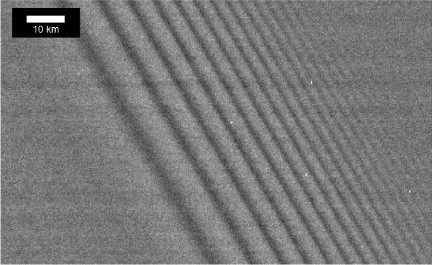
\includegraphics[width=0.7\textwidth]{Main_Wave_Web capture_3-4-2023_183537_reader.elsevier.com.jpeg}
%\caption{A portion of Cassini image N1467345975, showing the nearly-arche-typal Prometheus 9:8 [spiral] density wave \cite{Tiscareno_2007}.} \label{fig:my_label}
%\end{figure}
%................................................................................................................

\subsubsection{The Theory of Spiral Density Waves: Linear Density Wave Model}
In this section, we outline the concept of spiral density waves, how it is formed across Saturn's C ring and the mathematical representation of such phenomenon.
Basically, when normal-mode oscillations take place within gaseous planets, like Saturn, they do so in terms of vibrations, and these vibrations in turn give rise to variations in density within the planet, causing disturbances to be generated within the planet, and these disturbances in turn propagate towards the exterior of Saturn. Saturn's gravitational field simply couples these disturbances to the plane of the rings, and these disturbances travel across the stretch of the ring in form of density waves, spiral density and spiral bending waves. Our main focus is on the spiral density waves since their main cause are as a result of normal mode excitation within Saturn.


For a better understanding of this work on the spiral density wave analysis, we need to outline the theory behind the algorithms used in the subsequent sections.
Here, we are utilizing the density wave model to produce anticipated wave profiles \cite{Nicholson1990AnAR}. The specific model we are using is the linear, damped model which was originally derived and elaborately introduced by Shu in 1984 \cite{article}. To provide the essential details for our project, we will give a concise explanation of the model equations as well as the model parameters. This will help us to understand the workings of the model better and enable us to use it more effectively in our project. The linear, damped model is a well-established method that has been utilized in many scientific studies to describe a variety of astronomical phenomena.

%   EDITED SECTION NOVEMBER 2023. 
%   FULL DERIVATION FOR LINEAR DENSITY WAVEMODEL

Usually, when these waves are propagated across the ring, they are displayed as fluctuations in the density of the ring's surface, which affects its optical properties. This fluctuation has an m-fold symmetry and rotates with respect to the fixed reference frame at a rate of $\Omega_{p}$. The altered surface density distribution, normalized to the background density in areas outside the waves' region, $\sigma_{0}$, is represented by the expression \cite{Nicholson1990AnAR}:

\vspace{2pt}

\begin{equation}
\Delta \sigma(r,\lambda,t) = 1 + \Re\{-iA_{L}[\pi^{-1/2}-2i\xi H(\xi)]e^{i\phi}\}e^{-(\xi /\xi_{D})^{3}},
\end{equation}
The wave phase, $\phi$, and dimensionless distance from the resonance location, $\xi$, are clearly defined in the equations below, alongside $\xi_{D}$, which denotes the characteristic damping length of the wave. 

\vspace{2pt}
Simplifying the previous equation using Euler's identify, we have the variant below:
\begin{equation}
\Delta \sigma(r,\lambda,t) = 1 + \Re\{A_{L}e^{i(\phi-\pi/2)}[\pi^{-1/2}+2\xi e^{-i\pi/2}H(\xi)]\}e^{-(\xi/\xi_{D})^{3}}
\end{equation}

\vspace{2pt}

The function $H(\xi) = \pi^{-1/2}e^{-i\xi^{2}}\int_{-\infty}^{\xi}e^{i\eta^{2}}d\eta$. $H(\xi)$ includes the Standard Fresnel integral. Let $H(\xi) = \pi^{-1/2}e^{-i\xi^{2}}\gamma(\xi)$, so that the Standard Fresnel integral, $\gamma(\xi)$, is excluded from the function, $H(\xi)$. Thus we have the expression below:
\begin{equation}
    \gamma(\xi) = \int_{-\infty}^{\xi}e^{i\eta^{2}}d\eta
\end{equation}


Far into the region of wave propagation, $\xi$ is considered large and positive  \cite{Nicholson1990AnAR} \cite{1984prin.conf..513S}. Also considering the notion that the complex-Gaussian expression is exponentially convergent, we can simply separate the aforesaid integral for easy analysis resulting to the expression,
\begin{equation}
    \gamma(\xi) = \int_{-\infty}^{+ \infty}e^{i\eta^{2}}d\eta - \int_{\xi}^{\infty}e^{i\eta^{2}}d\eta = \gamma_{1} + \gamma_{2}
\end{equation}

\textbf{First Part of Integral:}
Here in this section, we are going to resolve the first part of the expanded integral for $\gamma(\xi)$, using contour integration. Let $\gamma_{1} = \int_{-\infty}^{+ \infty}e^{i\eta^{2}}d\eta$ and $\gamma_{2} = - \int_{\xi}^{\infty}e^{i\eta^{2}}d\eta$.

Considering $\gamma_{1}$, and since it is similar to the real Gaussian function, we devise a technique along the lines of Contour integration to bring it closer to the real Gaussian expression for easy analysis. Let,
\begin{equation}
    \gamma_{1} = \int_{-\infty}^{+ \infty}e^{i\eta^{2}}d\eta = 2\int_{0}^{+ \infty}e^{-(-i\eta^{2})}d\eta.
\end{equation}
Using polar coordinate expression for the arguments of $\gamma_{1}$, we have this as:
\begin{equation}
    \gamma_{1} = 2\int_{0}^{+ \infty}e^{-(e^{-i\pi/2} \eta^{2})}d\eta.
\end{equation}
We go on to factorize the previous equation and this results to, 
\begin{equation}
    \gamma_{1} = 2\int_{0}^{+ \infty}e^{-(e^{-i\pi/4} \eta)^{2}}d\eta.
\end{equation}
By substituting a variable for the exponential argument, we let $\rho = e^{-i\pi/4} \eta$ \cite{video}. Reshuffling the limits of our integral, we have: 
\begin{equation}
    \gamma_{1} = 2 e^{i\pi/4} \lim_{{R \to \infty}} \int_{0}^{Re^{-i\pi/4}} e^{-(\rho)^{2}} \, d\rho
\end{equation}

Let $\gamma_{1}^{'}$ represent the coefficient of 2 and the Euler argument in the main expression for $\gamma_{1}$, we have this as: $\gamma_{1}^{'} = \lim_{{R \to \infty}} \int_{0}^{Re^{-i\pi/4}} e^{-(\rho)^{2}} \, d\rho$, hence $\gamma_{1} = 2 e^{i\pi/4} \gamma_{1}^{'}$.

%............................................
\begin{figure}[h] 
\centering
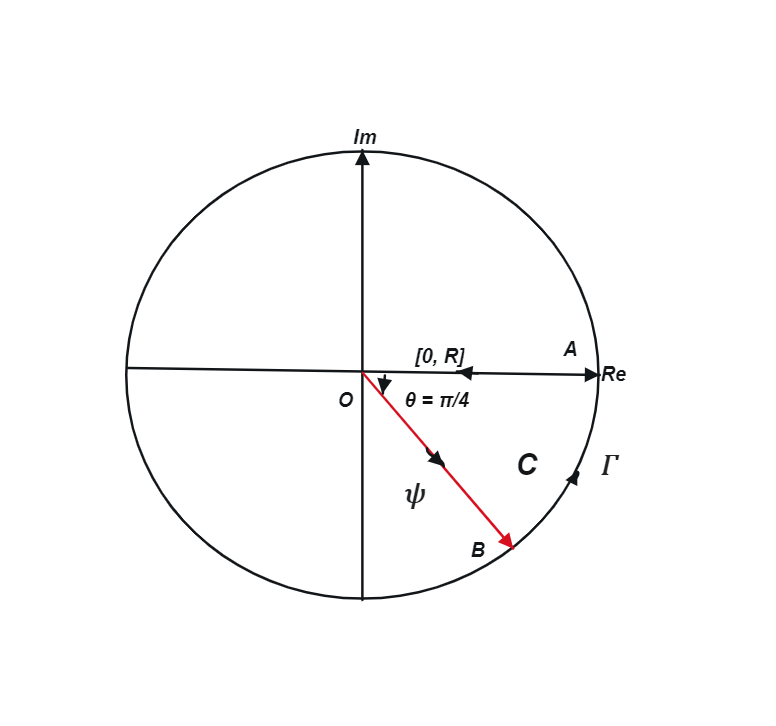
\includegraphics[width=0.8\textwidth]{COUNTOUR_INTEGRATION_DIAGRAM.png}
\caption{ Description of a pizza-shaped contour, consisting of the real (horizontal) and imaginary (vertical) axis.} \label{fig:my_label}
\end{figure}
%............................................

Considering the closed contour, as given in the diagram, for a pizza-shaped type of contour slice at an angle of $\pi/4$ radian (this angle also buttresses the asymptotic nature of $\xi$ \cite{Tiscareno_2007}), we can parametrize the previous expression and go on to evaluate the exact value of the Fresnel integral. This simply allows us to decomposed our contour integration according to the three sections present in our defined contour using complex analysis notations,
\begin{equation}
    \oint_{C} e^{-(z)^{2}} \, dz = \int_{\Psi} e^{-(z)^{2}} \, dz + \int_{\Gamma} e^{-(z)^{2}} \, dz + \int_{R}^{0} e^{-(z)^{2}} \, dz.
\end{equation}


Using Cauchy-Riemann's theorem, $\oint_{C} e^{-(z)^{2}} \, dz = 0$ (on the left hand side of the equation), since it is holomorphic inside and on $C$. Next, we consider the three sections of the given contour.

Given the conditions, $C = \left\{ z = x : 0 \leq x \leq R \right\} \cup \left\{ z : z = Re^{i\theta}, -\frac{\pi}{4} \leq \theta \leq 0 \right\} \cup \left\{ z : z = r,  0 \leq r \leq Re^{-i\frac{\pi}{4}}\right\}$, we can start with the line segment OB, $\Psi$. Here, 
\begin{equation}
    \int_{\Psi} e^{-(z)^{2}} \, dz = \int_{0}^{Re^{-i\frac{\pi}{4}}} e^{-(r)^{2}} \, dr.
\end{equation}
As $R \rightarrow \infty$, the integral along $\Psi$ assumes the format of a typical Gaussian integral, hence $\int_{0}^{\infty} e^{-(r)^{2}}\, dr = \frac{\sqrt{\pi}}{2}$.

Considering the arc BA, corresponding to the section $\Gamma$ of our contour integration,
\begin{equation}
    \int_{\Gamma} e^{-(z)^{2}} \, dz = \int_{-\frac{\pi}{4}}^{0} e^{-(z)^{2}} \, dz, \hspace{3pt} dz = iRe^{i\theta} d \theta. 
\end{equation}
By substitution we have the form for $\Gamma$ as,
\begin{equation}
    \int_{\Gamma} e^{-(z)^{2}} \, dz = \int_{-\frac{\pi}{4}}^{0} e^{-R^{2}e^{2i\theta}} iRe^{i\theta} d\theta. 
\end{equation}
Considering the absolute value of the given integral along the arc, $\Gamma$, this can be written as:
\begin{equation}
   \left| \int_{\Gamma} \right| \leq \int_{-\frac{\pi}{4}}^{0} \left|e^{-R^{2}e^{2i\theta}} iRe^{i\theta}\right| d\theta = R\int_{-\frac{\pi}{4}}^{0} \left|e^{-R^{2}e^{2i\theta}}\right| d\theta = R\int_{-\frac{\pi}{4}}^{0} \left|e^{-R^{2}[{\cos{(2\theta)} + i\sin{(2\theta)}}]}\right| d\theta.
\end{equation}
Using Euler's indentity, we reduce the expression to its real part only,
\begin{equation}
   \left| \int_{\Gamma} \right| \leq R\int_{-\frac{\pi}{4}}^{0}e^{-R^{2}\cos(2\theta)}d\theta.
\end{equation}
Intuitively, an integral like the one above with such property, vanishes as R becomes large. We are going to validate this claim analytically. A plot of $\cos(2\theta)$ $\forall \theta \in [-\frac{\pi}{4}, 0]$ simply shows that it has its minimum point at $-\frac{\pi}{4}$ and maximum point at $0$. We actually need a function within the same bound that best maximizes the $\cos(2\theta)$ within the exponential argument, to help validate our claim. An optimized function for this operation is $f(\theta) = \frac{4\theta}{\pi}+1$. This implies that, $\cos(2\theta) \geq f(\theta), \forall \theta \in [-\frac{\pi}{4}, 0]$.
Therefore, $e^{-R^{2}\cos(2\theta)} \leq e^{-R^{2}(\frac{4\theta}{\pi}+1)}$. Applying this to the previous case, 
\begin{equation}
   \left| \int_{\Gamma} \right| \leq R\int_{-\frac{\pi}{4}}^{0}e^{-R^{2}(\frac{4\theta}{\pi}+1)}d\theta = \frac{\pi}{4R}(1 - e^{-R^{2}})
\end{equation}
So we establish that, 
\begin{equation}
\lim_{{R \to \infty}} \left| \int_{\Gamma} \right| = \lim_{{R \to \infty}} \frac{\pi}{4R}(1 - e^{-R^{2}}) \leq 0.
\end{equation}

Next, we consider line segment OA, the real part of the contour. Redirecting the integral expression for that section, we have:
\begin{equation}
 \lim_{{R \to \infty}} \int_{R}^{0} e^{-(z)^{2}} \, dz = \lim_{{R \to \infty}} - \int_{0}^{R} e^{-(x)^{2}} \, dx = - \int_{0}^{\infty} e^{-(x)^{2}} \, dx = -\frac{\sqrt{\pi}}{2}.
\end{equation}

Recall, $\oint_{C} e^{-(z)^{2}} \, dz = \int_{\Psi} e^{-(z)^{2}} \, dz + \int_{\Gamma} e^{-(z)^{2}} \, dz + \int_{R}^{0} e^{-(z)^{2}} \, dz.$ Using the answers to each integral, $0 = \frac{\sqrt{\pi}}{2} + 0 - \frac{\sqrt{\pi}}{2}$, which is \textbf{true}. This shows that, $\gamma_{1}^{'} = \frac{\sqrt{\pi}}{2}$ and $\gamma_{1} = \sqrt{\pi}e^{i\pi/4}$.

\vspace{3pt}

\textbf{Second Part of Integral:}
For the case of $\gamma_{1}$, we could decompose it into a standard Fresnel integral and an integral that behaves like a Fresnel function as its argument approaches infinity. Here,
\begin{equation}
\gamma_{2} = - \int_{\xi}^{\infty}e^{i\eta^{2}}d\eta = -\int_{0}^{\infty}e^{i\eta^{2}}d\eta + \int_{0}^{\xi}e^{i\eta^{2}}d\eta = -\frac{\sqrt{\pi}}{2}e^{i\frac{\pi}{4}} + \int_{0}^{\xi}e^{i\eta^{2}}d\eta.
\end{equation}
Using the de Moivre's theorem, $\int_{0}^{\xi}e^{i\eta^{2}}d\eta = \int_{0}^{\xi}[cos(\eta^{2}) + isin(\eta^{2})]d\eta$. Let $C(\xi) = \int_{0}^{\xi}\cos(\eta^{2})d\eta$ and $S(\xi) =  \int_{0}^{\xi}\sin(\eta^{2})d\eta$ assume the real and imaginary parts of the asymptotic Fresnel expressions, respectively, so that $\int_{0}^{\xi}e^{i\eta^{2}}d\eta = C(\xi) + iS(\xi)$.

\vspace{5pt}

We can express the asymptotic behaviour of the aforesaid Fresnel integrals using the given forms as \cite{abramowitz1968handbook}\cite{enwiki:1181389148}\cite{wolfram-alpha-notebook}: 
\begin{equation}
    C(\xi) = \sqrt{\frac{\pi}{8}}\,\text{sgn}(\xi) + \left[1 + O\left(\xi^{-4}\right)\right]\left(\sin(\xi^2)\left(\frac{1}{2\xi}\right) + \cos(\xi^2)\left(-\frac{1}{4}\,O\left(\xi^{-3}\right)\right)\right)
\end{equation}
and
\begin{equation}
   S(\xi) = \sqrt{\frac{\pi}{8}}\,\text{sgn}(\xi) - \left[1 + O\left(\xi^{-4}\right)\right]\left(\cos(\xi^2)\left(\frac{1}{2\xi}\right) + \sin(\xi^2)\left(\frac{1}{4}\,O\left(\xi^{-3}\right)\right)\right).
\end{equation}


In the case of our model, we assume a moderate propagation of the density waves, which implies that as $\xi \rightarrow \infty$, $\mathcal{O}(\xi^{-n}) \rightarrow 0$ $\forall$ $n>1$. The moderated expression for the Fresnel integrals becomes, 
\begin{equation}
\int_{0}^{\xi}e^{i\eta^{2}}d\eta = \sqrt{\frac{\pi}{8}}\,\text{sgn}(\xi) + \frac{\sin(\xi^2)}{2\xi} + i\left(\sqrt{\frac{\pi}{8}}\,\text{sgn}(\xi) - \frac{\cos(\xi^2)}{2\xi}\right) = \frac{1}{2}\left[\sqrt{\pi}e^{i\frac{\pi}{4}}\,\text{sgn}(\xi) - \frac{i}{\xi}e^{i\xi^{2}}\right].
\end{equation}
Therefore, 
\begin{equation}
\gamma_{2} = \frac{\sqrt{\pi}}{2}e^{i\frac{\pi}{4}}\left[\,\text{sgn}(\xi) - 1\right] + \frac{e^{i(\xi^{2} - \pi/2)}}{2\xi},
\end{equation}
so that $\gamma(\xi) = \frac{\sqrt{\pi}}{2}e^{i\frac{\pi}{4}}\left[\,\text{sgn}(\xi) + 1\right] + \frac{e^{i(\xi^{2} - \pi/2)}}{2\xi}$.

Now, we re-express  $H(\xi)$ as follows, 
\begin{equation}
    H(\xi) = \frac{e^{i(\frac{\pi}{4} - \xi^{2})}}{2}\left[\,\text{sgn}(\xi) + 1\right] + \frac{e^{i(-\pi/2)}}{2\xi \sqrt{\pi}}
\end{equation}

Considering the linear density wave equation, $\Delta \sigma(r,\lambda,t)$, this becomes:
\begin{equation}
 \Delta \sigma(r,\lambda,t) = 1 + \Re\{A_{L}e^{i(\phi-\pi/2)}[\pi^{-1/2} + \xi e^{-i{(\pi/4 + \xi^{2})}}\left[\,\text{sgn}(\xi) + 1\right] + \pi^{-1/2}e^{-i\pi}]\} e^{-(\xi/\xi_{D})^{3}}
\end{equation}

\begin{equation}
\Delta \sigma(r,\lambda,t) = 1 + \Re\{A_{L}e^{i(\phi-\pi/2)}[\xi e^{-i{(\pi/4 + \xi^{2})}}\left[\,\text{sgn}(\xi) + 1\right]]\} e^{-(\xi/\xi_{D})^{3}}
\end{equation}


\begin{equation}
\Delta \sigma(r,\lambda,t) = 1 + \Re\{A_{L}[\xi e^{i{(\phi - 3\pi/4 - \xi^{2})}}\left[\,\text{sgn}(\xi) + 1\right]]\} e^{-(\xi/\xi_{D})^{3}}
\end{equation}

Using the de Moivre's theorem as well as the real part of the linear density wave equation, this expression becomes as:
\begin{equation}
\Delta \sigma(r,\lambda,t) = 1 + {\{A_{L}\xi\left[\,\text{sgn}(\xi) + 1\right]\cos{(\phi - 3\pi/4 - \xi^{2})}}\}e^{-(\xi/\xi_{D})^{3}}
\end{equation}


Removing the "unit" vertical translation, and considering both directions of wave propagations, this results to the given expression: 
\begin{equation}
   \Delta \sigma(r,\lambda,t) = A_{L}\xi\\e^{-\left(\frac{\xi_{*}}{\xi_{D}}\right)^3}\cos\left(\phi-\frac{3\pi}{4}-\xi^2\right)\zeta(\xi_{*})
\end{equation}

Where $\zeta(\xi_{*})$ encompases a generalized signum function, $\zeta(\xi_{*}) = [1 + \mathrm{sgn}(m)\mathrm{sgn}(\xi)]$  and $ \mathrm{sgn}(\xi) = \left\{ \begin{array}{rcl}
1 & \forall
& \xi>0 \\ 0 & \forall & \xi=0 \\ -1 & \forall & \xi<0 \\
\end{array}\right\}$.

\vspace{3pt}

Here, $\sigma(r,\lambda,t)$ is the perturbed surface density distribution of the ring section, $r$ is the distance (in kilometers) away from the center of the planet, $\lambda$ and $t$ are the longitude and time of observation, respectively. $A_{L}$ is the dimensionless amplitude factor, it is dependent on the mass of the perturbing moon, inducing the wave \cite{Tiscareno_2007}. $\phi = m(\lambda_{s}(0)+\Omega_{s}t-\lambda$) is the wave phase; $\lambda_{s}(0)$ is the mean longitude of the satellite at $t=0$ and $\Omega_{s}$ is the orbital mean motion of the satellite. $\xi_{D}$ is the dimensionless damping parameter, which depicts the location at which the wave's amplitude ceases to grow and begins to decay. It is also sensitive to the viscosity of the ring \cite{Tiscareno_2007}.
From \cite{Nicholson1990AnAR} \cite{1984prin.conf..513S}, $\xi$ is a dimensionless quantity that specifies the distance from the resonant radius, $r_{L}$, and it is given as:
\begin{equation}
\xi = \left[\frac{3|m-1|\Omega_{L}^{2}r_{L}}{4\pi G \sigma_{0}}\right]^{\frac{1}{2}}\left(\frac{r-r_{L}}{r_{L}}\right), 
\end{equation}
and $\xi_{*} = \xi \mathrm{sgn}(r - r_{L})$.

\vspace{3pt}

The resonant radius, $r_{L}$, fixes the wave against translation in the radial direction \cite{Tiscareno_2007}. Similarly, the background surface density, $\sigma_{0}$, controls the rate at which the wavenumber increases with respect to the wave's distance from its resonant location \cite{Tiscareno_2007}. G is the Newtonian gravitational constant equivalent, in SI units, to 6.674 $\times 10^{-11} m^{3}kg^{-1}⋅s^{-2}$.
\textbf{Note:} $\zeta(\xi)$ is the general parameter used to account for spiral density waves with both positive and negative azimuthal orders, and such cases determine whether the sign of $\xi$ will either be positive or negative. We explain this in the wave-fitting routine.

\begin{figure}[h] 
\centering 
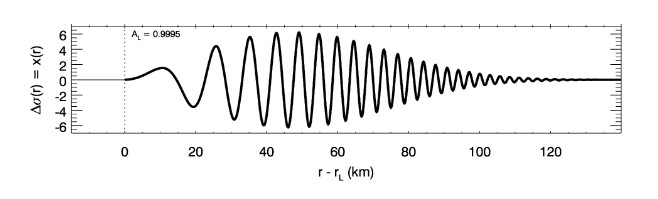
\includegraphics[width=1.0\textwidth]{Linear_Density_WM.jpg}
\caption{Synthetic density-wave radial profile generated by Equation (1) for a case of $m>0$ (prograde) \cite{Tiscareno_2007}.} \label{fig:my_label}
\end{figure}

%................................................................

%................................................................

%Usually, when these waves are propagated across the ring, they are displayed as fluctuations in the density of the ring's surface, which affects its optical properties. This fluctuation has an m-fold symmetry and rotates with respect to the fixed reference frame at a rate of $\Omega_{p}$. The altered surface density distribution, normalized to the background density in areas outside the waves' region, $\sigma_{0}$, is represented by the expression \cite{Nicholson1990AnAR}:

%\vspace{2}

%\begin{equation}
%\Delta \sigma(r,\lambda,t) = 1 + \Re\{A_{L}e^{i(\phi-\pi/2)}[\pi^{-1/2}+2\xi e^{-i\pi/2}H(\xi)]\}e^{-(\xi_{*} /\xi_{D})^{3}}
%\end{equation}

%\vspace{2}

%The function $H(\xi) = \pi^{-1/2}e^{-i\xi^{2}}\int_{-\infty}^{\xi}e^{i\eta^{2}}d\eta$. $H(\xi)$ includes the Standard Fresnel integral. Let $H(\xi) = \pi^{-\pi/2}e^{-i\xi^{2}}\gamma(\xi)$, so that $\gamma(\xi) = \int_{-\infty}^{\xi}e^{i\eta^{2}}d\eta$. Far into the region of wave propagation, $\xi$ is considered large and positive \cite{article}, resulting to the expression,
%\begin{equation}
 %   \gamma(\xi) = \int_{-\infty}^{+ \infty}e^{i\eta^{2}}d\eta - \int_{-\xi}^{\infty}e^{i\eta^{2}}d\eta = \frac{\sqrt{\pi}}{2}e^{i\pi/4} + \int_{0}^{\xi}e^{i\eta^{2}}d\eta.
%\end{equation}
%The first term was estimated using Cauchy-Riemann's integral formula alongside Jordan's Lemma, specifically for a pizza-shaped type of contour slice at an angle of $\pi/4$ radian (this angle also buttresses the asymptotic nature of $\xi$ \cite{Tiscareno_2007}). 

%\vspace{5}

%From \cite{abramowitz1968handbook}, $\int_{0}^{\xi}e^{i\eta^{2}}d\eta = \int_{0}^{\xi}\cos(\eta^{2})d\eta + i \int_{0}^{\xi}\sin(\eta^{2})d\eta = C(\xi) + i  S(\xi)$. $C(\xi)$ and $S(\xi)$ are the Fresnel integrals. As $\xi \rightarrow \infty$, $\mathcal{O}(\xi^{-n}) \rightarrow 0$ $\forall$ $n>1$. Thus: 
%$C(\xi) = \sqrt{\frac{\pi}{8}}sgn(\xi) + \frac{\sin(\xi^{2})}{2\xi}$ and $S(\xi) = \sqrt{\frac{\pi}{8}}sgn(\xi) - \frac{\cos(\xi^{2})}{2\xi}$. By substituting into the Fresnel integral and simplifying for a general case of positive azimuthal orders of the spiral density waves: 
%\begin{equation}
%\gamma(\xi) \approx \frac{\sqrt{\pi}}{2}[1 + sgn(\xi)]e^{i \pi/4} + \frac{e^{i(\xi^{2} - \pi/2)}}{2\xi}
%\end{equation}

%Finally, we put $H(\xi)$ into equation (1), and take the real part of the expression (neglecting the vertical translation). This results to the given expression: 
%\begin{equation}
 %   \Delta \sigma(r,\lambda,t) = A_{L}\xi\\e^{-\left(\frac{\xi_{*}}{\xi_{D}}\right)^3}\cos\left[\phi-\frac{3\pi}{4}-\xi^2\right]\zeta(\xi)
%\end{equation}

%Where $\zeta(\xi)$ encompases a generalized signum function, $\zeta(\xi) = [1 + \mathrm{sgn}(\xi)]$  and $ \mathrm{sgn}(\xi) = \left\{ \begin{array}{rcl}
%1 & \forall
%& \xi>0 \\ 0 & \forall & \xi=0 \\ -1 & \forall & \xi<0 \\
%\end{array}\right\}$.

%\vspace{3}

%Here, $\sigma(r,\lambda,t)$ is the perturbed surface density distribution of the ring section, $r$ is the distance (in kilometers) away from the center of the planet, $\lambda$ and $t$ are the longitude and time of observation, respectively. $A_{L}$ is the dimensionless amplitude factor, it is dependent on the mass of the perturbing moon, inducing the wave \cite{Tiscareno_2007}. $\phi = m(\lambda_{s}(0)+\Omega_{s}t-\lambda$) is the wave phase; $\lambda_{s}(0)$ is the mean longitude of the satellite at $t=0$ and $\Omega_{s}$ is the orbital mean motion of the satellite. $\xi_{D}$ is the dimensionless damping parameter, which depicts the location at which the wave's amplitude ceases to grow and begins to decay. It is also sensitive to the viscosity of the ring \cite{Tiscareno_2007}.
%From \cite{Nicholson1990AnAR} \cite{1984prin.conf..513S}, $\xi$ is a dimensionless quantity that specifies the distance from the resonant radius, $r_{L}$, and it is given as:
%\begin{equation}
%\xi = \left[\frac{3|m-1|\Omega_{L}^{2}r_{L}}{4\pi G \sigma_{0}}\right]^{\frac{1}{2}}\left(\frac{r-r_{L}}{r_{L}}\right), 
%\end{equation}
%and $\xi_{*} = \xi \mathrm{sgn}(r - r_{L})$.

%\vspace{3}

%The resonant radius, $r_{L}$, fixes the wave against translation in the radial direction \cite{Tiscareno_2007}. Similarly, the background surface density, $\sigma_{0}$, controls the rate at which the wavenumber increases with respect to the wave's distance from its resonant location \cite{Tiscareno_2007}. G is the Newtonian gravitational constant equivalent, in SI units, to $6.674 \times 10^{-11} m^{3}⋅kg^{-1}⋅s^{-2}$.
%\textbf{Note:} $\zeta(\xi)$ is the general parameter used to account for spiral density waves with both positive and negative azimuthal orders, and such cases determine whether the sign of $\xi$ will either be positive or negative. We explain this in the wave-fitting routine.

%\begin{figure}[h] 
%\centering 
%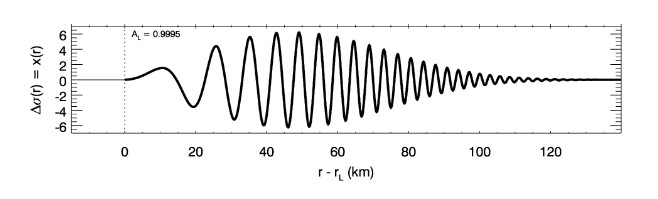
\includegraphics[width=1.0\textwidth]{Linear_Density_WM.jpg}
%\caption{Synthetic density-wave radial profile generated by Equation (1) for a case of $m>0$ (prograde) \cite{Tiscareno_2007}.} \label{fig:my_label}
%\end{figure}

%.................................................................
%.................................................................

\section{Methodology}
Having established the fundamental theoretical foundation for planetary oscillations and the associated effects across Saturn's (C)-ring(s), spiral density waves, our subsequent aim is to reinforce the mathematical tools employed in computing the necessary amplitudes of normal modes for Saturnian oscillations. The components of this toolbox are crucial in facilitating a precise and rigorous examination of the complex dynamics exhibited by spiral density waves, encompassing their periodic structures and frequencies.

\subsection{Wavelet Analysis}
 The method of Fourier transform provides us with valuable insights into the underlying physical properties of waves, which can be essential for understanding their behavior and predicting their future evolution. Ultimately, our application and interpretation of Fourier transform algorithms will help to shed light on the complex nature of spiral density waves and how they are excited from Saturn's interior.
 
Wavelet analysis is a method of time-frequency analysis that is scale independent and can provide more detailed information about the dominant frequencies present in a signal than traditional Fourier analysis. This is because wavelets can adapt to the local features of the signal at different scales, allowing for a more accurate representation of the signal's frequency content. In contrast, traditional Fourier analysis assumes a fixed window size, which can lead to inaccuracies in the frequency estimation of signals with non-stationary or time-varying properties. Thus, for signals with a wide range of dominant frequencies or non-stationary properties, wavelet analysis is often a more appropriate method of analysis \cite{APracticalGuidetoWaveletAnalysis}.

\subsubsection{Continous Wavelet Transform}
Assuming our unprocessed wave signal is given as $x(t)$. From \cite{mertins1999signal}\cite{pereyra2012harmonic}, we use a normalized wavelet $\psi \in L^2(\mathbb{R})$, having zero average, with shifting and rescaling parameters $b$ and $a$, respectively:
\begin{equation} 
\psi_{a,b}(t) = \frac{1}{\sqrt{|a|}} \psi\left(\frac{t-b}{a}\right)
\end{equation}
The Continous Wavelet Transformation derivable from our signal, $x(t)$, is given as:
\begin{equation} 
X_{w}(a,b) = \langle x, \psi_{a,b} \rangle =\int_{-\infty}^{+\infty} x(t) \psi_{a,b}^{*}(t) \, dt
\end{equation}
Here, $\psi_{a,b}^{*}(t)$ is the complex conjugate of $\psi_{a,b}(t)$. We can rewrite equation 4 as: $X_{w}(a,b) = \frac{1}{\sqrt{|a|}}\int_{-\infty}^{+\infty} x(t) \bar{\psi}\left(\frac{t-b}{a}\right) dt$ and let $\tilde{X}_{w}(a,b)=\int_{-\infty}^{+\infty} x(t) \bar{\psi}\left(\frac{t-b}{a}\right) dt$. Then our new equation 4 becomes: $X_{w}(a,b)=\frac{1}{\sqrt{|a|}}\tilde{X}_{w}(a,b)$. 
Here, the prefactor $\frac{1}{\sqrt{|a|}}$ is introduced in order to ensure that all scaled functions with $a\in\mathbb{R}$ have the same energy \cite{mertins1999signal}\cite{Roy_2022}\cite{APracticalGuidetoWaveletAnalysis}. Note also that $b\in\mathbb{R}$.







\subsubsection{Choice of Wavelet Function}
An efficient example of a normalized wavelet function that is “admissible”, has zero mean and is localized in both time and frequency space is the Morlet wavelet, comprising a plane wave modulated by a Gaussian \cite{doi:10.1146/annurev.fl.24.010192.002143}\cite{mertins1999signal}\cite{APracticalGuidetoWaveletAnalysis} and give as:
\begin{equation} 
\psi(t)= \pi^{-1/4}e^{i\omega_{0}t}e^{-t^2/2}
\end{equation}
where $\omega_{0}=6$, a dimensionless frequency which satisfies the admissibility condition \cite{doi:10.1146/annurev.fl.24.010192.002143}\cite{mertins1999signal}\cite{APracticalGuidetoWaveletAnalysis}.

\begin{figure}[h] 
\centering
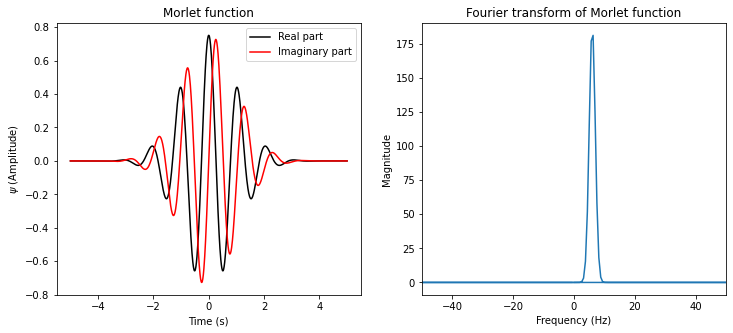
\includegraphics[width=0.8\textwidth]{Morlet_Plot_Python.png}
\caption{ Morlet function in time (real and imaginary) and frequency space.} \label{fig:my_label}
\end{figure}

It is worthy of note that, the Morlet wavelet does not have compact support but has exponential decay. This means that the wavelet function does not go to zero outside a certain range of values, but instead decays exponentially. Regarding the differentiability of the Morlet wavelet, it is not infinitely differentiable. No wavelet with finite support can be infinitely differentiable. This is because, for a wavelet to have compact support, it must be zero outside a certain interval. However, if a function is zero outside an interval, then it cannot have nonzero derivatives of all orders.

Finally, the Morlet wavelet does not come from an MRA (multiresolution analysis). This means that the Morlet wavelet cannot be generated by a series of dilations and translations of a single wavelet function, which is a key feature of MRAs. However, the Morlet wavelet can still be used in wavelet analysis for certain applications, like in our case.



\subsubsection{Phase-Correction in Fourier Space}
After transforming our signal profile into the required wavelet, we can assume a resulting complex wavelet profile in Fourier space as \cite{Hedman_2018}, 
\begin{equation}
    \tilde{X}_{w,i}(a,b) = \Gamma_{i}e^{i\Phi_{i}},
\end{equation}
where $\tilde{X}_{w,i}(a,b)$ is the complex phase-dependent wavelet transformation, $\Gamma_{i}$ is the complex amplitude, $\Phi_{i}$ is the wavelet phase which could be expressed as, $\Phi_{i} = \phi_{r}(r) + |m|(\lambda - \Omega_{p}t) + \phi_{0}$. $\phi_{r}(r)$ is the radiallly dependent portion of the wave-sphase, and for large distances from the resonant radius we can express it as \cite{1984prin.conf..513S},
\begin{equation}
    \phi_{r}(r) = \frac{3|m-1|M_{P}(r - r_{L})^{2}}{4\pi\sigma_{0}r^{4}_{L}}.
\end{equation}
All other parameters maintaining their usual meanings.   

For discrete observations of the longitude $\lambda_{i}$ and epoch time $t_{i}$, the phase parameter can be estmated using the discrete interpretation, $\phi_{i} = |m|[\lambda_{i} - \Omega_{p}t_{i}]$, given specific values of $|m|$ and $\Omega_{p}$. Given a specific wave with defined parameters, the required phase difference becomes $\Phi_{i} - \phi_{i} = \phi_{r}(r) + \phi_{0}$ for all occultations present. Now, the previous steps enables us to redefine the phase corrected wavelet as:
\begin{equation}
    \tilde{X}_{w,\phi,i}(a,b) = \tilde{X}_{w,i}(a,b)e^{i\Phi_{i}} = \Gamma_{i}e^{i(\Phi_{i} - \phi_{i})}.
\end{equation}

Given particular signals with m and $\Omega_{p}$ values, by implication of the phase correction, there will be the same phase for all the occulation profiles present, leading to an average non-zero phase-corrected wavelet:
\begin{equation}
    \langle\tilde{X}_{w,\phi}(a,b)\rangle = \frac{1}{N} \sum_{i=1}^{N}\tilde{X}_{w,\phi,i}(a,b).
\end{equation}

Any signal without similar phase attributes will average to zero, leaving the desired signal in the power of the average phase-corrected wavelet, expressed as,
\begin{equation}
    \mathcal{P}_{\phi}(r,k) = |\langle\tilde{X}_{w,\phi}(a,b)\rangle|^{2} = \left|\frac{1}{N} \sum_{i=1}^{N}\tilde{X}_{w,\phi,i}(a,b)\right|^{2}.
\end{equation}
On the other hand, all other signals will be captured in the average wavelet power,
\begin{equation}
     \bar{\mathcal{P}}(r,k) = \langle|\tilde{X}_{w,\phi}(a,b)|^{2}\rangle = \frac{1}{N} \sum_{i=1}^{N}|\tilde{X}_{w,\phi,i}(a,b)|^{2}.
\end{equation}

To guage how much of the signal is consistent with the assumed m and $\Omega_{p}$, we take the ratio \cite{Hedman_2013}:  $\mathcal{T}_{\phi}(r,k) = \frac{\mathcal{P}_{\phi}(r,k)}{\bar{\mathcal{P}}(r,k)}$ $\forall$ $\mathcal{T}_{\phi}(r,k) \in (0,1)$.








\subsubsection{Wavelet Reconstruction Formula}
For proper reconstruction, we use the average phase-corrected wavelet to create a reconstructed profile with given m, and pattern speed. 

We start by assuming $x_{\phi}\in L^2(\mathbb{R})$, we can reconstruct our signal using the famous Calderon's technique \cite{Caldern1964IntermediateSA}\cite{pereyra2012harmonic}\cite{Roy_2022}\cite{APracticalGuidetoWaveletAnalysis}:
\begin{equation}
x_{\phi}(t) = \frac{1}{C_{\psi}} \int_{0}^{\infty} \int_{-\infty}^{\infty} X_{w,\phi}(a,b) \frac{1}{|a|^{1/2}} \psi\left(\frac{t-b}{a}\right) \frac{db \, da}{a^{2}},
\end{equation}
provided $\psi(t)$ satisfies Calderón's admissibility condition \cite{Caldern1964IntermediateSA}: $C_{\psi} := \int_{-\infty}^{\infty} \frac{|\tilde{\psi}(\xi)|^2}{|\xi|} d\xi < \infty$ and must have a finite energy\cite{Roy_2022}\cite{APracticalGuidetoWaveletAnalysis}: $E_{\psi} = \int_{-\infty}^{\infty} |\psi(t)|^2 dt < \infty$. Here, $\tilde\psi(\omega)$ is the Fourier transform of $\psi(t)$, $\omega = 2\pi \mathcal{\beta}$ is the angular frequency, and $C_{\psi}$ is the admissibility constant. The above condition implies that $\tilde\psi(\omega)$ approaches zero faster than $\omega$ and must not have zero frequency component, $\tilde\psi(0)=0$ \cite{Roy_2022}.






\subsubsection{Alternative Wavelet function}
Recall, $X_{w,\phi}(a,b)=\frac{1}{\sqrt{|a|}}\tilde{X}_{w,\phi}(a,b)$. By direct substitution into equation 5, we have:
\begin{equation} 
x_{\phi}(t) = \frac{1}{C_{\psi}} \int_{0}^{\infty} \int_{-\infty}^{\infty}\frac{\tilde{X}_{w,\phi}(a,b)}{|a|} \psi\left(\frac{t-b}{a}\right) \frac{db \, da}{a^{2}}.
\end{equation}


We can also choose a completely different wavelet function, Morlet's technique, like the Dirac-delta function $\delta\left(\frac{b-t}{a}\right)$, instead of the analysing wavelet \cite{doi:10.1146/annurev.fl.24.010192.002143}\cite{Roy_2022}. Here: 
\begin{equation}
    x_{\phi}(t) = \frac{1}{C_{\psi}} \int_{0}^{\infty}\frac{1}{|a|} \left(\int_{-\infty}^{\infty} \tilde{X}_{w,\phi}(a,b)\delta\left(\frac{t-b}{a}\right)db\right)\frac{da}{a^2}
\end{equation}


Recall for a Delta function, $\delta(-x)=\delta(x)$ and $\int_{-\infty}^{\infty}\delta(x-d)f(x) dx=f(d)$.

Using $b=ay$, and working through the double-integral, we have: $\int_{-\infty}^{\infty} \tilde{X}_{w,\phi}(a,b)\delta\left(\frac{t-b}{a}\right)db = a\tilde{X}_{w,\phi}(a,t)$.

By direct substitution into equation 5, we arrive at a simplified single integral for our wavelet reconstruction given as \cite{doi:10.1146/annurev.fl.24.010192.002143}\cite{Roy_2022}\cite{APracticalGuidetoWaveletAnalysis}:
\begin{equation}
     x_{\phi}(t) = \frac{1}{C_{\delta}} \int_{0}^{\infty}\frac{\tilde{X}_{w,\phi}(a,t)}{|a|}\frac{da}{a}.
\end{equation}
Note: $C_{\psi}=C_{\delta}$, since we reconstructed the Fourier transforms using a Dirac delta function \cite{APracticalGuidetoWaveletAnalysis}.

\subsubsection{Choice of Scale: From Dyadic to Linear Scale}
Since we are working with nonorthogonal wavelet analysis, it is recommendable to use an arbitrary set of scale to build a more complete wavelet reconstruction formula for previous step above \cite{APracticalGuidetoWaveletAnalysis}. To enable us succeed in this case, we assume a variant of the dyadic scales given in \cite{pereyra2012harmonic}\cite{APracticalGuidetoWaveletAnalysis}: 
\begin{equation}
    a_{j} =a_{0}2^{j\delta_{j}},
\end{equation}
where, $j=0,1,2,...,J$; $a_{0}$ is the smallest resolvable scale, assumed to be constant for our data. 

Consider the term, $\delta_{j}$, signifying the scaled range of wavelength measurement, intricately linked to the non-dimensional frequency, $\omega_{0}$. We represent this relationship as: 
\begin{equation}
    \delta_{j} = \tilde{\epsilon}\Delta{a}.
\end{equation}
Here, $\delta_{j}$ encapsulates the scaled range, and its dependency on the non-dimensional frequency. This formulation precisely articulates the nuanced connection between $\delta_{j}$ and $\omega_{0}$, contingent upon the boundary condition required for an optimized result, $\tilde{\epsilon} = \sup\{\tilde{\phi} \in \mathbb{R}: 0 < \tilde{\phi} \leq \omega_0\}$, and $\Delta{a}=[a(j),a(j+1)]$, assumed to be constant for our specific signal data. 

First, to linearize the dyadic scale, we take the natural logarithm of equation (45): $\ln a_{j} = \ln a_{0} + j\delta_{j} \ln2$. Now, differentiating the previous equation with respect to the variable, $j$, simply produces the result: $\frac{da_j}{a_j} = \delta_{j} \ln2$. Note here that, $dj = (j+1)-j= 1$ for discrete case. 

Finally, we substitute the result of the latest differential equation into the equation (44), and express the total results discretely, it results to the following:
\begin{equation}
x_{\phi}(t) = \frac{\tilde{\epsilon}\Delta a\ln 2}{C_{\delta}} \sum_{j=0}^{J} \frac{\tilde{X}_{w,\phi}(a_{j},t)}{|a_{j}|}
\end{equation}

Practically, our reconstructed time series can be taken as the sum
of the real part of the wavelet transform over all scales \cite{APracticalGuidetoWaveletAnalysis}. To ensure optimal computational efficiency, we meticulously normalize and fine-tune the aforementioned reconstruction. Our final expression for achieving peak performance and accuracy becomes: 
\begin{equation}
 x_{\alpha,\phi}(t) = \tilde{\epsilon}\Delta a\lfloor \alpha \rfloor\sum_{j=0}^{J} \frac{\Re (\tilde{X}_{w,\phi}(a_{j},t))}{|a_{j}|}
\end{equation}
where $\alpha=\frac{ln2}{C_{\delta}\psi(0)}$, $C_{\delta}= 0.776$ \cite{APracticalGuidetoWaveletAnalysis}; $\psi(0)=\pi^{-1/4}$ \cite{APracticalGuidetoWaveletAnalysis}.
$x_{\alpha,\phi}(t)$ is the final, reconstructed phase-corrected form of $x(t)$. We will use this expression in our Python computational analysis in the section below. 

\subsubsection{Sample Reconstruction}
In a bid to verify the authenticity of our customized wavelet reconstruction formula, we assume a noisy signal given by the equation:
\begin{equation}
   x(t) = 5\sin\left(\frac{2\pi t}{0.02} + 10\right) + 3\sin\left(\frac{2 \pi t}{0.05}\right)
\end{equation}
where $t &= \texttt{np.linspace(0, 1, nrx=1000)} $ in Python computations, $\Delta a=1$, $\tilde{\epsilon}=\tilde{\phi} = 6.0$ and other constants having the same value as defined previously. 

%We are going to compare our plot with that obtained using the PyWavelet Python library, below.

\begin{figure}[h]
\centering 
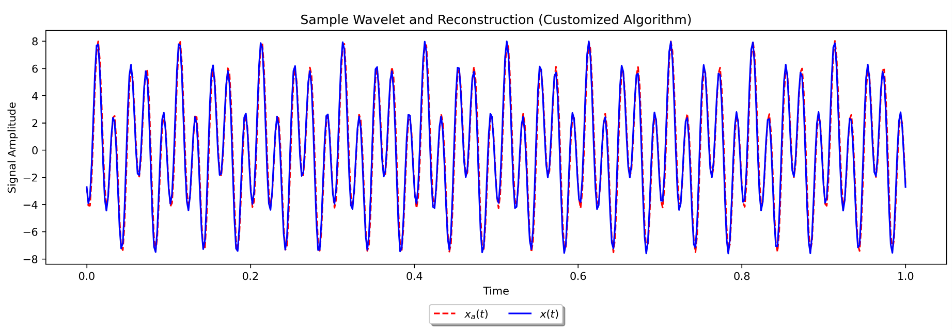
\includegraphics[width=0.8\textwidth]{Python_Wavelet_Transform_Plot_Combined.png} 
\caption{Sample Wavelet Plots (Main and Reconstructed Signals)} \label{fig:my_label}
\end{figure}


%\begin{table}[h]
%\centering
%\begin{tabularx}{0.8\textwidth} { 
 % | >{\raggedright\arraybackslash}X 
  %| >{\centering\arraybackslash}X 
  %| >{\raggedleft\arraybackslash}X | }
 %\hline
 %Method & Correction Factor & Flexibility \\
 %\hline
 %Customized Algorithm  & 1.0130  & High  \\
%\hline
%PyWavelet Package  & 1.0155  & Limited  \\
%\hline
%Scipy.signal Package  & ---  & No Algorithm  \\
%\hline
%\end{tabularx}
%\caption{Comparison of correction factor and flexibility between different methods (Figure 5).}
%\label{table:comparison}
%\end{table}

\begin{table}[h]
\centering
\begin{tabularx}{0.8\textwidth} { 
  | >{\raggedright\arraybackslash}X 
  | >{\centering\arraybackslash}X 
  | >{\raggedleft\arraybackslash}X | }
 \hline
 Method & Correction Factor & Flexibility \\
 \hline
 Customized Algorithm  & 1.0130  & High  \\
\hline
\end{tabularx}
\caption{Outline of properties for Customized algorithm (Figure 7).}
\label{table:comparison}
\end{table}

From the plots and table, the customized algorithm has the lowest correction factor and a high flexibility in terms of varying the parameters for accurate results. This factor represents how much the wavelet transform has modified the original signal in terms of relative magnitude. Specifically, a factor greater than 1 means that the modified signal has larger amplitude than the original signal, while a factor less than 1 means that the modified signal has smaller amplitude than the original signal. The next section discusses the main results of using our customized codes on real wavelet data from the recent Cassini missions (2004 to 2017).  

%......................................................................................
\subsection{Implementation Routine}
\subsubsection{Data acquisition}
To analyze the amplitude of spiral density waves in Saturn's C ring, we first obtained VIMS(Visual and Infrared Mapping Spectrometer) data on the C-ring structure, using Fourier analysis to break down the ring structure in terms of its individual frequency (wavelength) components. Specifically, we used data from the Cassini spacecraft, with epoch of 1o years, to obtain measurements of the density waves in the rings. The data consists of images of the rings taken by the spacecraft.
\subsubsection{Image processing}
To apply Fourier transforms to the spiral density waves in Saturn's rings, we will first need to convert the set of images of the visual infrared and mapping spectrograph occultations for the ring structure, into a set of brightness values with higher values corresponding to regions of higher particle density, and vice-versa. The processed images contain information about the density waves, such as the location and shape of the waves in the images, as well as their amplitudes.
\subsubsection{Fourier transform}
We will first use the Continuous Wavelet Transform (CWT) algorithm to transform the time series of the amplitude measurements into the frequency domain. This will allow us to also perform phase correction of the distorted signals, owing to blockage or distortion by the planetary body.
\subsubsection{Phase-Correction Algorithm In Fourier Space}
In general, phase-correction is commonly used in signal processing to correct for phase distortions or misalignments that may have occurred during data acquisition or processing. In the context of planetary science or planetary seismology, phase correction may be used to correct for phase shifts or time delays in seismic signals caused by the propagation of seismic waves through a planetary body with a complex internal structure, like Saturn. For example, in the case of an occultation geometry, where a spacecraft passes behind a planet or moon and its signal is blocked or distorted by the planetary body, the seismic signals received by the spacecraft may be affected by the planet's internal structure, which can introduce phase shifts or time delays. By applying phase correction to the wavelet transform of the seismic signal, it may be possible to remove or mitigate some of these phase shifts or time delays, allowing for more accurate analysis and interpretation of the seismic data.
\subsubsection{Signal Reconstruction}
Here, we average the resulting signals present in the whole wave occultation, after the phase-corrected has been performed. We will utilize our customized algorithm in Python computing language to recover our signals.
%\subsection{Analysis}
%We will analyse the results of the reconstructed Fourier transform to gain insights into the underlying physics of the system. This will involve comparing the results from different locations in the ring system and identifying any patterns or correlations with Saturn's interior dynamics.

\subsection{Main Signal Versus Reconstructed Signal}
Following the required implementations for the wavelet algorithms in Python, and using the Morlet wavelet as the required mother wavelet, the following plots show the comparisms for a particular case using a sample Satellite resonance spiral density wave, \textbf{Atlas 2:1}, as a case-study. 


\textbf{A. Average Wavelet Power:}
The average wavelet power is a measure of the energy or power of a signal at different scales and positions in both time and frequency domains. In this context, it is calculated by taking the square root of the sum of the squares of both components of our data arrays along a specified axis. This could be a representation of the overall power of the sample wavelet signal. The image plot visualizes the distribution of wavelet power across spatial wavelengths and radii. The x-axis typically represents spatial wavelengths (1/km), and the y-axis represents radii (typically in 1000 km units).

\textbf{B. Power of Average Phase-Corrected Wavelet:}
This variable represents the power of the average phase-corrected wavelet. Phase-corrected wavelets are often used to enhance specific features or remove noise in a signal, as explained previously. This represents the power after applying phase correction. The image plot displays the distribution of power for the phase-corrected wavelet, similar to the first plot.

\textbf{C. Power Ratio:}
This variable represents the power ratio, which is calculated by dividing Power of Average Phase-Corrected Wavelet by Average Wavelet Power. It indicates how the power of the phase-corrected wavelet compares to the overall wavelet power. The image plot provides a visual representation of this power ratio, showing areas where the phase correction enhances or reduces the power relative to the average wavelet power.

These plots help visualize and analyze the distribution of power and the impact of phase correction in the context of wavelet analysis. They can be valuable for identifying patterns or features in the data and understanding the effectiveness of phase correction techniques in signal processing (more to come below).

\vspace{0.5}

\textbf{Note:}
The \textbf{'plt.imshow'} function is used to create these image plots. The \textbf{'vmin'} and \textbf{'vmax'} parameters control the color scale, and the \textbf{'extent'} parameter specifies the range of values for the x and y axes. The \textbf{'plt.xlabel'} and \textbf{'plt.ylabel'} functions set labels for the x and y axes of each plot.

\begin{figure}[h]
\centering 
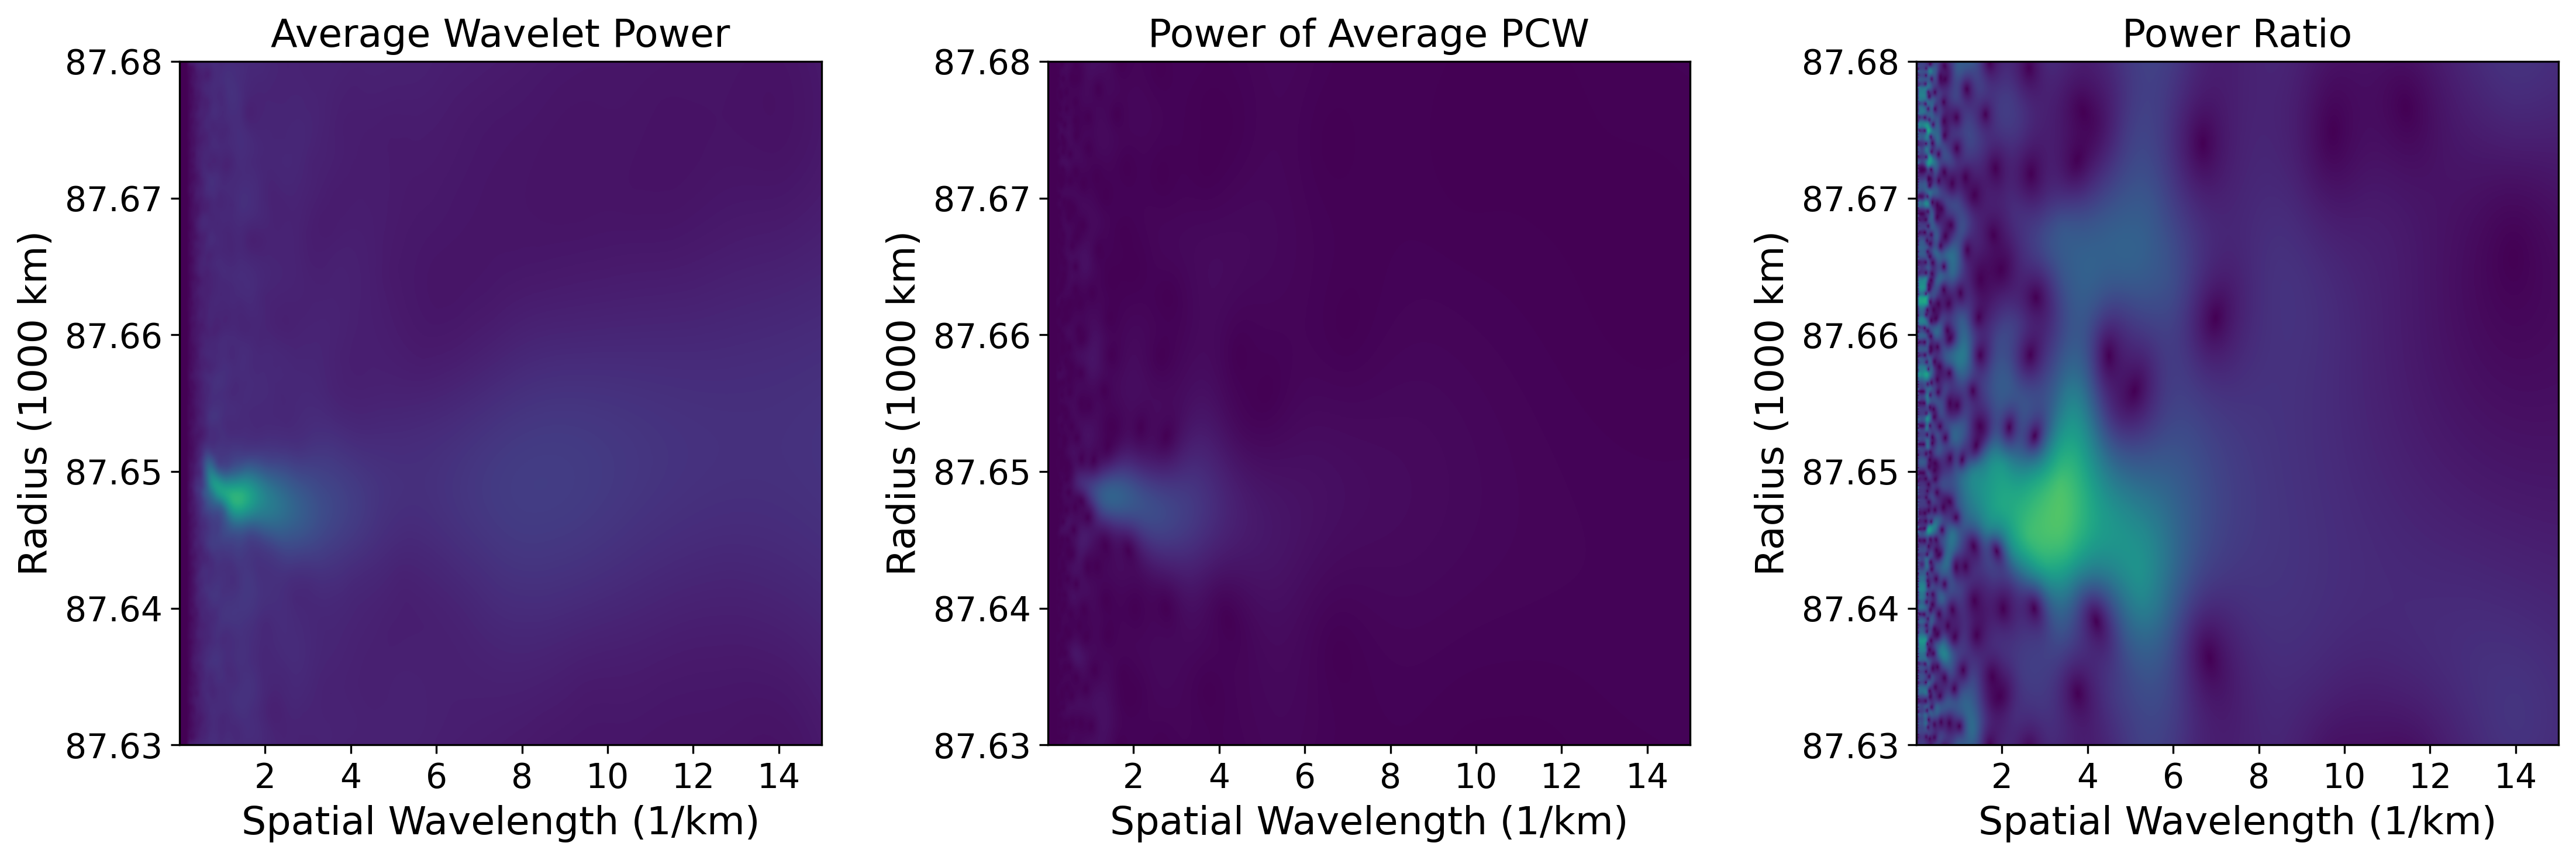
\includegraphics[width=1.0\textwidth]{power_ratio_plotw87.png} 
\caption{Plots for the Power Spectrum of the Satellite resonance wavelet signal, \textbf{Atlas 2:1}, reveal that it falls within the radial range of 87.64 - 87.65 (in units of 1000 kilometers) and exhibits a spatial wavelength between approximately 1 and 9 (per kilometer).} \label{fig:my_label}
\end{figure}


A final comparison is presented in Figure 9, showcasing reconstructed occultation profiles for this specific wavelet. The top plot (orange legend) represents the average background density variations associated with the signal. The initial reconstructed average wavelet (blue legend) is a cumulative representation of the occultation profiles contained within the wavelet data. The second reconstructed wavelet plot (green legend) is the first reconstructed average wavelet, which has been normalized to the background surface density in the region of Saturn's C-ring. It is evident that the wavelet reconstruction techniques perform exceptionally well in this particular case.

\begin{figure}
\centering 
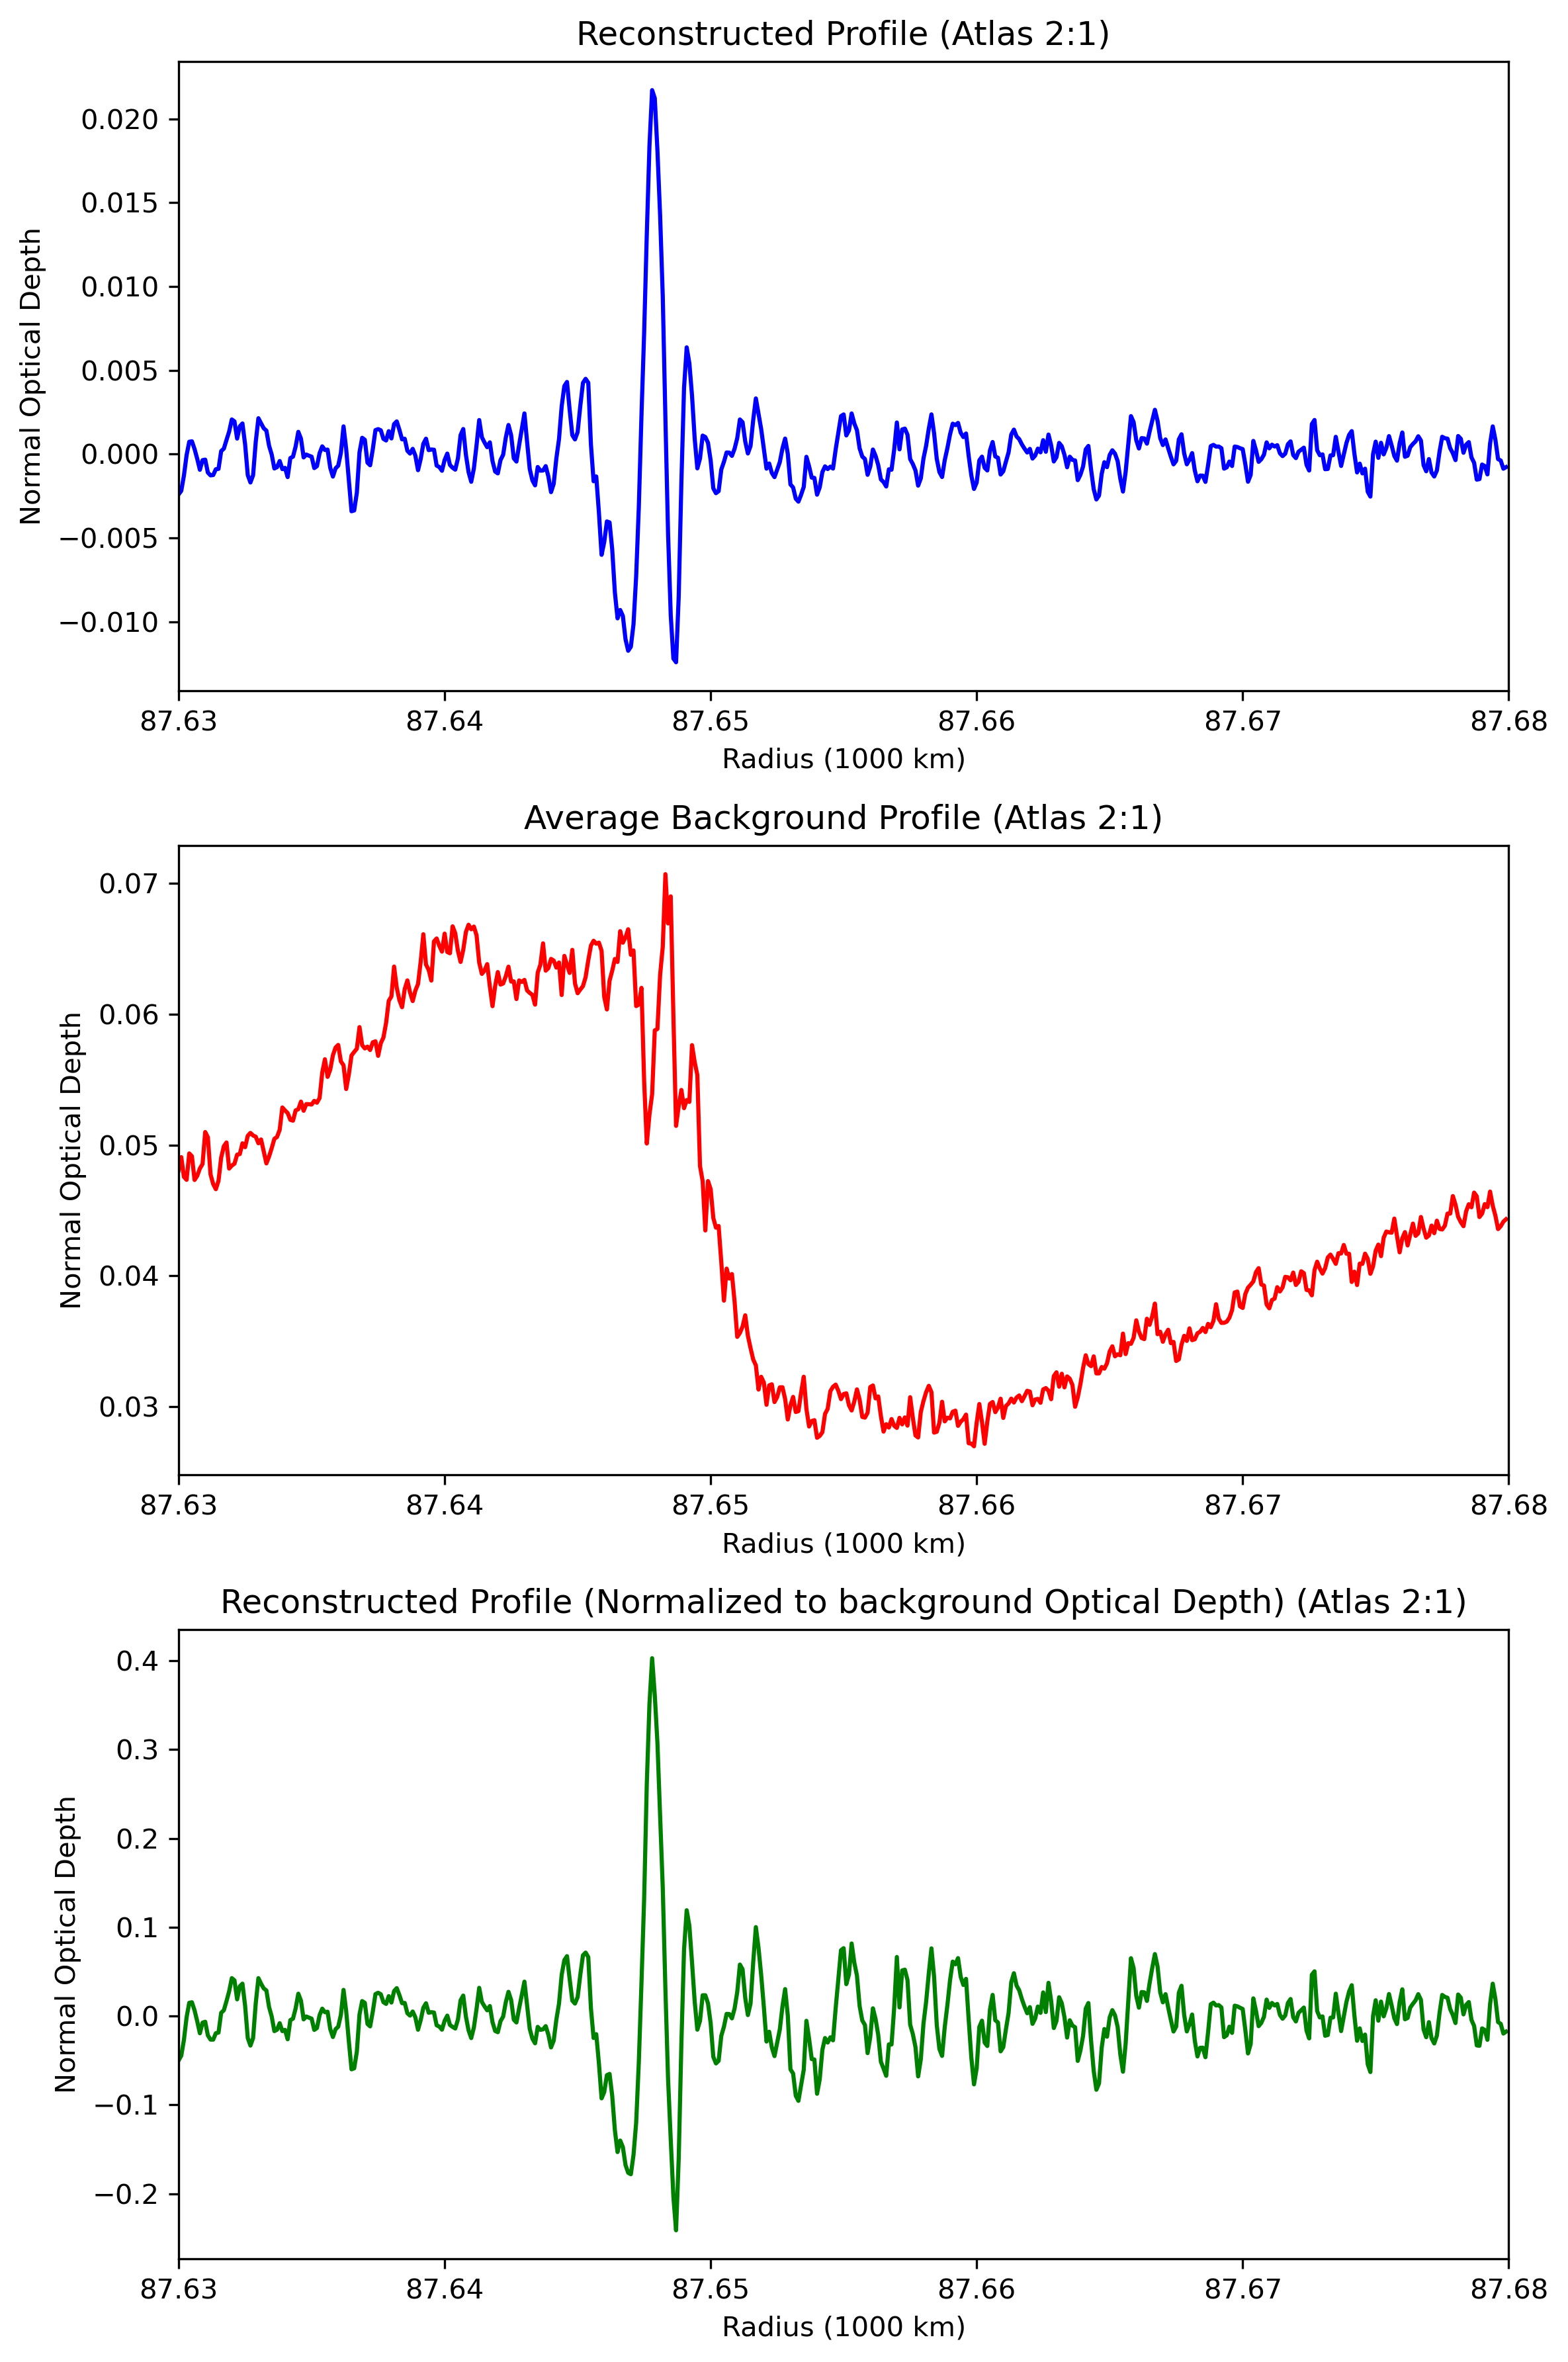
\includegraphics[width=0.85\textwidth]{combinedprofiles_atlas21.png}
\caption{A combined profiles for wavelet occultations for the Atlas 2:1 Satellite resonance.} \label{fig:my_label}
\end{figure}


%...............................................................................

\textbf{Final Note:}
The phase-correction algorithm applies phase shifts to the wavelet transform and then computes the average phase-corrected wavelets for each pattern speed. The captions describe two wave profile plots. In the first plot, the Normal Optical Depth is shown with a vertical offset, without phase correction. This plot highlights noisy wave profiles that are not properly aligned with expected results. In the second plot, the Normal Optical Depth is again displayed with a vertical offset, but this time with phase correction. Here, the wave profiles are less noisy and exhibit better alignment, as expected.

%The explained algorithm has led to significant findings regarding the behavior of waves in Saturn's rings. In particular, the wave analysed has proven to be strongly impacted by the planet's internal structure, including its rotation rate and density distribution, and not by any of Saturn's moons \cite{FRENCH2019599}\cite{Hedman_2018}. The study also discovered new information about the properties of these waves, such as the slightly changing positions of their amplitudes and some dips located along the regions of the detected waves, as evidenced in the plots of their optical depth profiles versus the radial distance \cite{BORDERIES1986522}. 

%\begin{figure}[h]
%\centering
%\begin{subfigure}[b]{1.1\textwidth}
 %  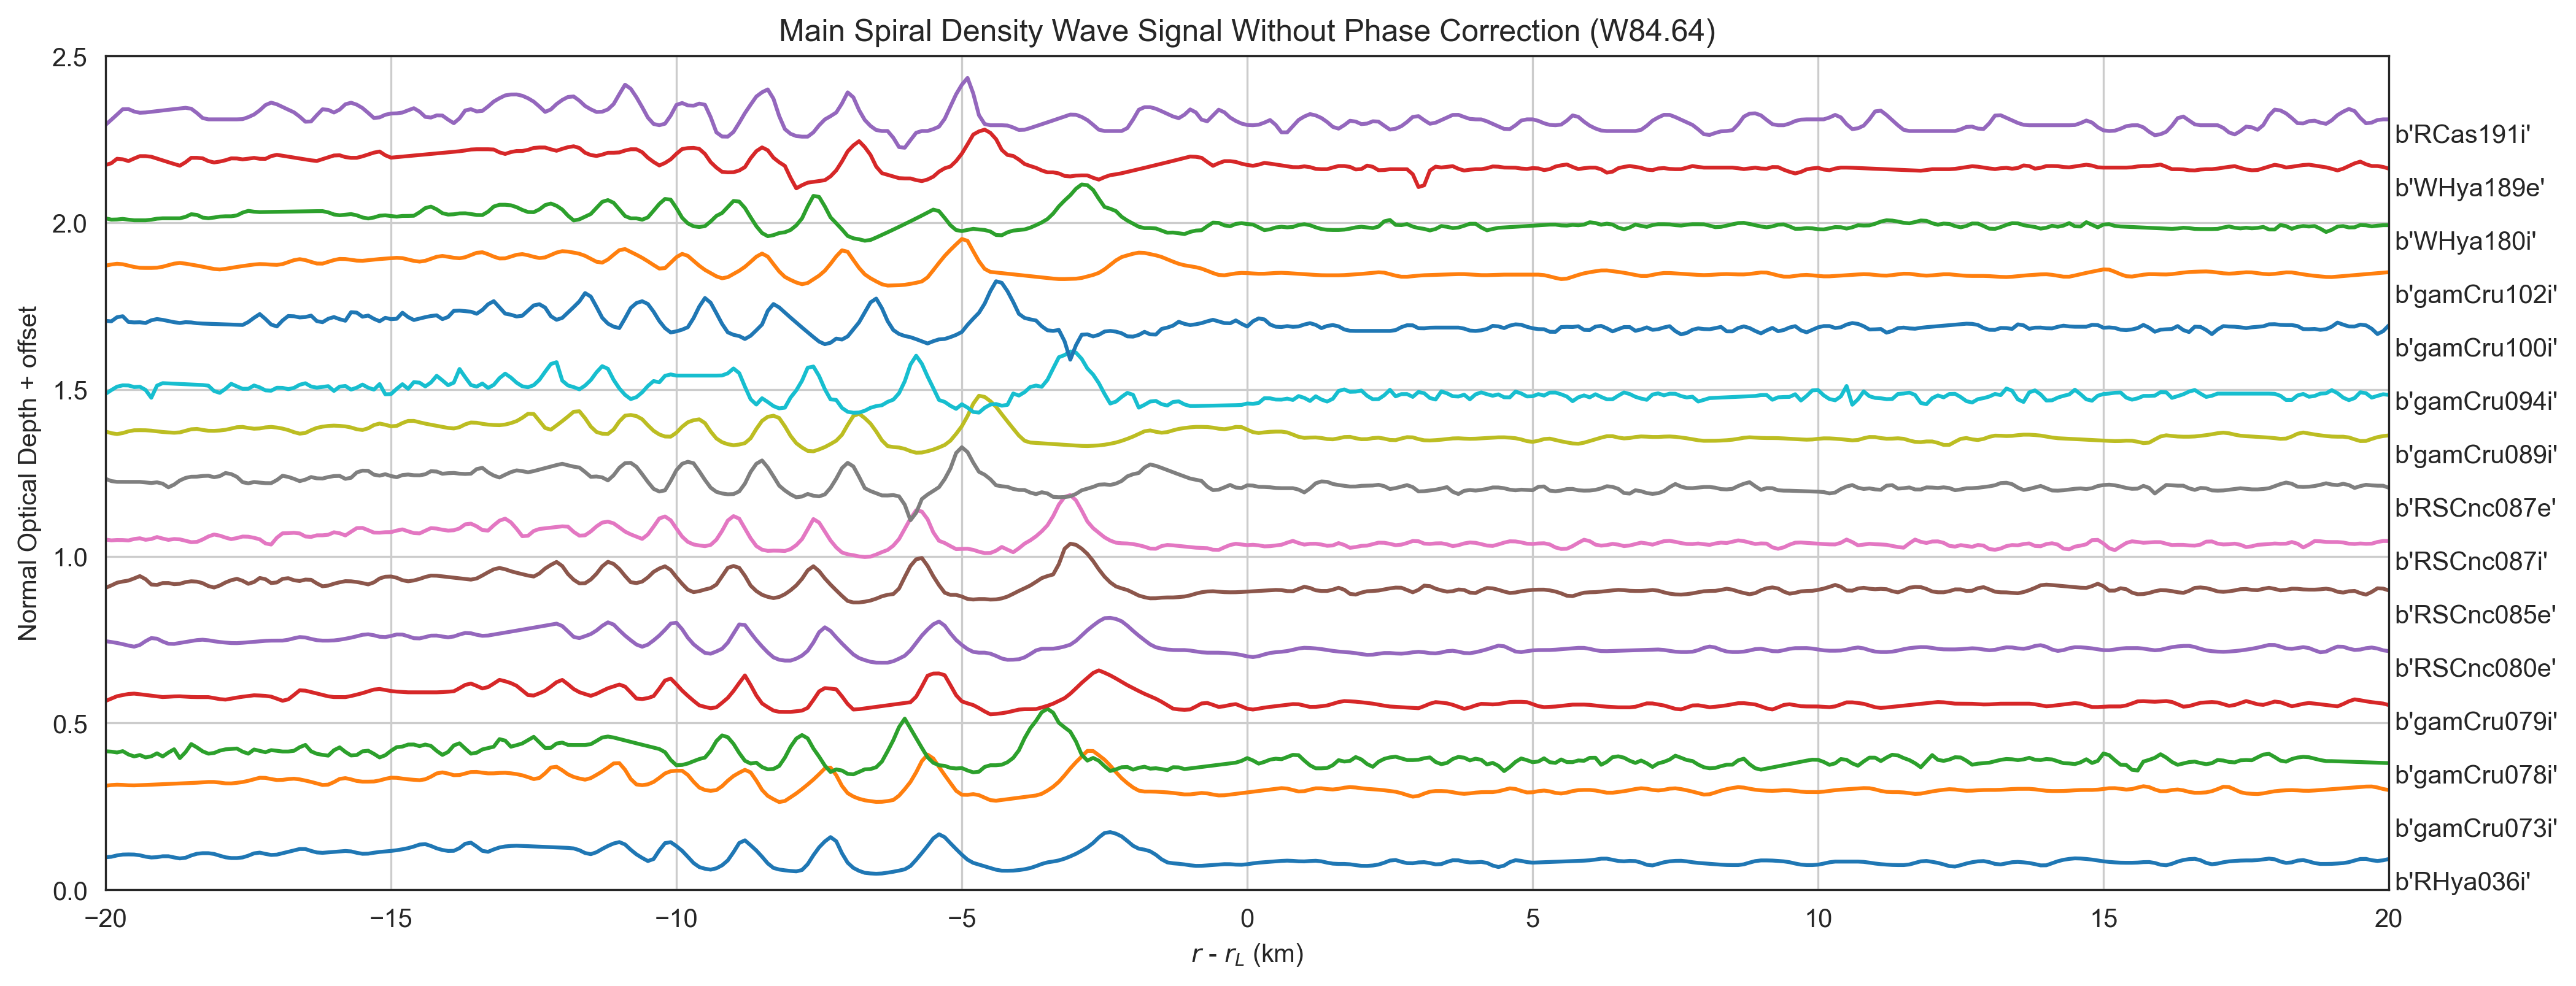
\includegraphics[width=0.9\linewidth]{Main_Main.png}
 %  \caption{}
  % \label{fig:Ng1} 
%\end{subfigure}
%\begin{subfigure}[b]{1.1\textwidth}
 %  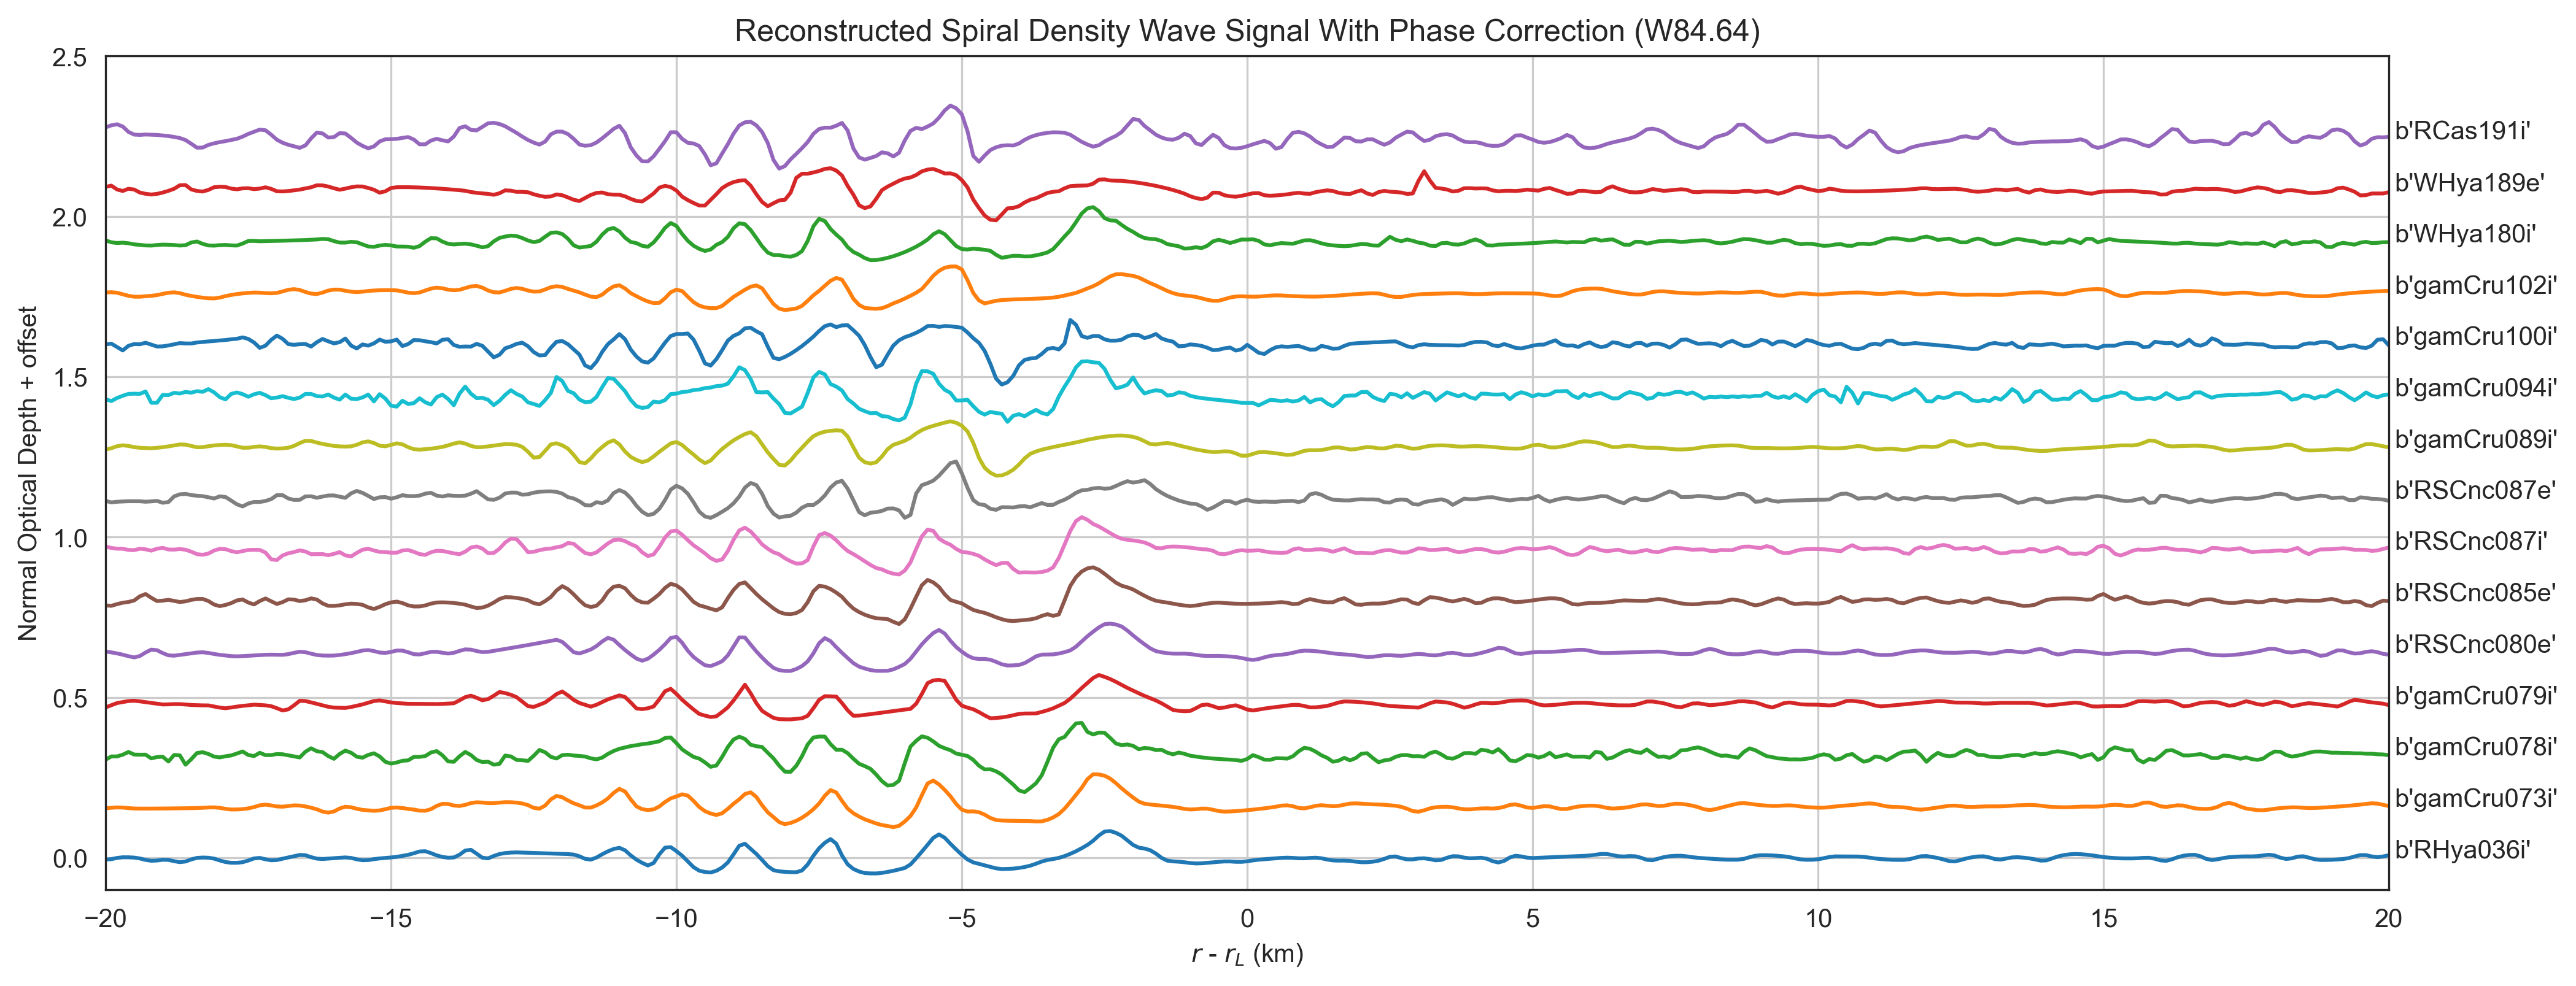
\includegraphics[width=0.9\linewidth]{Reconstructed_Main.png}
  % \caption{}
  % \label{fig:Ng2}
%\end{subfigure}
%\caption[Caption for Two Wave Profile Plots]{(a) Plot of the Normal Optical Depth (with vertical offset) for the wave profile (without phase correction). In this plot, the wave profiles exhibit noise and lack proper alignment. (b) Plot of the Normal Optical Depth (with vertical offset) for the wave profile (with phase correction). Here, the profiles appear less noisy and are mostly well-aligned.}
%\end{figure}


\begin{figure}[h]
    \centering
    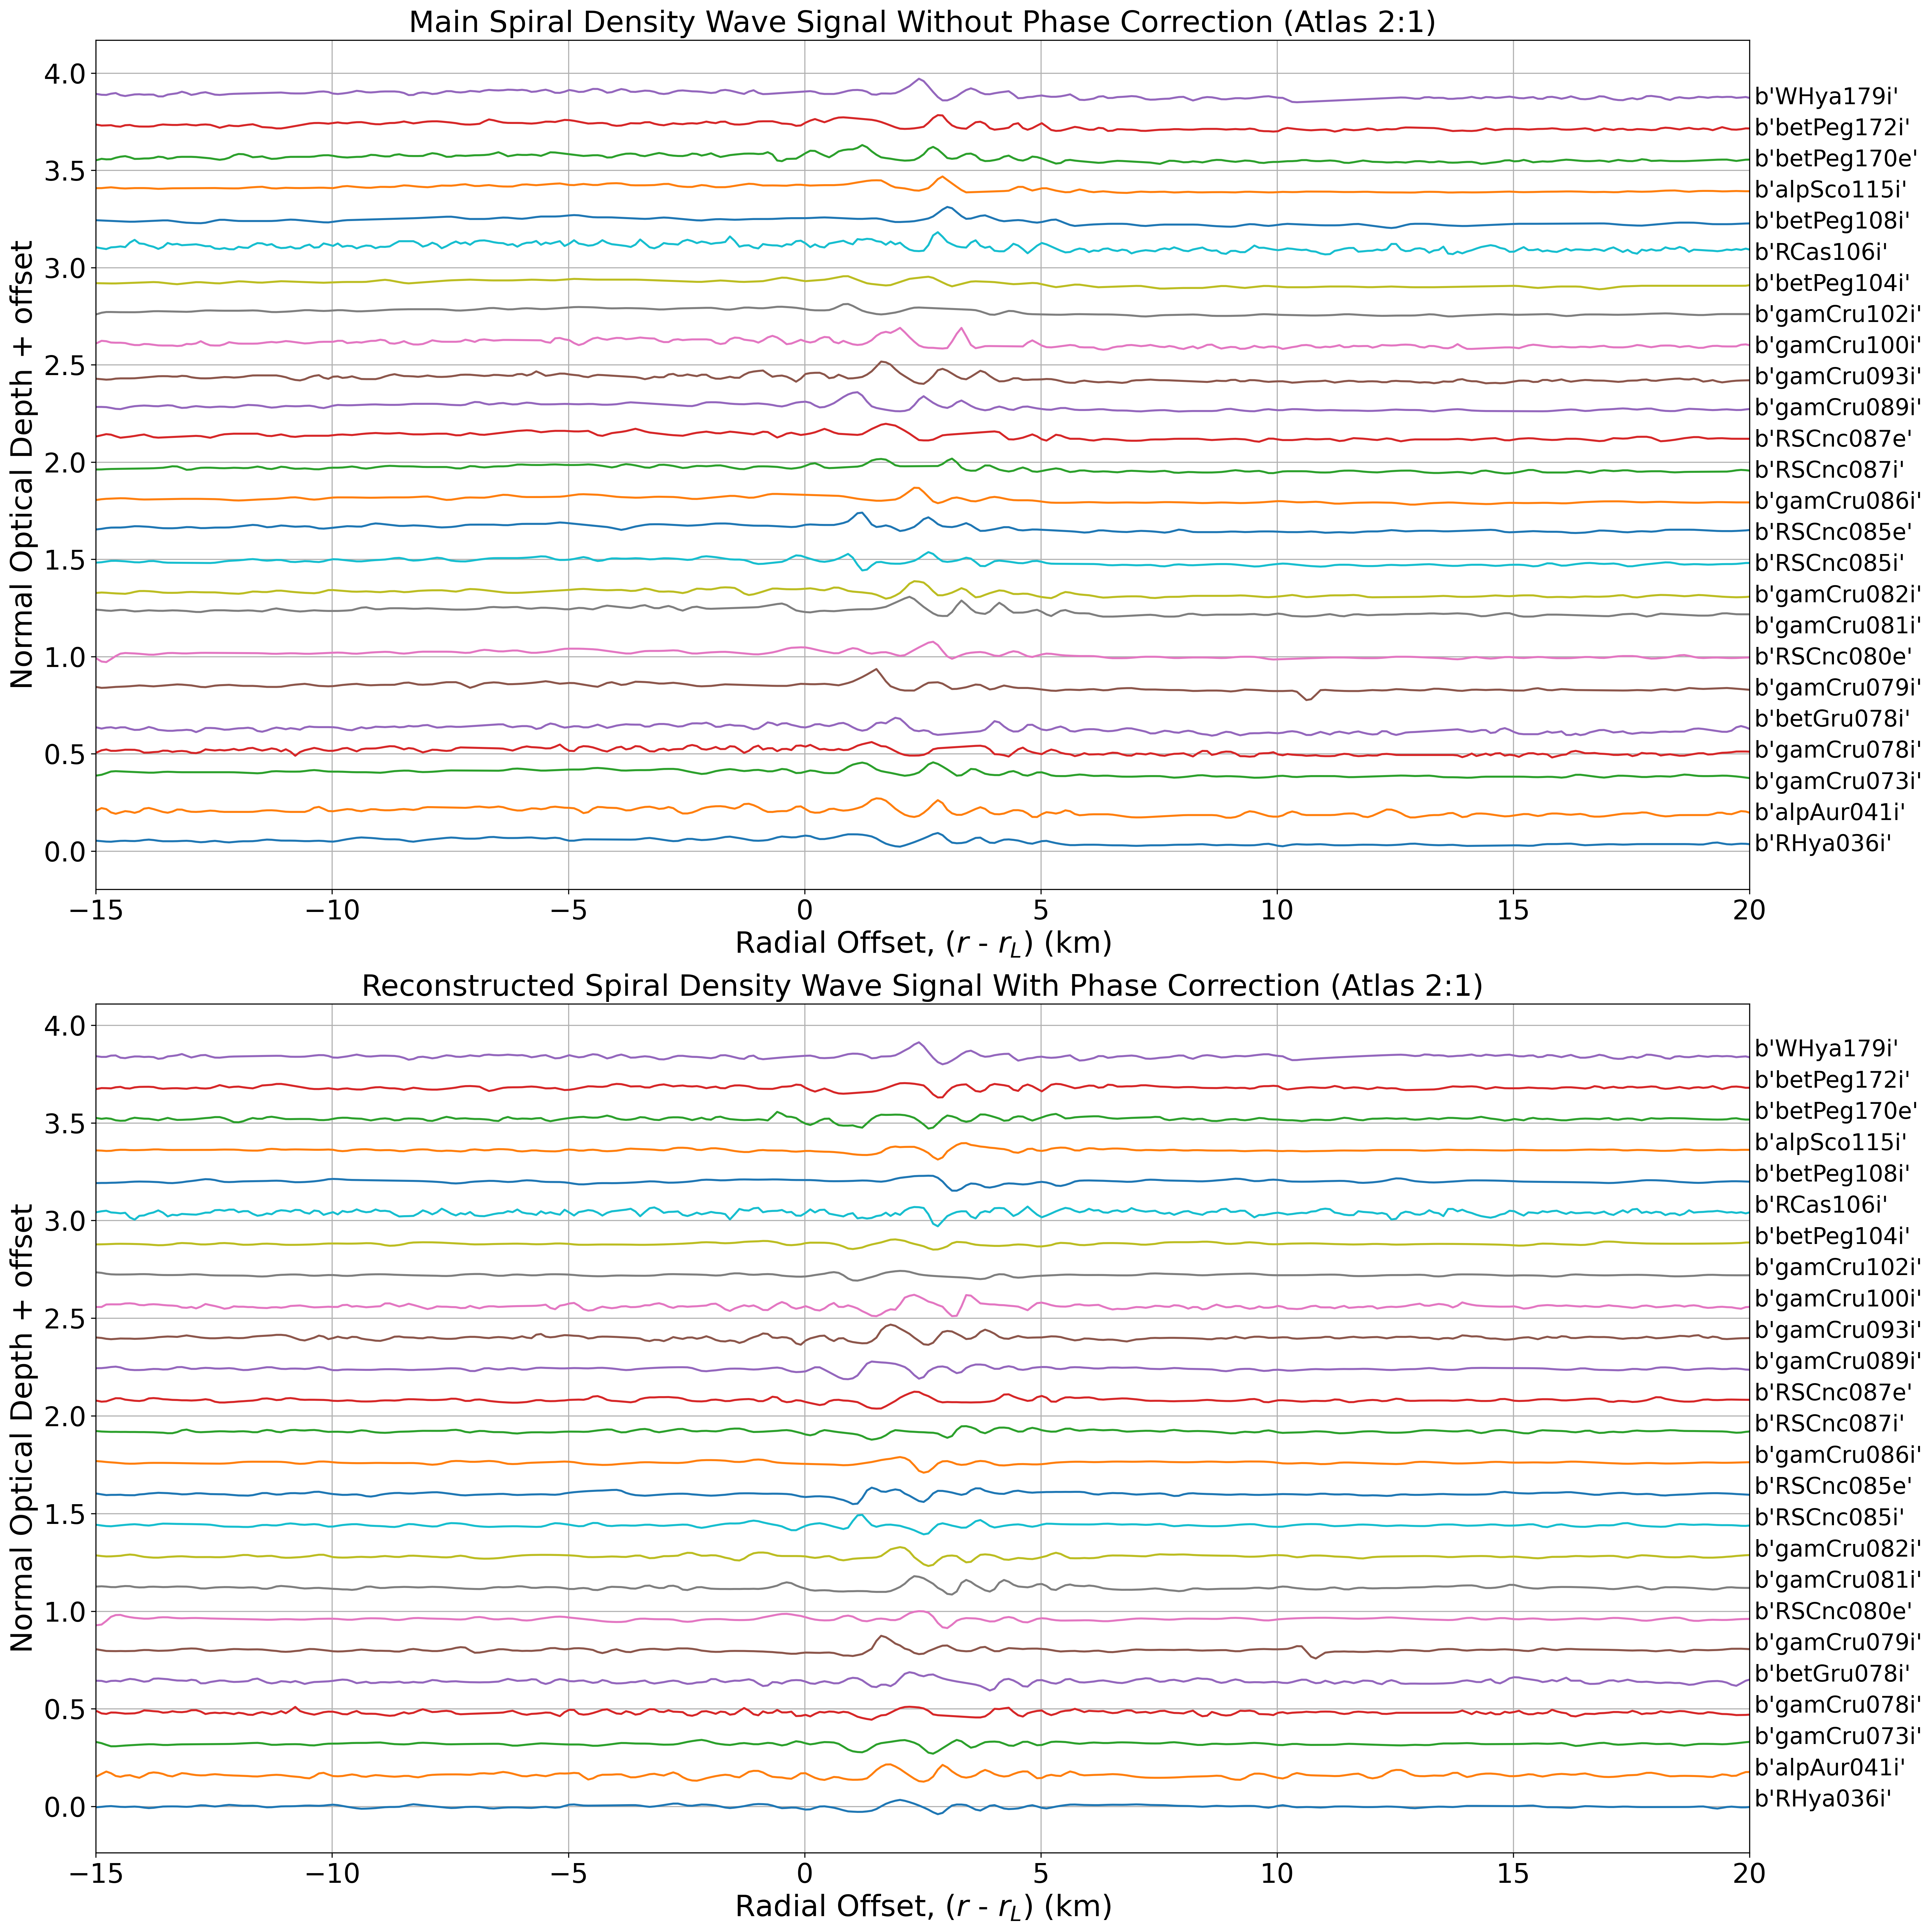
\includegraphics[width=1\linewidth]{main_and_reconstructed_profiles_atlas21_satellite_waves.png}
    \caption{[Upper Panel]: Plot of the Normal Optical Depth (with vertical offset) for the wave profile occultations (without phase correction). In this plot, the wave profiles exhibit noise and lack proper alignment in phase. [Lower Panel]: Plot of the Normal Optical Depth (with vertical offset) for the wave profile occultations (with phase correction). Here, the profiles appear less noisy and are mostly well-aligned in phase.}
    \label{fig:enter-label}
\end{figure}


\subsection{Wave-Fitting Routine}
In the process of gleaning the required information from the reconstructed signals, some pertinent parameters come to mind. 

Firstly, the surface mass density, $\sigma_{0}$, which represents the mass distribution across the section of the ring, around the region of the detected wave. It is a measure of the density of matter present in the wave. The wave-fitting process can be best achieved by determining the value of $\sigma_{0}$ that best fits the observed data. Secondly, viscosity, $\nu$, is associated with the region of the ring where the spiral density wave is located. It measures the resistance to the flow of matter within that region of the ring. Thirdly, the normal-mode amplitude coefficient, $C^{'}_{lmn}$, simply represents the spherical harmonic coefficient for Saturn's gravitational field, which could be interpreted as the amplitude of the planetary oscillation responsible for exciting spiral density waves across Saturn's (C)-ring(s). Thus, when considering the case where $n=0$, the amplitude coefficient simplifies to $C^{'}_{lmn}$, which also means the modes are fundamental in nature (as described above). In subsequent sections below, we present our steps for the wave-fitting routine.

\subsubsection{Surface Mass Density, $\sigma_{0}$}
Recall equation (6), $\xi = \left[\frac{3|m-1|\Omega_{L}^{2}r_{L}}{4\pi G \sigma_{0}}\right]^{\frac{1}{2}}\left(\frac{r-r_{L}}{r_{L}}\right)$. Let the coefficients of $(r-r_{L})$ be $\frac{1}{x_{f}}$. This implies:
\begin{equation}
 \frac{1}{x_{f}} = \left[\frac{3|m-1|\Omega_{L}^{2}r_{L}}{4\pi G \sigma_{0}}\right]^{\frac{1}{2}}\left(\frac{1}{r_{L}}\right),
\end{equation}
where $\Omega_{L}^{2} = \frac{G M_{P}}{r_{L}^{3}}$. When we substitute for $\Omega_{L}$, square both sides of the equation and perform further simplification, we could express $\sigma_{0}$ in terms of other parameters as:
\begin{equation}
 \sigma_{0} = \frac{3 |m-1| M_{P}x_{f}^{2}}{4\pi r_{L}^{4}}
\end{equation}

Here, $m$ is the azimuthal order of the wave signal. $x_{f}$ is the winding parameter from the Python Wave-fitting routine, measured in $Km$.  $r_{L}$ is the resonant radius of the wave-signal.  $M_{P}$ is the mass of Saturn ($5.6846 \times 10^{26}$ Kg). \textbf{Note:} The S.I. Unit of $\sigma_{0}$ corresponds with the standard measurement in $Kgm^{-2}$.


\subsubsection{Viscosity, $\nu$}
Assuming the damping phenomenon is insufficient to allow several wavecycles, we can estimate the ring section's kinematic viscosity, $\nu$, as in the case \cite{GOLDREICH1978240}\cite{1984prin.conf..513S}\cite{Tiscareno_2007}:
\begin{equation}
    \nu = \frac{9}{7\Omega_{L}\xi_{D}^{3}}\left(\frac{r_{L}}{\mathcal{D}_{L}}\right)^{1/2}(2\pi G \sigma_{0})^{3/2}
\end{equation}
 
 Where $\mathcal{D}_{L}$ = $3|m-1|\Omega_{L}^{2} + J_{2}(\frac{r_{s}}{r_{L}})^{2}[\frac{21}{2}-\frac{9}{2}|m-1|]\Omega_{L}^{2}$. The second term is only applicable as a correction factor for cases when $m \neq 1$.

Making substitutions for $\Omega_{L}$ and simplifying this equation, the viscosity becomes: 
\begin{equation}
    \nu = \frac{9}{7 x_{D}^{3}}(\frac{Gr_{L}^{7}}{M_{P}^{2}d_{L}})^{\frac{1}{2}}(2\pi\sigma_{0})^{\frac{3}{2}}
\end{equation}
 Where $d_{L}$ = $3|m-1| + J_{2}(\frac{r_{s}}{r_{L}})^{2}[\frac{21}{2}-\frac{9}{2}|m-1|]$. $x_{D}$ is the same as $\xi_{D}$, the dimensionless damping Parameter. The new term is required for the wave-fitting routine, as we shall see in subsequent procedures. $G = 6.674 \times 10^{-11}m^{3} Kg^{-1} s^{-2}$. $r_{s} = 60330$Km (Equatorial radius for Saturn). $J_{2} = 0.01629$ (For Saturn). \textbf{Note:} The S.I. Unit of $\nu$ corresponds with measurements in $m^{2}s^{-1}$.


\subsubsection{Saturn's Normal-mode Amplitude Calculations, $C_{lm0}^{'}$}
From \cite{Marley1993PlanetaryAM} and \cite{Zharkov1985ThePO}, we express the total gravitational potential of a planet as: \begin{equation}
    \Phi = \Phi_{0} + \Phi{'}
\end{equation}
Here, $\Phi_{0}$ = Unperturbed gravitational potential, given as: 
\begin{equation}
\Phi_{0} = \frac{GM}{r}\left\{1 - \sum_{l=1}^{\infty}\left(\frac{a}{r}\right)^{l}J_{l}P_{l}(\cos \theta) + \sum_{l=1}^{\infty}\sum_{m=1}^{l}\left(\frac{a}{r}\right)^{l}P_{l}^{m}(\cos \theta)[C_{lm}(\cos m\phi) + S_{lm}(\sin m\phi)]\right\}
\end{equation}

From \cite{Marley1993PlanetaryAM}, Saturn is a fluid planet in hydrostatic equilibrium, and hence there should be no permanent non-axisymmetric terms in the potential. This implies that $C_{lm}$ and $S_{lm}$ are presumed zero for Saturn.

By reason of the above-mentioned statement, we use $\Phi{'}$ = $\Phi{'}(t)$, time variable gravitational potential ( caused by the time variable density perturbations within Saturn). 

From \cite{Marley1993PlanetaryAM} \cite{Zharkov1985ThePO}, we have:
\begin{equation}
\Phi{'}(t) = \frac{GM}{r}\sum_{n=0}^{\infty}\left\{ - \sum_{l=2}^{\infty}\left(\frac{a}{r}\right)^{l}J_{ln}^{'}P_{l}(\cos \theta) + \sum_{l=2}^{\infty}\sum_{m=-l}^{l}\left(\frac{a}{r}\right)^{l}P_{l}^{m}(\cos \theta)[C_{lmn}^{'}(\cos m\phi) + S_{lmn}^{'}(\sin m\phi)]\right\}
\end{equation}
Note: $l$ = Angular degrees of the wave signals. $a$ = Equatorial radius of Saturn. $n$ = The mode of a particular wave signal (f-mode, $n$ = 0). 

Using the choice of phase, $\phi$ = 0 (is the azimuthal angle \cite{A’Hearn_2022}), $\cos m\phi$ = 1, and $\sin m\phi$ = 0, the equation becomes:
\begin{equation}
\Phi{'}(t) = \frac{GM}{r}\sum_{n=0}^{\infty}\left\{ - \sum_{l=2}^{\infty}\left(\frac{a}{r}\right)^{l}J_{ln}^{'}P_{l}(\cos \theta) + \sum_{l=2}^{\infty}\sum_{m=-l}^{l}\left(\frac{a}{r}\right)^{l}P_{l}^{m}(\cos \theta)C_{lmn}^{'}\right\}
\end{equation}

Since the wave signals have $m \neq 0$, $J_{ln}^{'}$ is negligible ($J_{ln}^{'}\approx 0$). The new expression becomes: 
\begin{equation}
\Phi{'}(t) = \frac{GM}{r}\sum_{n=0}^{\infty}\left\{\sum_{l=2}^{\infty}\sum_{m=-l}^{l}\left(\frac{a}{r}\right)^{l}P_{l}^{m}(\cos \theta)C_{lmn}^{'}\right\}
\end{equation}

Recall, we are considering wave signals that are assumed to mostly be from fundamental modes ($n$=0): 
\begin{equation}
\Phi{'}(t) = \frac{GM}{r}\left\{\sum_{l=2}^{\infty}\sum_{m=-l}^{l}\left(\frac{a}{r}\right)^{l}P_{l}^{m}(\cos \theta)C_{lm0}^{'}\right\}
\end{equation}


For understanding the angles, $\theta$ (the colatitude), we are evaluating the potential in the rings, which are at the planet’s equator plane, and taken to be at $90^{o}$ to the (imaginary) vertical axis passing through the center of the planet, Saturn [M. Hedman, personal discussion (June, 2022), additional information from \cite{Mankovich_2019}]. We take $\mu = \cos\theta = 0$, and the new equation becomes: 

\begin{equation}
\Phi{'}(t) = \frac{GM}{r}\left\{\sum_{l=2}^{\infty}\sum_{m=-l}^{l}\left(\frac{a}{r}\right)^{l}P_{l}^{m}(\mu)C_{lm0}^{'}\right\},
\end{equation}
where r is the radius \cite{A’Hearn_2022}.

Since we are considering fully normalized gravitational harmonic coefficients, we need to use the fully normalized Associated Legendre Polynomial functions. Considering the orthonormalized harmonics that are commonly used in
the seismology community \cite{Jekeli2007PotentialTA} \cite{2015JASS...32..247S} \cite{https://doi.org/10.1029/2018GC007529}, and using only $|m| \neq 0$ cases, this implies, $P_{l}^{|m|} (\mu) \rightarrow \bar{P}_{l}^{|m|} (\mu)$, where:

\begin{equation}
    \bar{P}_{l}^{|m|} (\mu) = \sqrt{\frac{{(2-\delta_{0,|m|})(2l+1)(l-|m|)!}}{{4\pi (l+|m|)!}}} P^{|m|}_{l} (\mu)
\end{equation}

Here, $\delta_{0,|m|}$ = Kronecker delta function ( $\delta_{0,|m|}$ = 0, $ \forall |m| \neq 0$). $\bar{P}_{l}^{|m|} (\mu)$ = Normalized Associated Legendre Function. $P^{|m|}_{l} (\mu)$ = Unnormalized Associated Legendre Polynomial function derived from the standard Legendre polynomials using the relations below:
\begin{equation}
    P^{|m|}_{l}(\mu) = (-1)^{|m|}(1-\mu^{2})^{\frac{|m|}{2}}\frac{d^{|m|}}{d\mu^{|m|}}P_{l}(\mu)
\end{equation}

and 
\begin{equation}
    P_{l}(\mu) = \frac{1}{2^{l}l!} \frac{d^{l}}{d\mu^{l}}(\mu^{2} - 1)^{l}
\end{equation}



\textbf{Note:} 

1. The $(-1)^{|m|}$ factor in equation (11) is known as the Condon–Shortley phase. It is mostly employed in the physics and seismology communities (e.g., Dahlen & Tromp, 1998; Varshalovich et al., 1988 \cite{https://doi.org/10.1029/2018GC007529}). 

\href{https://en.wikipedia.org/wiki/Associated_Legendre_polynomials}{https://en.wikipedia.org/wiki/Associated_Legendre_polynomials}

2. The unnormalized form of the aforesaid harmonics are widely used when only the lowest few degrees are of importance. But, in reality, we are considering signals with both low and high harmonic degrees, hence the need to use the normalized format of the equation(s) \cite{https://doi.org/10.1029/2018GC007529}. 

3. Please see the link attached for more details regarding the computations: 

\href{https://docs.scipy.org/doc/scipy/reference/generated/scipy.special.lpmv.html}{https://docs.scipy.org/doc/scipy/reference/generated/scipy.special.lpmv.html}.

\vspace{3}

\textbf{Rearragement of Equations:}

\vspace{3}

From equation (10) above, let $k_{\alpha} = \sqrt{\frac{{(2-\delta_{0,|m|})(2l+1)(l-|m|)!}}{{4\pi (l+|m|)!}}}$, so that we have: 

\begin{equation}
    \bar{P}_{l}^{|m|} (\mu) = k_{\alpha} P^{|m|}_{l} (\mu)
\end{equation}

We also need to rewrite equation (9) in its new (normalized) form: 

\begin{equation}
\bar{\Phi}{'}(t) = \frac{GM}{r}\left\{\sum_{l=2}^{\infty}\sum_{m=-l}^{l}\left(\frac{a}{r}\right)^{l}\bar{P}_{l}^{|m|}(\mu)\bar{C}_{l|m|0}^{'}\right\}
\end{equation}

Let $(\frac{a}{r})^{l} = a_{r}^{l}$, we have: 
\begin{equation}
\bar{\Phi}{'}(t) = \frac{GM}{r}\left\{\sum_{l=2}^{\infty}\sum_{m=-l}^{l}a_{r}^{l}\bar{P}_{l}^{|m|}(\mu)\bar{C}_{l|m|0}^{'}\right\}
\end{equation}

By change of subject formula:

\begin{equation}
\sum_{l=2}^{\infty}\sum_{m=-l}^{l}\bar{C}_{l|m|0}^{'} = \sum_{l=2}^{\infty}\sum_{m=-l}^{l}\frac{(\bar{\Phi}{'}(t))(r)}{(GM)(a_{r}^{l})(\bar{P}_{l}^{|m|}(\mu))}
\end{equation}

Further simplification gives us: 
\begin{equation}
\sum_{l=2}^{\infty}\sum_{m=-l}^{l}\bar{C}_{l|m|0}^{'} =\frac{r}{GM} \sum_{l=2}^{\infty}\sum_{m=-l}^{l}\frac{\bar{\Phi}{'}(t)}{(a_{r}^{l})(\bar{P}_{l}^{|m|}(\mu))}
\end{equation}

Note: 
We intentionally left $\bar{\Phi}{'}(t)$ at the numerator, and after the summation symbols, because this parameter is a function of $l$ and $m$, as we shall see in the next section. 

\vspace{3}

\paragraph{Link With Wave-Fit Amplitude:}

\vspace{3}

To succinctly link the wave-fit amplitude to the gravitational potential for the planetary normal-mode oscillation, we solve for a self-consistent solution for the perturbed gravitational potential of the disk \cite{1984prin.conf..513S}, $\Phi_{D}(r,\lambda,t) = \Phi_{D}(r)e^{i(\omega t - m \lambda)}$; where $\Phi_{D}(r)$ is of the form $A(r)exp[i\int k dr]$. The surface density perturbation is obtained from the derivative of the disk potential, using equation (34) in \cite{1984prin.conf..513S}:
\begin{equation}
    S(r) = - \frac{|k(r)|A(r)}{2\pi G},
\end{equation}
where $k(r)$ is the radial wavenumber. The final result for a density wave driven at an ILR or an OLR has a radial dependence given by:
\begin{equation}
    \Phi_{D}(r) = A_{L}H_{q}(\xi),
\end{equation}
where the complex function $H_{q}(\xi)$ is specified in equation (47) of \cite{1984prin.conf..513S} and plotted in figure 5 therein. A variant of it has been solved previously on here as well. Far from resonance, $H_{q}(\xi)$ oscillates about zero with a constant amplitude of $\pm1$. The amplitude factor, $A_{L}$, is determined by the amplitude of the driving term in the satellite potential $\Phi_{m}^{'}$ and the background surface mass density $\sigma_{0}$ through the the equation:
\begin{equation}
    A_{L} = \mp\sqrt{2\pi|\epsilon|}\Psi_{m}^{'},
\end{equation}
where the dimensionless parameter $\epsilon$ is defined as in \cite{1984prin.conf..513S} equation (45b) as:
\begin{equation}
    \epsilon = \frac{2\pi G \sigma_{0}}{r_{L}^{2}(dD/dr)_{L}} = \mp \frac{2\pi G \sigma_{0}}{3(m\pm1)n^{2}r_{L}},
\end{equation}

which is applicable near resonance, for $m \neq 1$. Using Kepler's third law and rewriting the mean motion $n$ in terms of Saturn's mass, we observe that $\epsilon \sim \mathcal{O} \left({m_{\text{ring}}}/{M_{\text{Saturn}}}\right) \simeq 10^{-8}$. Near a Lindblad resonance, the dispersion relation can be rewritten in terms of the small parameter $\epsilon$, as:

\begin{equation}
    |k(r)| \simeq \frac{r - r_{L}}{\epsilon r_{L}^{2}}.
\end{equation}

Since $k(r) \propto (r - r_{L})$ in the neighborhood of a Lindblad resonance, the surface density perturbation is predicted to grow linearly with distance from the resonance location. As $A_{L} \propto \sigma_{0}^{1/2}$ while $k(r) \propto \sigma_{0}^{-1}$, the absolute amplitude of the density wave driven at a Lindblad resonance is expected to scale as $\sigma_{0}^{-1/2}$, at a given distance from the resonance location. Here, the fractional amplitude of the wave $S(r)/\sigma_{0}$ should scale as $\sigma_{0}^{-3/2} (\cite{1984prin.conf..513S}, Nicholson's Memo.)$:
\begin{equation}
    \frac{S(r)}{\sigma_{0}} = - \sqrt{\frac{2\pi}{\epsilon^{3}}} \frac{(r - r_{L})}{3(m \pm 1) n^{2} r_{L}^{3}} \Psi_{m}^{'}.
\end{equation}

In practice, there are some notable effects regarding the aforesaid description for density waves and their evolution in the planetary rings:

\textbf{1. Nonlinear Behavior:} The wave amplitudes observed in planetary rings become nonlinear within the first few wavelengths from the resonance. Nonlinear behavior in waves means that the relationship between the wave's amplitude and its driving force is not proportional.

\textbf{2. Limit on Amplitude:} The nonlinearity in waves imposes a limit on their maximum amplitudes. This suggests that as the waves propagate, their amplitudes cannot keep growing without bounds.

\textbf{3. Dissipation within the Disk:} Eventually, the wave amplitudes damp due to dissipation within the disk. Dissipation refers to the process of energy loss in the system. In this context, it's occurring within the planetary ring's disk.

\textbf{4. Causes of Dissipation:} The dissipation is attributed largely to inelastic collisions within the disk. Inelastic collisions involve a loss of kinetic energy, and this process contributes to the damping of wave amplitudes. The amplitude decays as $exp[-(|r - r_{L})/r_{D}|)^{3}]$, where $r_{D}$ is a damping length set by the disk's viscosity (\cite{1984prin.conf..513S}, equations (62) and (63)). By employing a streamlined approach, we can sidestep the intricacies associated with estimating ring viscosity. Instead, we opt for an approximate determination of the density wave's maximum amplitude. This is achieved by computing the anticipated amplitude at a consistent number of radial wavelengths from the resonance point, aligning with a fixed value of the radial phase, say $\phi(r) = \phi_{0}$. This method allows for a more straightforward assessment of the density wave characteristics, offering a practical alternative to the complex task of directly estimating ring viscosity. Note that, 
\begin{equation}
    \phi(r) = \int_{r_{L}}^{r} k(r) dr,
\end{equation}
and substituting for $k(r)$ from equation (73), we have:
\begin{equation}
    \phi(r) = s \frac{(r - r_{L})^2}{2 \epsilon r_{L}^{2}},
\end{equation}
noting that $\epsilon$ is negative for an OLR. The corresponding distance from the boundary condition, $\phi(r) = \phi_{0}$, is given as:
\begin{equation}
    r_{0} - r_{L} = \mp \sqrt{2 s \epsilon \phi_{0}} r_{L},
\end{equation}
noting again that $s = \mathrm{sgn}(k)$. At this location, the radial wavenumber is given as: 
\begin{equation}
    |k_{0}(r)| = \sqrt{\frac{2s\phi_{0}}{\epsilon}}\left(\frac{1}{r_{L}}\right),
\end{equation}
causing it to scale as $\sigma_{0}^{-1/2}$. The expression for the wave amplitude at $r_{0}$ becomes:
\begin{equation}
    S(r_{0}) = \pm \frac{\Psi_{m}^{'}}{G r_{L}} \sqrt{\frac{s \phi_{0}}{\pi}} = \pm \frac{\Psi_{m}^{'}}{G r_{L} \sqrt{2\pi\epsilon}}\frac{(r_{0} - r_{L})}{r_{L}}.
\end{equation}

Recall that $\epsilon = \mp \frac{2\pi G \sigma_{0}}{3(m\pm1)n^{2}r_{L}}$ and $n^{2} = G M_{P}/r_{L}^{3}$. Substituting into the equation (79), we have the result as:
\begin{equation}
    S(r_{0}) = \pm \frac{\Psi_{m}^{'}}{G r_{L}} \sqrt{\frac{3(m\pm1)M_{P}}{4\pi^{2} \sigma_{0}r_{L}^{2}}}   \frac{(r_{0} - r_{L})}{r_{L}}.
\end{equation}

In its fractional form, with respect to the background surface mass density $\sigma_{0}$, the generalized form of the factor-ed amplitude becomes:
\begin{equation}
   \frac{S(r)}{\sigma_{0}} = \pm \frac{\Psi_{m}^{'}}{\sqrt{\pi}G\sigma_{0} r_{L}} \sqrt{\frac{3|m - 1|M_{P}}{4 \pi \sigma_{0}r_{L}^{2}}} \frac{(r - r_{L})}{r_{L}}.
\end{equation}

Ultimately, we can say that:
\begin{equation}
  A_{\sigma_{0}}(r) = \pm \frac{\Psi_{m}^{'}}{\sqrt{\pi}G\sigma_{0} r_{L}} \sqrt{\frac{3|m - 1|M_{P}}{4 \pi \sigma_{0}r_{L}^{2}}} \frac{(r - r_{L})}{r_{L}}e^{-(|(r - r_{L})/r_{D}|)^{3}},
\end{equation}
where $\xi = \sqrt{\frac{3|m - 1|M_{P}}{4 \pi \sigma_{0}r_{L}^{2}}}\frac{(r - r_{L})}{r_{L}}$ holds the same meaning as equation (10) from \cite{Nicholson1990AnAR}. Exploring density wave signals within the context of normalized background surface density and optical depth fluctuations is essential for a comprehensive understanding of its dynamics. In this intricate analysis, it becomes imperative to articulate the amplitude of the wave in terms of its fractional form. By doing so, we delve into a nuanced examination of the intricate interplay between density variations and optical depth, unraveling deeper insights into the underlying dynamics. This approach not only enhances the precision of our observations but also paves the way for a more thorough exploration of the intricate patterns and behaviors exhibited by these density waves.


From the Python Wave-Fitting routine, the wave profile is given as a variant of equation (30):
\begin{equation}
    y(x) = a(\frac{x-x_{r}}{x_{f}})e^{-\frac{(|x-x_{r}|)^{3}}{(x_{d}x_{f})^{3}}}\cos\left[\phi_{0} - \frac{3\pi}{4} - \frac{{(x-x_{r})^2}}{{x_{f}^{2}}}\right]\zeta(\frac{x-x_{r}}{x_{f}}), 
\end{equation}
where,  $\zeta(\frac{x-x_{r}}{x_{f}})$ is similar to  $\zeta(\xi)$, but it has been customized to account for waves with differing azimuthal orders, m.            

\begin{equation}
\zeta(\frac{x-x_{r}}{x_{f}}) = [1 + \mathrm{sgn}(m) \mathrm{sgn}(\frac{x-x_{r}}{x_{f}})],
\end{equation}
and $\mathrm{sgn}(m) \mathrm{sgn}(\frac{x-x_{r}}{x_{f}})]$ = \left\{ \begin{array}{rcl}
+1 & \forall & m, (\frac{x-x_{r}}{x_{f}}) >0;  m, (\frac{x-x_{r}}{x_{f}}) <0  \\ 0 & \forall & m =0; (\frac{x-x_{r}}{x_{f}}) = 0 \\ -1 & \forall & m<0, (\frac{x-x_{r}}{x_{f}}) >0; m>0, (\frac{x-x_{r}}{x_{f}}) <0 \\ 
\end{array}\right\}$

\vspace{5}

Let the direct amplitude of the Wave-fit routine be given as:
\begin{equation}
    a(x) = a(\frac{x-x_{r}}{x_{f}})e^{-\frac{(|x-x_{r}|)^{3}}{(x_{d}x_{f})^{3}}}[1 + \mathrm{sgn}(m) \mathrm{sgn}(\frac{x-x_{r}}{x_{f}})]
\end{equation}

The component, $\zeta(\frac{x-x_{r}}{x_{f}})$ is only relevant in the wave-fitting procedure. Since the wave signals are usually detected at particular resonance locations, for both the retrograde ($m<0$) and prograde ($m>0$) cases, this implies that $\zeta(\frac{x-x_{r}}{x_{f}}) \rightarrow 2, \forall  x \in (-\infty,+\infty)$ respectively.

Hence,
\begin{equation}
    a(x) = 2a(\frac{x-x_{r}}{x_{f}})e^{-\frac{(|x-x_{r}|)^{3}}{(x_{d}x_{f})^{3}}}
\end{equation}

Here, we treat both non-exponential terms for equations (82) and (86) on the basis that $a(x) = A_{\sigma_{0}}(r) \rightarrow r-r_{L} = x-x_{r}$:
\begin{equation}
    \frac{2a}{x_{f}} = \frac{\Psi^{'}_{m}}{\sqrt{\pi} G\sigma_{0}r_{L}^{2}}\sqrt{\frac{3|m-1|M_{P}}{4\pi\sigma_{0}r_{L}^{2}}}
\end{equation}
Assuming $a = a_{fit}$, the dimensionless amplitude derived from the wave-fitting routine, we can reshuffle the equation (87) to become:
\begin{equation}
   \Psi^{'}_{m} = \ 2a_{\text{fit}} \frac{\sqrt{4\pi^{2}\sigma_{0}^{3}G^{2}r_{L}^{6}}}{\sqrt{3|m-1|M_{P} x_{f}^{2}}}
\end{equation}

Recall, from \cite{Hedman_2022}\cite{Marley1993PlanetaryAM}, equation (19), we provide the link between the planetary perturbation potential and that from the density wave oscillations across the ring as:
\begin{equation}
    \Psi^{'}_{m} = r \frac{d \bar{\Phi}{'}(t)}{dr} \pm 2m\bar{\Phi}{'}(t).
\end{equation}

The given equation is a first-order linear partial differential equation. It involves a partial derivative with respect to $r$ and describes a relationship between the functional perturbation potentials, $\Phi^{'}_{m}$ and $\bar{\Phi}{'}(t)$ (for the density wave across the ring surface and the planet, respectively) and $r$. The presence of the partial derivative indicates that the equation involves more than one independent variable. Resolution of the differential equation results to the general solution, say $\bar{\Phi}{'}(t) = \Phi{'}_{lm0}$:
\begin{equation}
   \Psi^{'}_{m} = (2m +l+1)\Phi{'}_{lm0}.
\end{equation}

This is a standard planetary model of degree $l$ and azimuthal wavenumber, $m$. $\Phi{'}_{lm0}$ is the relevant component of the planet’s gravitational potential due to that normal-mode oscillation. 

For our case, we have: $\Phi{'}_{l|m|0} = \frac{\Psi^{'}_{m}}{(2|m| + l + 1)}$. Recall, equation (68): $\sum_{l=2}^{\infty}\sum_{m=-l}^{l}\bar{C}_{l|m|0}^{'} =\frac{r}{GM} \sum_{l=2}^{\infty}\sum_{m=-l}^{l}\frac{\bar{\Phi}{'}(t)}{(a_{r}^{l})(\bar{P}_{l}^{|m|}(\mu))}$. 

Let $\Phi{'}_{l|m|0} = \bar{\Phi}{'}(t)$. This is the component of the time varying gravitational potential required to estimate the normal-mode amplitudes for Saturn, considering the wave signals detected. 

The new equation (68) becomes: 
\begin{equation}
    \sum_{l=2}^{\infty}\sum_{m=-l}^{l}\bar{C}_{l|m|0}^{'} =\frac{r}{GM} \sum_{l=2}^{\infty}\sum_{m=-l}^{l}\frac{{\Phi}^{'}_{l|m|0}}{(a_{r}^{l})(\bar{P}_{l}^{|m|}(\mu))}
\end{equation}

\textbf{Normal-mode Amplitude (N.M.A)} = \sum_{l=2}^{\infty}\sum_{m=-l}^{l}\bar{C}_{l|m|0}^{'}


\paragraph{Alternative Expression for $\Psi^{'}_{m}$:}
%From \cite{Nicholson1990AnAR}, we recall that the amplitude factor, $A_{L}$, may be calculated in terms of the perturbing satellite’s mass, $\mathcal{M}_{s}$, the orbital distance, $a_{s}$, and the background surface mass density of the ring(s), $\sigma_{0}$, as:

In accordance with the insights from \cite{Nicholson1990AnAR}, it is pertinent to revisit the computation of the amplitude factor, denoted as $A_{L}$. This crucial parameter can be effectively determined by considering key variables, namely the mass of the perturbing satellite denoted as $\mathcal{M}_{s}$, the orbital distance represented by $a_{s}$, and the background surface mass density characterizing the respective ring(s), denoted as $\sigma_{0}$.

The amplitude factor, $A_{L}$, serves as a fundamental metric in understanding the dynamic interactions within the celestial environment. Its calculation involves a nuanced interplay of variables, reflecting the intricate relationship between the perturbing satellite's mass, the orbital distance it maintains, and the background density of the surrounding ring structures.

Expressed mathematically, the relationship governing the determination of $A_{L}$ can be articulated as a function involving $\mathcal{M}_{s}$, $a_{s}$, and $\sigma_{0}$: 
\begin{equation}
    A_{L} = \frac{\mathcal{M}_{s}}{2\sqrt{\pi}a_{s}r_{L}\sigma_{0}}\left[\alpha \frac{d b_{1/2}^{m}}{d \alpha} + 2mb_{1/2}^{m}\right],
\end{equation}
where $\alpha = a/a_{s}$, a dimensionless ratio that is dependent on the orbital distance and $b_{1/2}^{m}(\alpha)$ is a Laplace coefficient given as\cite{1961mcm..book.....B}\cite{murray_dermott_2000}\cite{1984prin.conf..513S}\cite{articleTisHar}:
\begin{equation}
    b_{1/2}^{m}(\alpha) = \frac{2}{\pi} \int_{0}^{\pi} \frac{\cos(m \theta)}{\sqrt{1 - 2 \alpha \cos(\theta) + \alpha^2}} \, d\theta.
\end{equation}
Let $\Upsilon (m, \alpha) = \left[\alpha \frac{d b_{1/2}^{m}}{d \alpha} + 2mb_{1/2}^{m}\right]$, we can rephrase equation (92) as:
\begin{equation}
    A_{L} = \frac{\mathcal{M}_{s}}{2\sqrt{\pi}a_{s}r_{L}\sigma_{0}}\Upsilon (m,\alpha).
\end{equation}

From equation(82), let $A_{L} = \frac{\Psi_{m}^{'}}{\sqrt{\pi}G\sigma_{0} r_{L}}$, and solving with respect to equation (94), we have:
\begin{equation}
  \Psi_{m}^{'} =  \frac{G \mathcal{M}_{s}}{2a_{s}}\Upsilon(m,\alpha).
\end{equation}
   
In exploring the relationship between the parameter $\Psi_{m}^{'}$, characterized by $\Upsilon(m,\alpha)$, and the specific values of $m$ and $\alpha$, a numerical approach proves essential. The parameter $\Psi_{m}^{'}$ can be most effectively estimated by considering discrete values of $m$ and $\alpha$, given that $\Upsilon(m,\alpha)$ is inherently dependent on these variables.

To gain a comprehensive understanding of the interplay between $m$ and $\alpha$ and their influence on the outcomes of $\Psi_{m}^{'}$, a scatter plot showing the results is presented in the figure . This graphical representation offers a clear depiction of the variations in $\Upsilon(m,\alpha)$ along the vertical axis against the spectrum of $m$ values on the horizontal axis. The scatter plot is constructed for specific and carefully chosen values of $\alpha$, $\forall \alpha \in (0,1)$, allowing for a detailed examination of how changes in $m$ and $\alpha$ contribute to the observed variations in $\Psi_{m}^{'}$. 

%Generally, there is a trend of increase in $\Upsilon(m,\alpha) = \Upsilon(0,\alpha)$, from a region of $\Upsilon(0,\alpha) \in (0,1)$ to $\Upsilon(0,\alpha) \approx 5$, $\forall \alpha \in [0.5,0.9]$. As the values of $m$ increase for each given value of $\alpha$, each curve achieves a certain peak value in $\Upsilon(m,\alpha)$. For increasing $m$ values that are extremely large, each curve experiences a sharp descent; this sharp descent simply plateaus out for extremely large values of $m$. A direct similar effect on $\Phi_{m}^{'}$ simply holds for all values of $m$ and $\alpha$, and this might suggest that the gravitational potential for such values are negligible for extremely large $m$.

In general, there is an observed trend of initial sudden increase in $\Upsilon(m,\alpha)$, for each given $\alpha$ and corresponding $m$ values, specifically from $\Upsilon(0,\alpha)$. This increase is noticeable within the first few range of $m$ values, for each value of $\alpha$. When the values of $m$ increase continuously beyond those few values, for a given $\alpha$, each corresponding curve reaches a distinct peak in $\Upsilon(m,\alpha)$. As $m$ values increase significantly, each curve undergoes a rapid descent, and this descent stabilizes into a plateau for extremely large $m$ values. A similar effect is observed directly on $\Psi_{m}^{'}$ across all values of $m$ and $\alpha$. This observation suggests that the gravitational potential for these values becomes negligible as $m$ becomes extremely large.

\begin{figure}
    \centering
    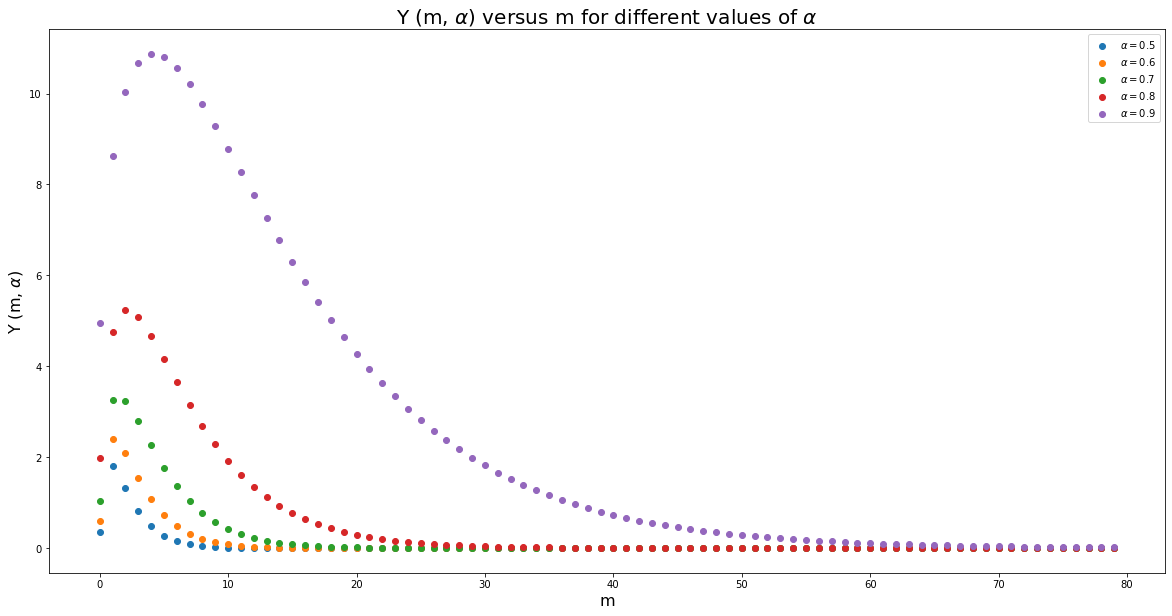
\includegraphics[width=1.0\linewidth]{image.png}
    \caption{A numerical plot showing trends for $\Upsilon(m,\alpha)$ versus m, for varying values of \alpha.}
    \label{fig:enter-label}
\end{figure}











\subsubsection{Sample Wave-fitting Routine and Parameters}

To simplify the theoretical model for use in our wave-fitting routine, we revise the aforesaid equations. Recall that,
\begin{equation}
    y(x) = a\left(\frac{x-x_{r}}{x_{f}}\right)e^{-\frac{(|x-x_{r}|)^{3}}{(x_{d}x_{f})^{3}}}\cos\left[\phi_{0} - \frac{3\pi}{4} - \frac{{(x-x_{r})^2}}{{x_{f}^{2}}}\right]\zeta\left(\frac{x-x_{r}}{x_{f}}\right).
\end{equation}
Let $\mathcal{A} = \frac{a}{x_{f}}$ and $y_{d} = x_{d}x_{f}$. The wave-fit equation becomes:
\begin{equation}
    y(x) = \mathcal{A}(x-x_{r})e^{-\frac{(|x-x_{r}|)^{3}}{(y_{d})^{3}}}\cos\left[\phi_{0} - \frac{3\pi}{4} - \frac{{(x-x_{r})^2}}{{x_{f}^{2}}}\right]\zeta(\frac{x-x_{r}}{x_{f}}).
\end{equation}

When implemented, the aforesaid operation simply produces $\mathcal{A}$, $y_{d}$, $\phi_{0}$, $x_{r}$ and $x_{f}$ as the wave-fit parameters. Further operation decomposes $\mathcal{A}$ and $y_{d}$ to give rise to the dimensionless amplitude, $a$, and the damping parameter, $x_{d}$. 

\vspace{3}

\textbf{Note:}

\vspace{3}
\textbf{$a$} = Dimensionless amplitude for the density wave-fit.

\vspace{3}
\textbf{$x_{d}$} = Damping parameter for the specific density wave.

\vspace{3}
\textbf{$\phi_{0}$} = Initial phase value from the wave-fit routine (in radian).

\vspace{3}
\textbf{$x_{r}$} = Wave-fit for the resonant radius of the wave (in Kilometer).

\vspace{3}
\textbf{$x_{f}$} = Winding parameter.

\vspace{10}
The attached figure illustrates the juxtaposition of two plots: one for the actual dataset from Cassini VIMS (indicated by the blue legend), and the other for the linear density wave-fitting model mentioned earlier (designated by the black legend). The vertical axis corresponds to the normalized optical depth for the section of the ring where the spiral density wave was detected by Cassini VIMS, while the horizontal axis represents the radial offset in relation to the planet's center.
The necessary dimensionless parameters, including amplitude, damping, and winding, are extracted. Initially, we calculate the surface mass density using the winding parameter and subsequently derive the required viscosity. Finally, we convert the dimensionless amplitude of the spiral density wave into the necessary amplitude for the normal-mode oscillation within Saturn's interior that induced such a wave in that specific segment of Saturn's C-ring.
The errors in these measurements for all wave signals are estimated through the conventional bootstrapping technique, which we will describe in the following section.


\begin{figure}[h]
\centering 
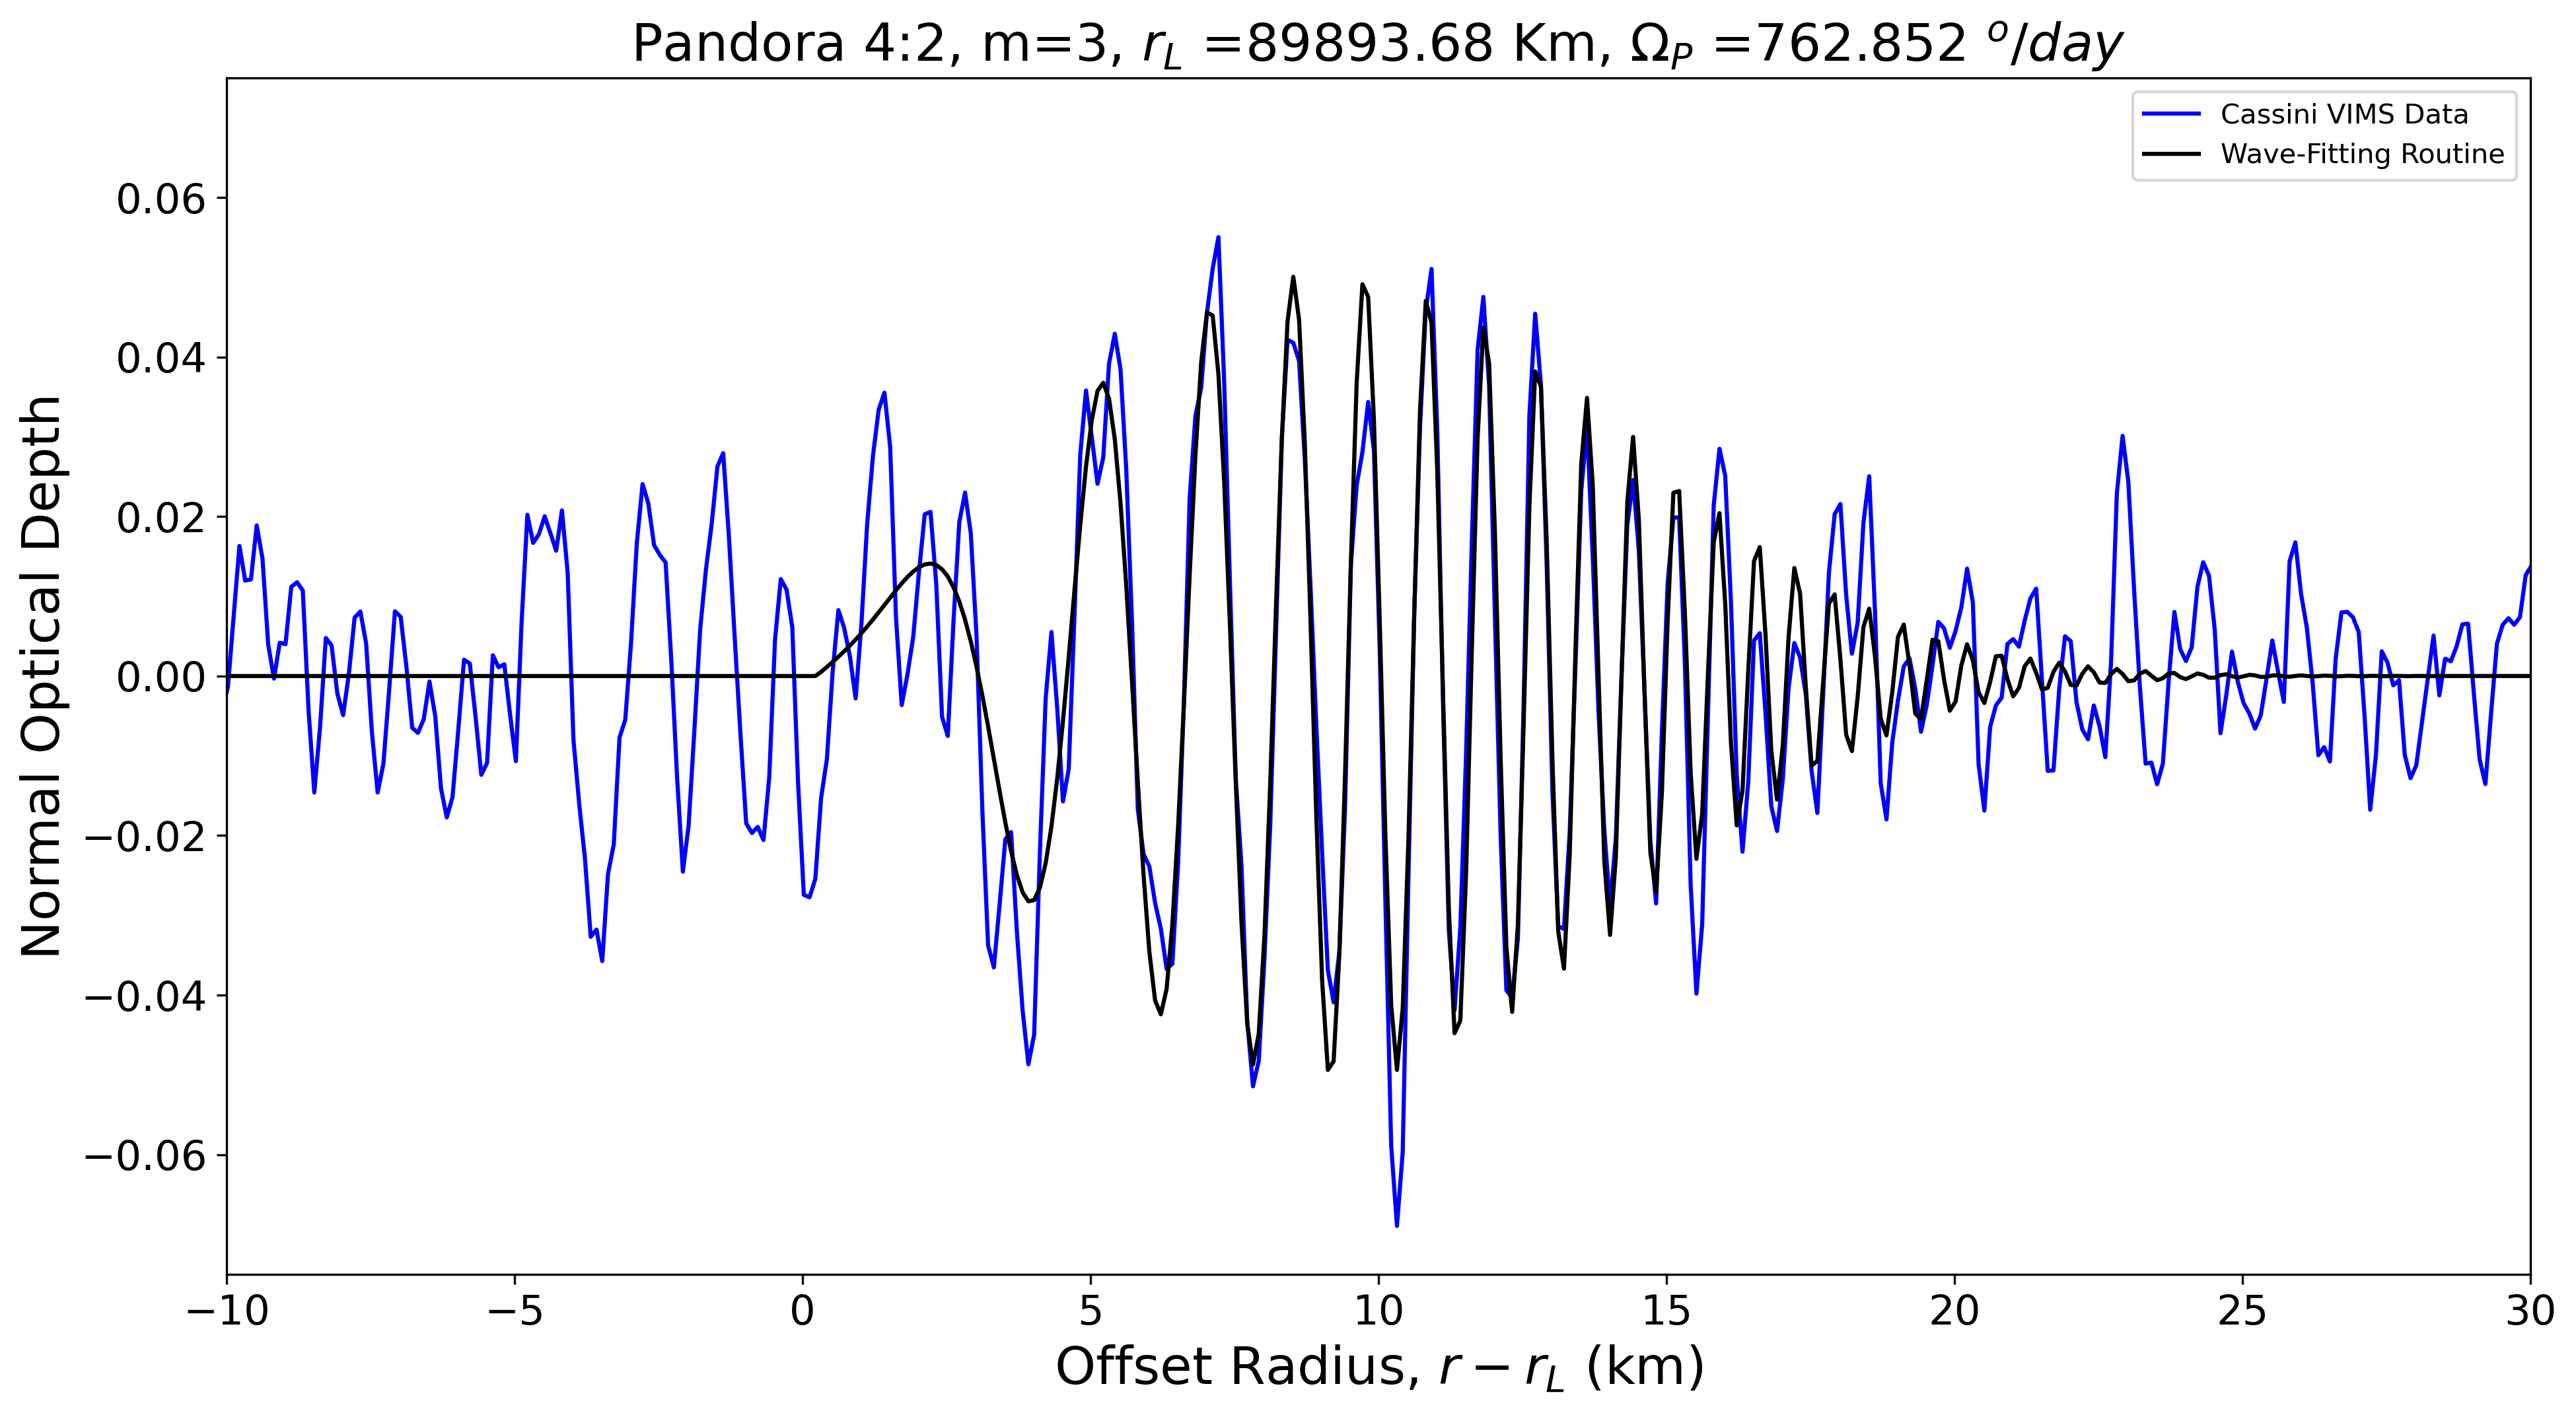
\includegraphics[width=0.9\textwidth]{pandora_42_wavefit.png} 
\caption{A wave-fitting routine for the Pandora 4:2 Satellite resonance..} \label{fig:my_label}
\end{figure}



\begin{table}
\centering
\begin{tabular}{|c|c|c|}
\hline
\textbf{Nomenclature} & \textbf{Symbol} & \textbf{Value} \\
\hline
Resonance label & $m$ & 3 \\
\hline
Resonance location & $r_{L}$ & 89893.68 Km \\
\hline
Pattern speed & $\Omega_{p}$ & 762.852 $^{o}/day$ \\
\hline
Amplitude & a & 0.0074 \\
\hline
Damping Length & $x_{d}$ & 6.9140 \\
\hline
Initial Phase & $\phi_{0}$ & -3.2364 rad \\
\hline
Resonance Offset & $x_{r}$ & 0.2341 Km \\
\hline
Winding Parameter & $x_{f}$ & 1.8745 Km \\
\hline
\end{tabular}
\caption{Parameter values for wave-fitting routine for W84.64}
\end{table}






%are extracted from the routine, as  ( $a$, $x_{d}$, $x_{f}$ and $\sigma_{0}$). These parameters are then used in the required expressions above, to generate the given plots in the next section. 

%......................................................................................
\subsubsection{Error Analysis for Independent Parameters: Bootstrap Resampling}

Since each density wave profile comprises a series of occultations, there is a requirement for a precise yet efficient method to quantify uncertainties or variations in the (independent) parameters resulting from the wave-fitting routine for each wave signal. Therefore, there is a necessity for bootstrap resampling.

Bootstrap resampling is a powerful statistical technique that involves drawing multiple samples with replacement from the observed data to simulate a distribution of parameter values or estimate the uncertainty or variability in a parameter without relying on assumptions about the underlying population distribution\cite{Chernick2007BootstrapMA}\cite{davison_hinkley_1997}. By repetitively resampling the data, we can generate a range of potential parameter sets, allowing us to assess the robustness and reliability of the fitted wave profiles. That way we tend to capture the inherent variability in the data and provide a more comprehensive understanding of the uncertainties associated with the density wave parameters\cite{Efron1994AnIT}\cite{article}. This method is particularly useful for error analysis in measurements. The following steps outline the process along with relevant equations:

\paragraph{Generate Resampled Datasets:}
Let $\mathbf{X} = \{x_1, x_2, \ldots, x_n\}$ represent the original dataset with $n$ measurements of a parameter (e.g., density). To perform bootstrap resampling, generate a large number of resampled datasets, denoted as $\mathbf{X}^{*}_1, \mathbf{X}^{*}_2, \ldots, \mathbf{X}^{*}_B$, each with the same size as the original dataset ($n$). Resampling is done by randomly sampling, with replacement, from the original dataset\cite{Chernick2007BootstrapMA}\cite{davison_hinkley_1997}\cite{Efron1994AnIT}\cite{article}:
\begin{equation}
\mathbf{X}^{*}_b = \{x^{*}_{b1}, x^{*}_{b2}, \ldots, x^{*}_{bn}\}, \quad b = 1, 2, \ldots, B
\end{equation}

\paragraph{Compute the Parameter of Interest:}
For each resampled dataset $\mathbf{X}^{*}_b$, where $b = 1, 2, \ldots, B$, calculate the parameter of interest, denoted as $\theta$. For example, if the interest is in the mean, the parameter estimate for the $b$th resampled dataset, denoted as $\theta^{*}_{b}$, is calculated as\cite{Chernick2007BootstrapMA}\cite{davison_hinkley_1997}\cite{Efron1994AnIT}\cite{article}:
\begin{equation}
\theta^{*}_{b} = g(\mathbf{X}^{*}_b),
\end{equation}
where $g(.)$ represents the function or statistic used to calculate the parameter estimate.
\paragraph{Calculate Variability:}
After obtaining the parameter estimates $\theta^{*}_{1}, \theta^{*}_{2}, \ldots, \theta^{*}_{B}$ for all resampled datasets, analyze the distribution of these estimates to determine variability. Calculate the mean estimate ($\bar{\theta}^{*}$) and standard deviation estimate ($s^{*}$) as follows\cite{Chernick2007BootstrapMA}\cite{Efron1994AnIT}:
\begin{equation}
\bar{\theta}^{*} = \frac{1}{B}\sum_{b=1}^{B}\theta^{*}_{b},
\end{equation}

\begin{equation}
s^{*} = \sqrt{\frac{1}{B-1}\sum_{b=1}^{B}(\theta^{*}_{b} - \bar{\theta}^{*})^2}
\end{equation}

We can compute the standard error ($SE$) using the given expression\cite{Chernick2007BootstrapMA}\cite{davison_hinkley_1997}\cite{Efron1994AnIT}:

\begin{equation}
SE = \frac{s^{*}}{\sqrt{B}},
\end{equation}
and apply the aforesaid operations to our work.

%\begin{equation}
%\text{Confidence interval} = \left[\bar{\theta}^{*} - z \cdot SE, \bar{\theta}^{*} + z \cdot SE\right]
%\end{equation}

%where $z$ 

\paragraph{Interpret the Results:}
Based on the distribution of the parameter estimates, express the uncertainty in the measurement. Report the mean value and provide a confidence interval, which gives a range within which the true parameter value is likely to fall. Bootstrap resampling allows for estimating the sampling variability of a parameter without assuming a specific distribution, providing a robust method for error analysis in measurements. In essence, bootstrap resampling serves as a powerful tool for refining our analyses and ensuring that the derived parameters are not overly sensitive to specific data points, contributing to a more robust and reliable characterization of density wave profiles.

%......................................................................................
\subsubsection{Error Analysis for Dependent Parameters: Method of Propagation}
In scientific and engineering applications, it is common to encounter functions of multiple variables where each variable has associated uncertainties. Understanding how uncertainties propagate through these functions is crucial for assessing the reliability of results. In this section, we explore the error propagation formula, beginning with the general case where variables may be correlated. We leverage the Taylor series expansion and properties of covariance matrices to derive a comprehensive expression for the uncertainty in a function. Additionally, we simplify this expression in the special case where variables are uncorrelated, providing a more practical and computationally efficient formula.

%We start by invoking the Taylor series expansion to express a function \( f(\mathbf{x}) \) as a sum of partial derivatives around a specific point \( \mathbf{x}_0 \). This allows us to derive the differential of \( f \) and subsequently formulate the error propagation formula. In the general case, we account for correlations between variables through the covariance matrix.

%When variables are uncorrelated, the error propagation formula simplifies, making the computation more straightforward. We explore this special case, providing a simplified expression that is often used in practice.

Deriving the error propagation formula from Taylor's theorem for a general case with \( n \) variables \( x_1, x_2, \ldots, x_n \) and a function \( w = f(x_1, x_2, \ldots, x_n) \), Taylor's theorem for a multivariable function is given by\cite{taylor2022introduction}\cite{LUO201723}:
\begin{equation}
f(x_1 + \Delta x_1, x_2 + \Delta x_2, \ldots, x_n + \Delta x_n) \approx f(x_1, x_2, \ldots, x_n) + \sum_{i=1}^{n} \frac{\partial f}{\partial x_i} \Delta x_i
\end{equation}

Now, consider the function \( w = f(x_1, x_2, \ldots, x_n) \) and introduce uncertainties:
\begin{equation}
w(x_1 + \Delta x_1, x_2 + \Delta x_2, \ldots, x_n + \Delta x_n) \approx w(x_1, x_2, \ldots, x_n) + \sum_{i=1}^{n} \frac{\partial w}{\partial x_i} \Delta x_i
\end{equation}

Now, square both sides:
\begin{equation}
(w + \Delta w)^2 \approx w^2 + 2w\Delta w + (\Delta w)^2
\end{equation}

Taking the expectation and neglecting higher-order terms:
\begin{equation}
\langle (\Delta w)^2 \rangle \approx \sum_{i=1}^{n} \langle \left(\frac{\partial w}{\partial x_i}\right)^2 \rangle \langle (\Delta x_i)^2 \rangle + 2 \sum_{i=1}^{n} \sum_{j=i+1}^{n} \langle \frac{\partial w}{\partial x_i} \frac{\partial w}{\partial x_j} \rangle \langle \Delta x_i \Delta x_j \rangle
\end{equation}

Here, \( \langle \cdot \rangle \) denotes the expectation value.

The covariance terms (\( \text{Cov}(x_i, x_j) \)) are introduced in the correlation terms:
\begin{equation}
\langle \Delta x_i \Delta x_j \rangle = \text{Cov}(x_i, x_j)
\end{equation}

Now, we can rewrite the expression:
\begin{equation}
\langle (\Delta w)^2 \rangle \approx \sum_{i=1}^{n} \langle \left(\frac{\partial w}{\partial x_i}\right)^2 \rangle \langle (\Delta x_i)^2 \rangle + 2 \sum_{i=1}^{n} \sum_{j=i+1}^{n} \langle \frac{\partial w}{\partial x_i} \frac{\partial w}{\partial x_j} \rangle \text{Cov}(x_i, x_j)
\end{equation}

Finally, dividing both sides by \(w^2\) and taking the square root, we get the error propagation formula with correlation for \( n \) variables\cite{articleb}\cite{taylor2022introduction}\cite{weisstein2000error}\cite{LUO201723}:
\begin{equation}
\frac{\sigma_w}{w} \approx \sqrt{\sum_{i=1}^{n} \left(\frac{\partial w}{\partial x_i}\right)^2 \left(\frac{\sigma_{x_i}}{x_i}\right)^2 + 2 \sum_{i=1}^{n} \sum_{j=i+1}^{n} \frac{\partial w}{\partial x_i} \frac{\partial w}{\partial x_j} \frac{\text{Cov}(x_i, x_j)}{x_i x_j}}
\end{equation}

This formula accounts for both the individual uncertainties in each variable (\( \frac{\sigma_{x_i}}{x_i} \)) and the correlations between different pairs of variables (\( \text{Cov}(x_i, x_j) \)). For the case of non-correlation, where all covariance terms are zero, ($\(\text{Cov}(x_i, x_j) \) = 0 \forall i \neq j$), the formula simplifies to the standard error propagation formula:
\begin{equation}
\frac{\sigma_w}{w} \approx \sqrt{\sum_{i=1}^{n} \left(\frac{\partial w}{\partial x_i}\right)^2 \left(\frac{\sigma_{x_i}}{x_i}\right)^2}
\end{equation}

Examining the spread of errors through differential calculus proves effective for models defined by smooth and differentiable relationships. This method offers valuable insights into error propagation and uncertainty, particularly in compact theoretical models. It establishes a conceptual framework for understanding how variability moves through complex systems of equations\cite{articleb}. However, limitations exist. The approach assumes differentiability, making it unsuitable for models with discontinuities, step functions, or conditional logic. Additionally, it is inherently local, disregarding higher-order terms and lacking information on outliers\cite{articleb}. Variance-based error analysis assumes a symmetric distribution, limiting its applicability to skewed distributions like the log-normal distribution\cite{MCKAY199944}. Despite these drawbacks, the differential analysis remains a valuable guide for comprehending uncertainty propagation in predictive models\cite{articleb}\cite{taylor2022introduction}\cite{LUO201723}.
%......................................................................................

\subsubsection{Discussions on Model Parameters For the Wave-Fit Procedures:}

Actually, there is no one-size-fits-all reason for why we chose to include the fitting parameters described above in our theoretical model. It was an essential power-play to enable us to strike a balance between the complexity of the theoretical model and the need to accurately capture the underlying behavior of the data. Our decision was guided by a combination of several factors with their succinct descriptions below.

1. \textbf{Generalization:} The goal of modeling is often to make predictions or inferences on new, unseen data. Models with too many parameters may fit the training data extremely well but fail to generalize to new data. Reducing the number of parameters can lead to models that generalize better \cite{james2013introduction}.

2. \textbf{Quality of Data:} High-quality, precise data can often support more complex models with more parameters. Since our data has some traces of noise, using a simpler model with fewer parameters might be more appropriate to avoid overfitting \cite{bishop2006pattern}.

3. \textbf{Overfitting:} Overfitting is a common concern when fitting non-linear models with a large number of parameters to non-linear data. Overfitting occurs when the model captures noise and fluctuations in the data rather than the underlying trend or pattern. Reducing the number of parameters helps prevent overfitting by making the model less complex and more robust to noise \cite{bishop2006pattern}.

4. \textbf{Interpretability:} Non-linear models with a high number of parameters can be challenging to interpret. By reducing the number of parameters, we can make the model more interpretable, as it becomes easier to understand the functional relationships between input variables and the model's predictions \cite{molnar2020interpretable}.

5. \textbf{Computational Efficiency:} Fitting non-linear models with a large number of parameters can be computationally intensive and time-consuming. Reducing the parameter space makes the optimization problem more tractable and faster to converge using tools like SciPy \cite{nocedal2006numerical}.

6. \textbf{Stability:} Non-linear regression can be sensitive to the initial parameter values, and models with a high number of parameters may have multiple local minima in the objective function (like degeneracies in the wave-fit parameters). Reducing the number of parameters can make the optimization process more stable and less prone to getting stuck in local optima \cite{nocedal2006numerical}.

7. \textbf{Bias-Variance Trade-off:} Non-linear models with many parameters are prone to having high variance, which can lead to unpredictable and erratic behavior. Reducing the number of parameters can reduce model variance and improve its reliability \cite{hastie2009elements}.

8. \textbf{Data Requirements:} Fitting complex non-linear models with numerous parameters often requires a substantial amount of data to estimate those parameters accurately. Since we are working with aliquot amount of Cassini VIMS dataset, reducing the number of parameters can help prevent overfitting and lead to more stable and trustworthy estimates.

9. \textbf{Occam's Razor:} Ceteris paribus, this principle suggests that simpler explanations (or models) should be preferred to their complex versions. In many cases, a simpler model with fewer parameters is preferred, provided it can adequately describe the trend of dataset involved. It is easier to interpret and generalize a simple model, as opposed to a complex model \cite{Sober2015-SOBORA}.





\subsection{Preliminary Result I}
In this section, we feature the predicted gravitational potential estimate results for satellite spiral density waves, as well as the computed estimates of gravitational potentials gotten through the aforementioned techniques. 

\subsubsection{Satellite Waves: Predicted Estimates for Gravitational Potential}
Starting with the satellite wave, we present the given table containing predicted values for the respective gravitational potentials, using the normalized torque expression for equation (61) from \cite{Hedman_2022}:
\begin{equation}
    \Psi_{m}^{'} = \sqrt{\frac{3|m - 1|n_{L}^{2}}{m\pi^{2}} \left|\frac{\mathcal{T}}{\sigma_{0}}\right|},
\end{equation}
where $n_{L}^{2} = \frac{G M_{P}}{r_{L}^{3}}$.


\begin{table}
\centering
\begin{tabular}{lllll}
\hline
Resonance Name & $m$ & $r_{L}$ (Km) & $\mathcal{T}/\sigma_{0}$ (Km$^{4}$s$^{-2}$) & $\Psi_{m}^{'} (m^{2}s^{-2})$ \\
\hline
Mimas 4:1 & 2 & 74890.067 & -8.987453e-08 & 0.035125 \\
Pan 2:1 & 2 & 85105.021 & -2.971890e-09 & 0.005273 \\
Atlas 2:1 & 2 & 87645.684 & -5.346249e-09 & 0.006767 \\
Prometheus 4:2 & 3 & 88434.120 & -2.651270e-10 & 0.001717 \\
Mimas 6:2 & 3 & 89883.135 & -9.726598e-10 & 0.003209 \\
Pandora 4:2 & 3 & 89893.680 & -7.171256e-10 & 0.002755 \\
\hline
\end{tabular}
\caption{Predicted data for spiral density waves excited by Saturn's Satellite resonances.}
\end{table}




\subsubsection{Satellite Waves: Parameters from Wave-fitting Routine}

%..................................................................................

%..................................................................................

\begin{figure}[h]
    \centering

    \begin{subfigure}{0.35\linewidth}
        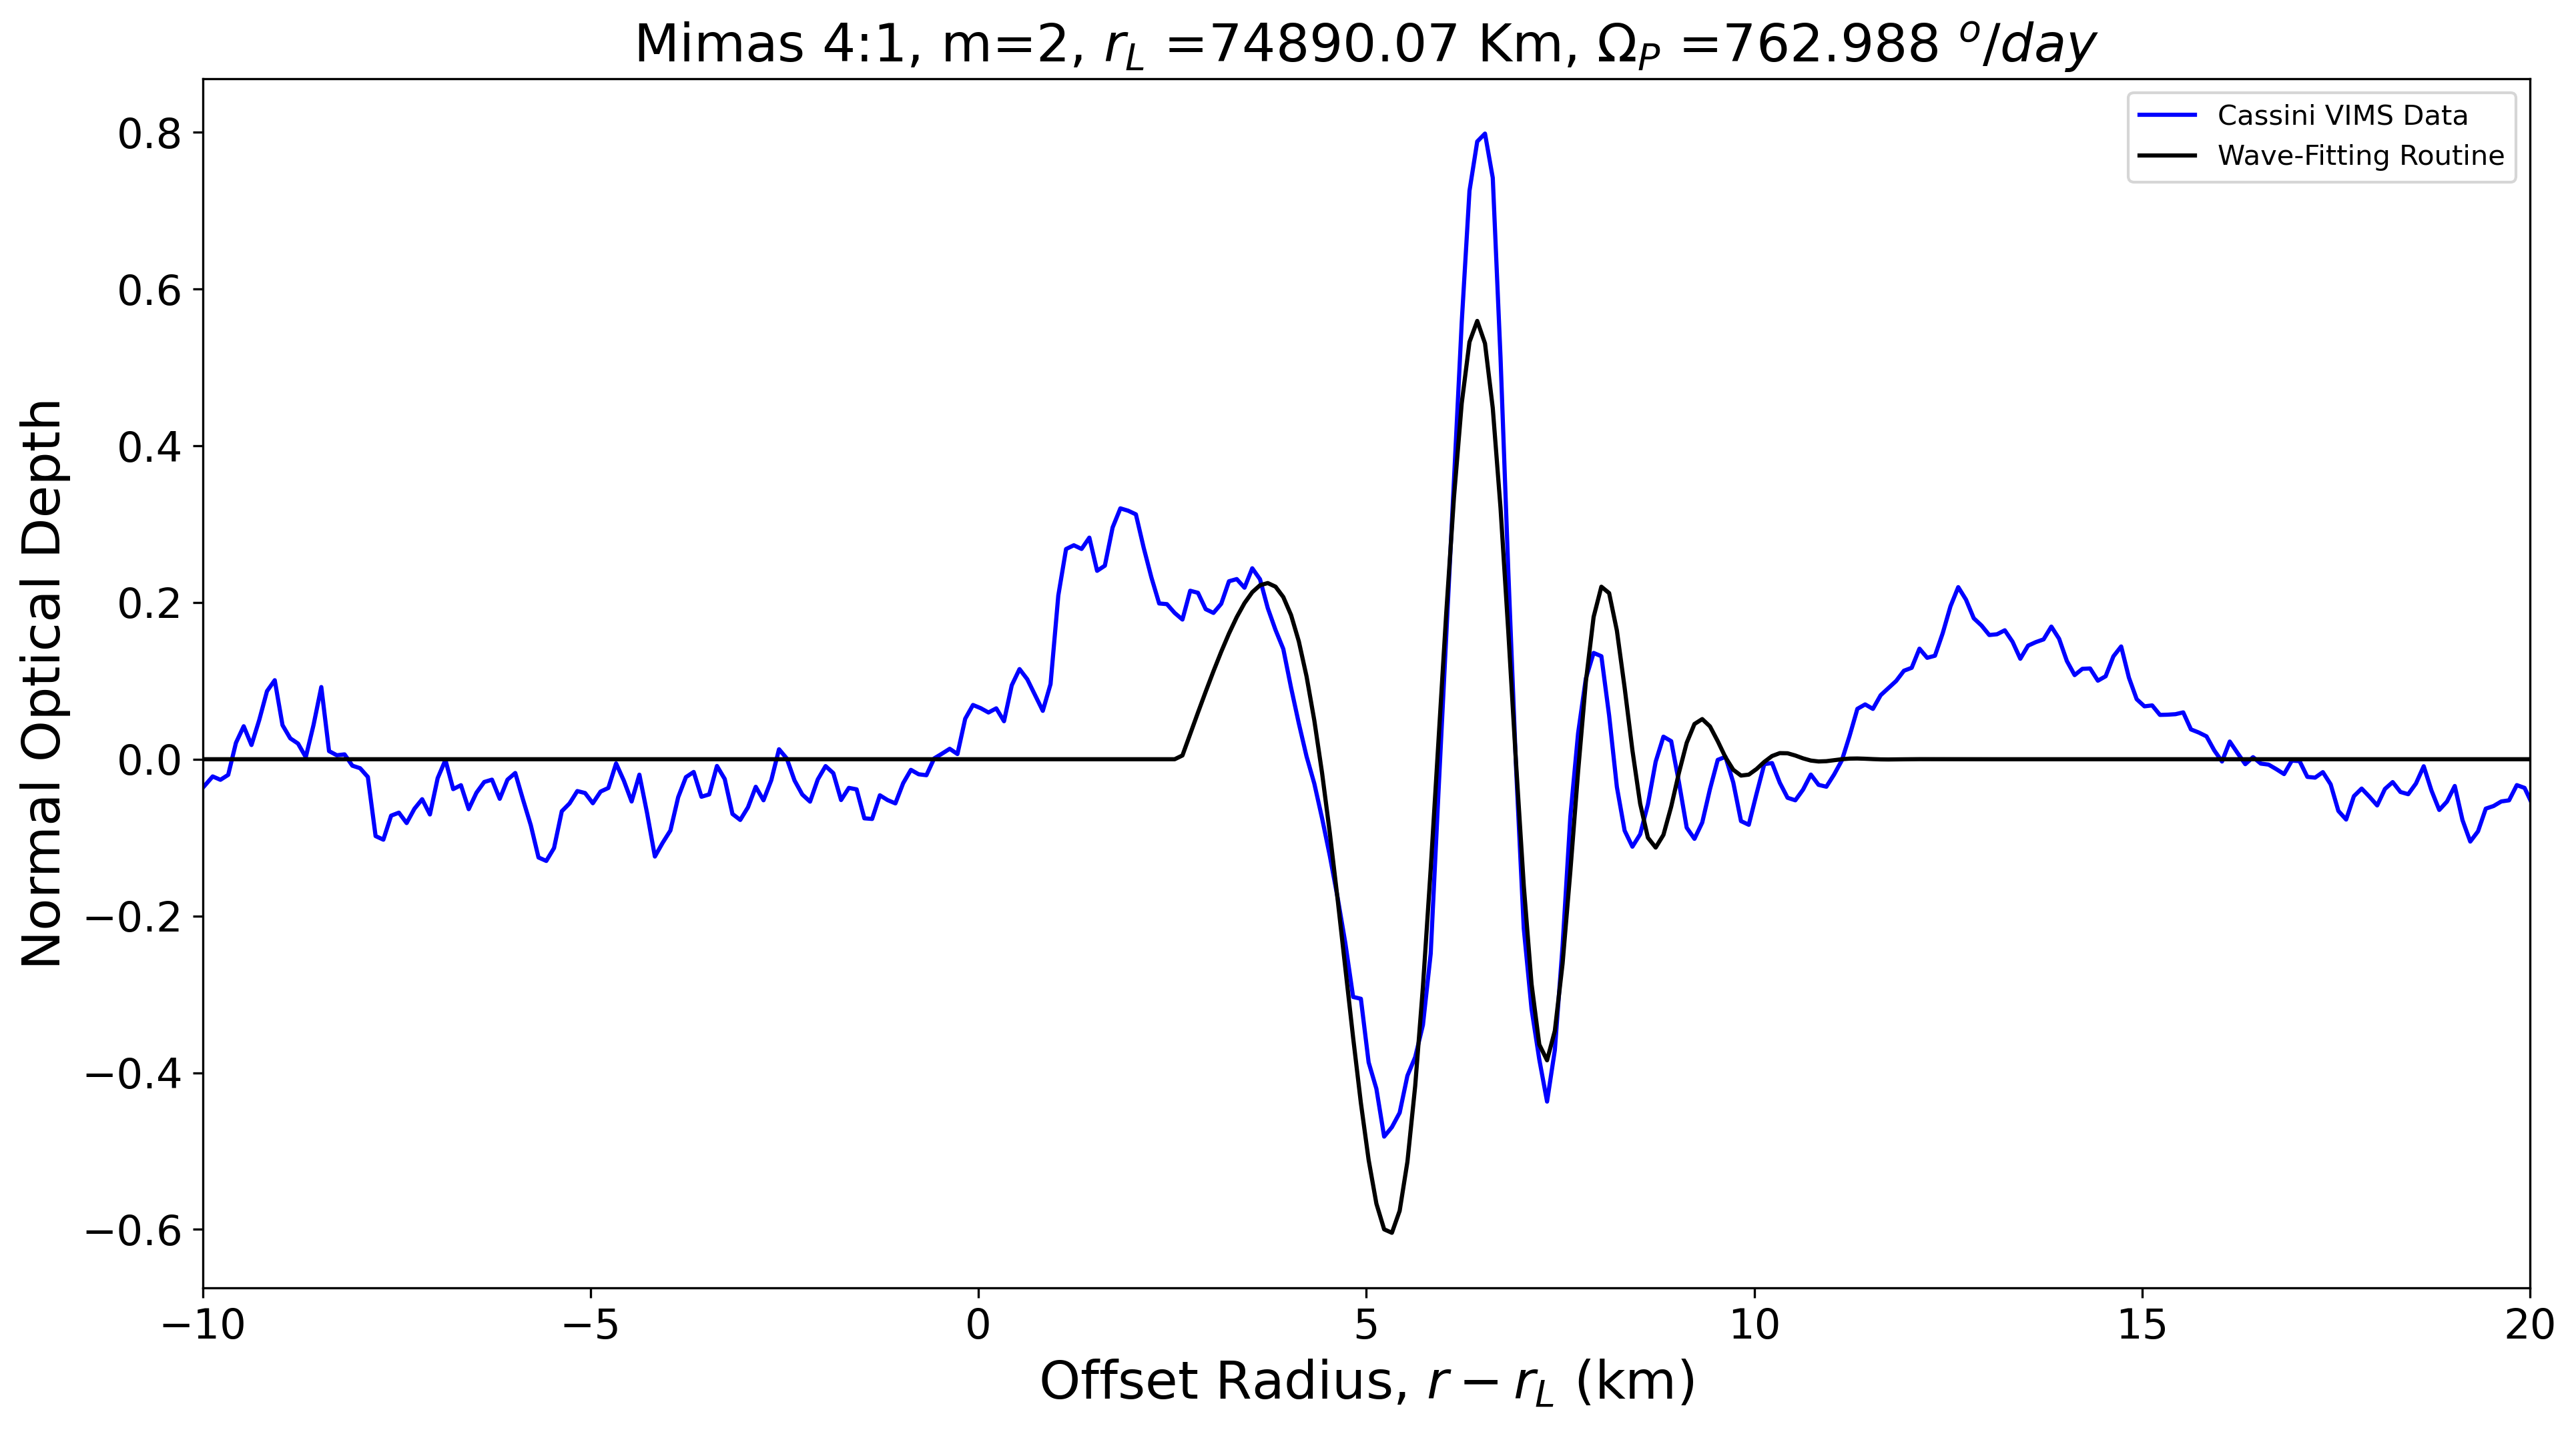
\includegraphics[width=\linewidth]{mimas41_wavefit.png}
        %\caption{Caption for Mimas41}
        \label{fig:mimas41}
    \end{subfigure}
    \hspace{1\linewidth} % Adjust the horizontal space between subfigures

    \begin{subfigure}{0.35\linewidth}
        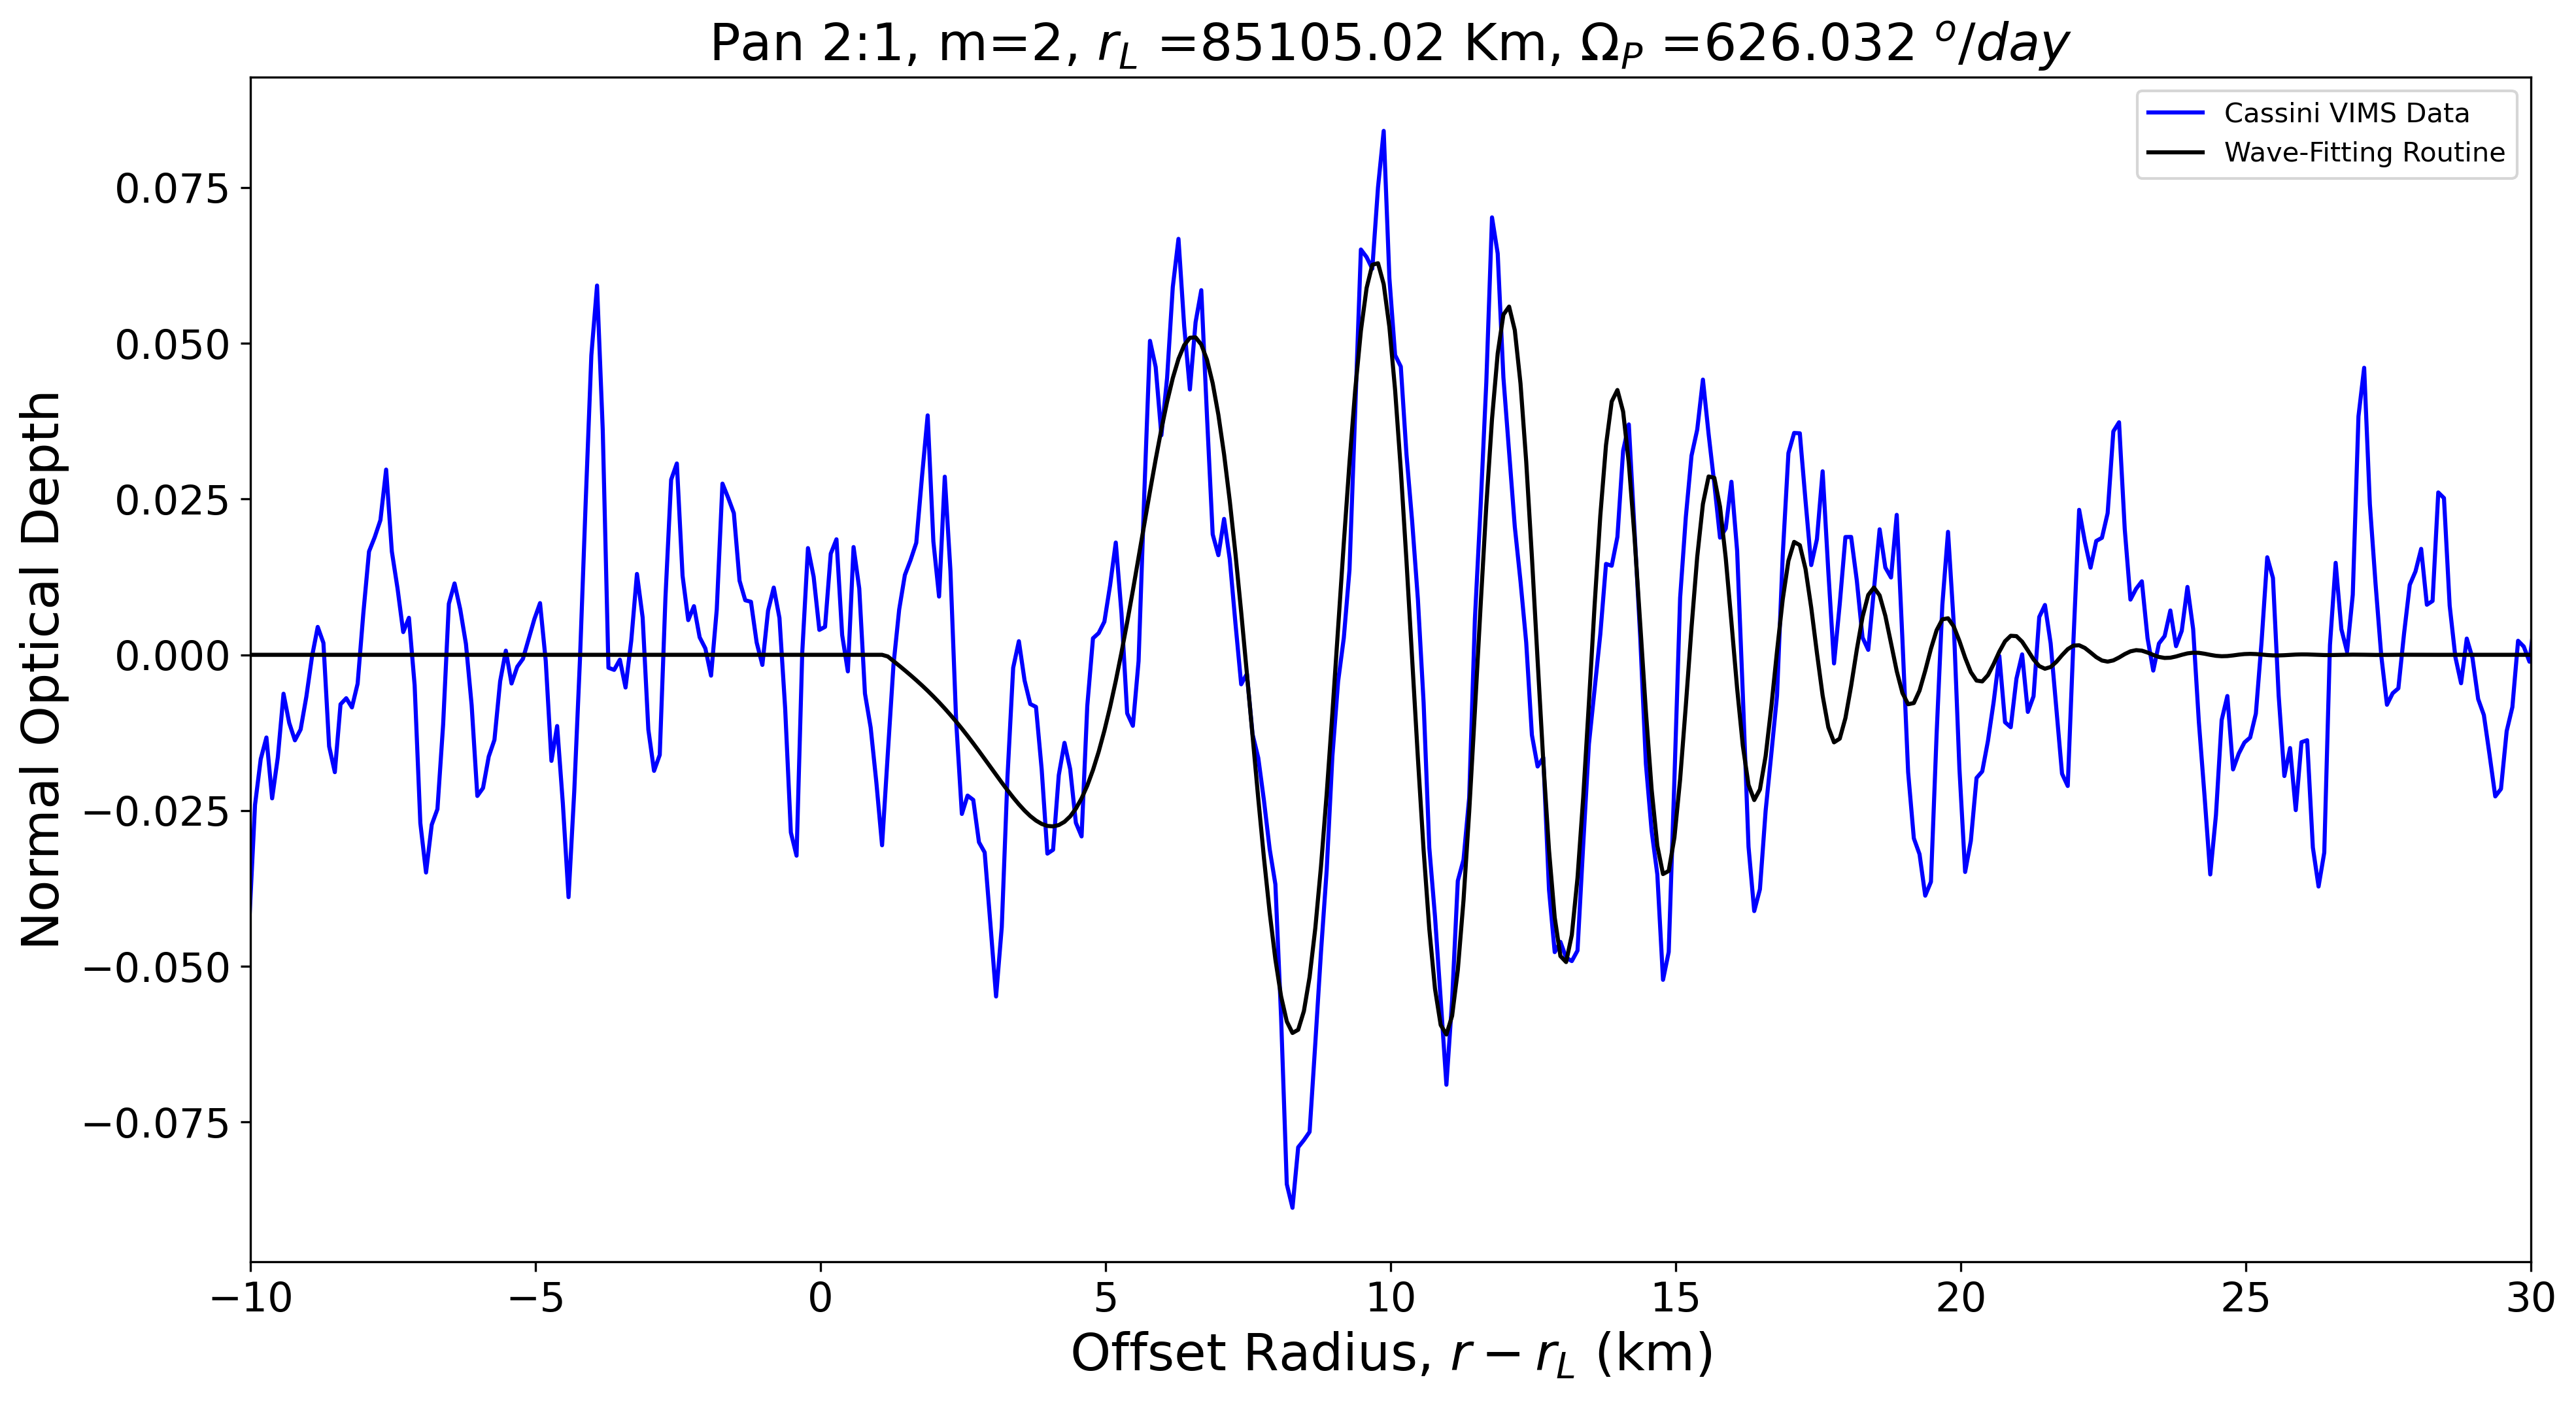
\includegraphics[width=\linewidth]{pan_21_wavefit.png}
        %\caption{Caption for Pan21}
        \label{fig:pan21}
    \end{subfigure}
    \hspace{1\linewidth}

    \begin{subfigure}{0.35\linewidth}
        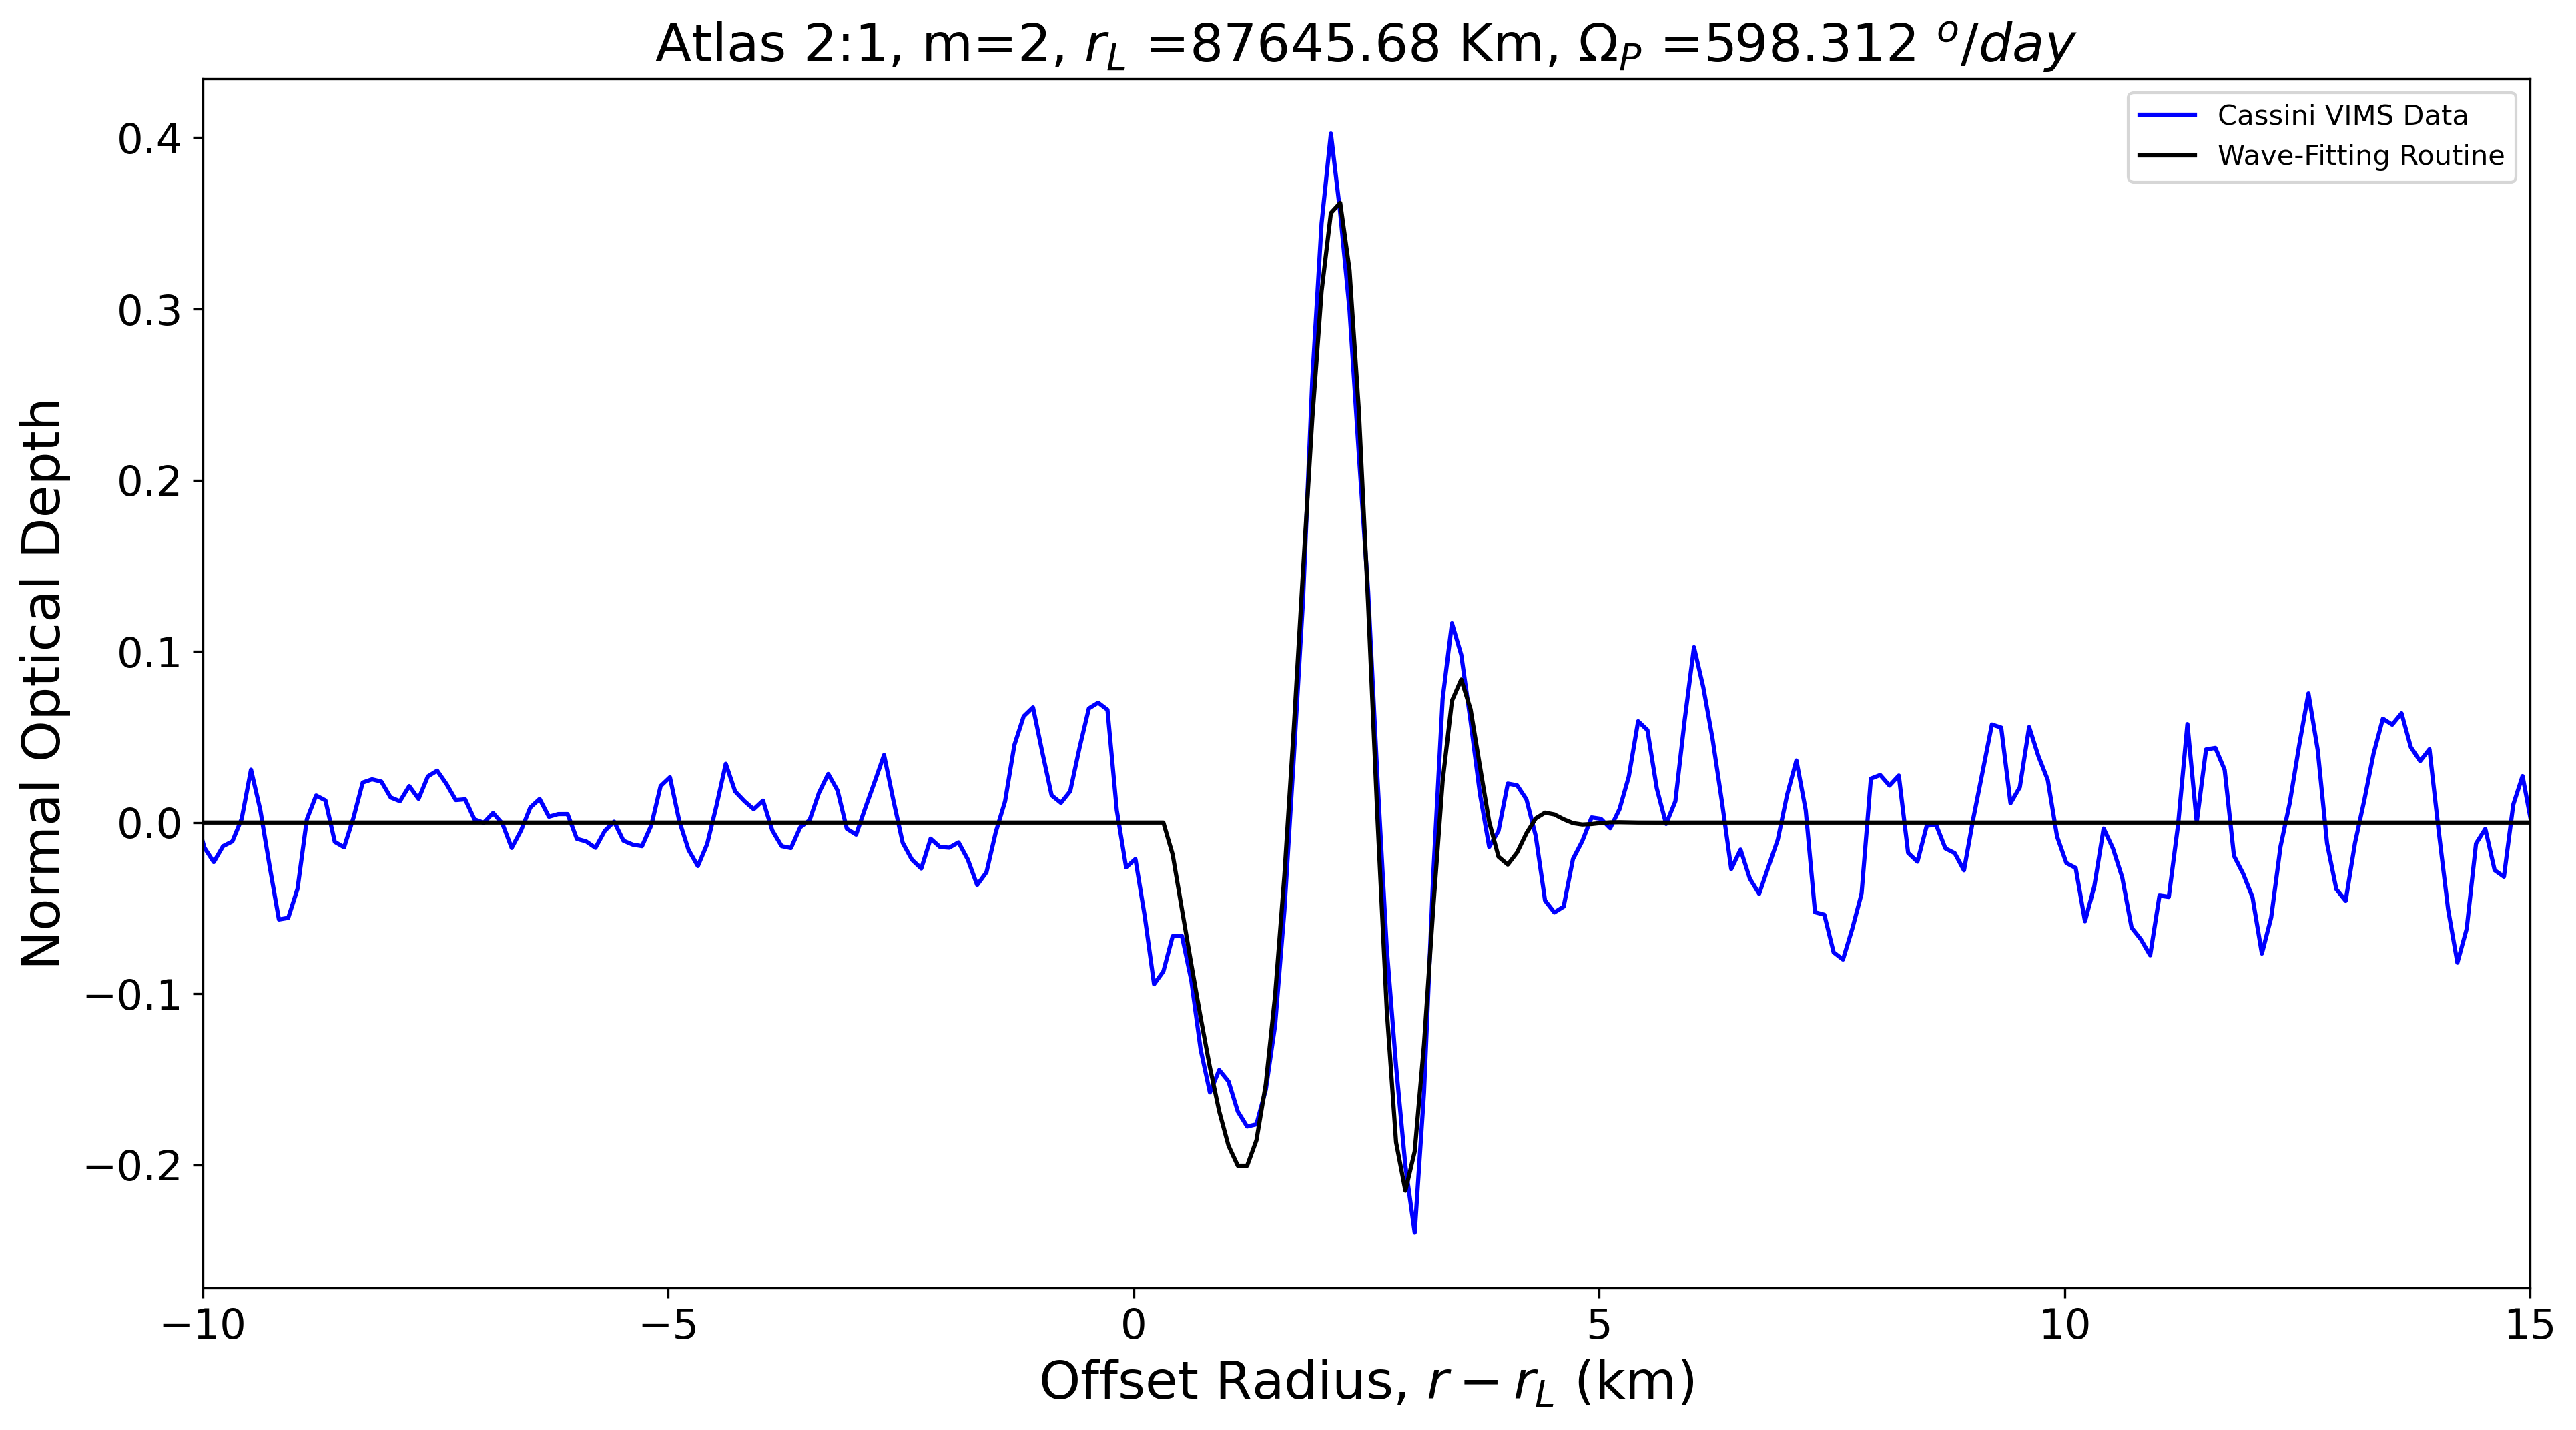
\includegraphics[width=\linewidth]{atlas_21_wavefit.png}
        %\caption{Caption for Atlas21}
        \label{fig:atlas21}
    \end{subfigure}
    \\ % Start a new line for the next row of subfigures

    \begin{subfigure}{0.35\linewidth}
        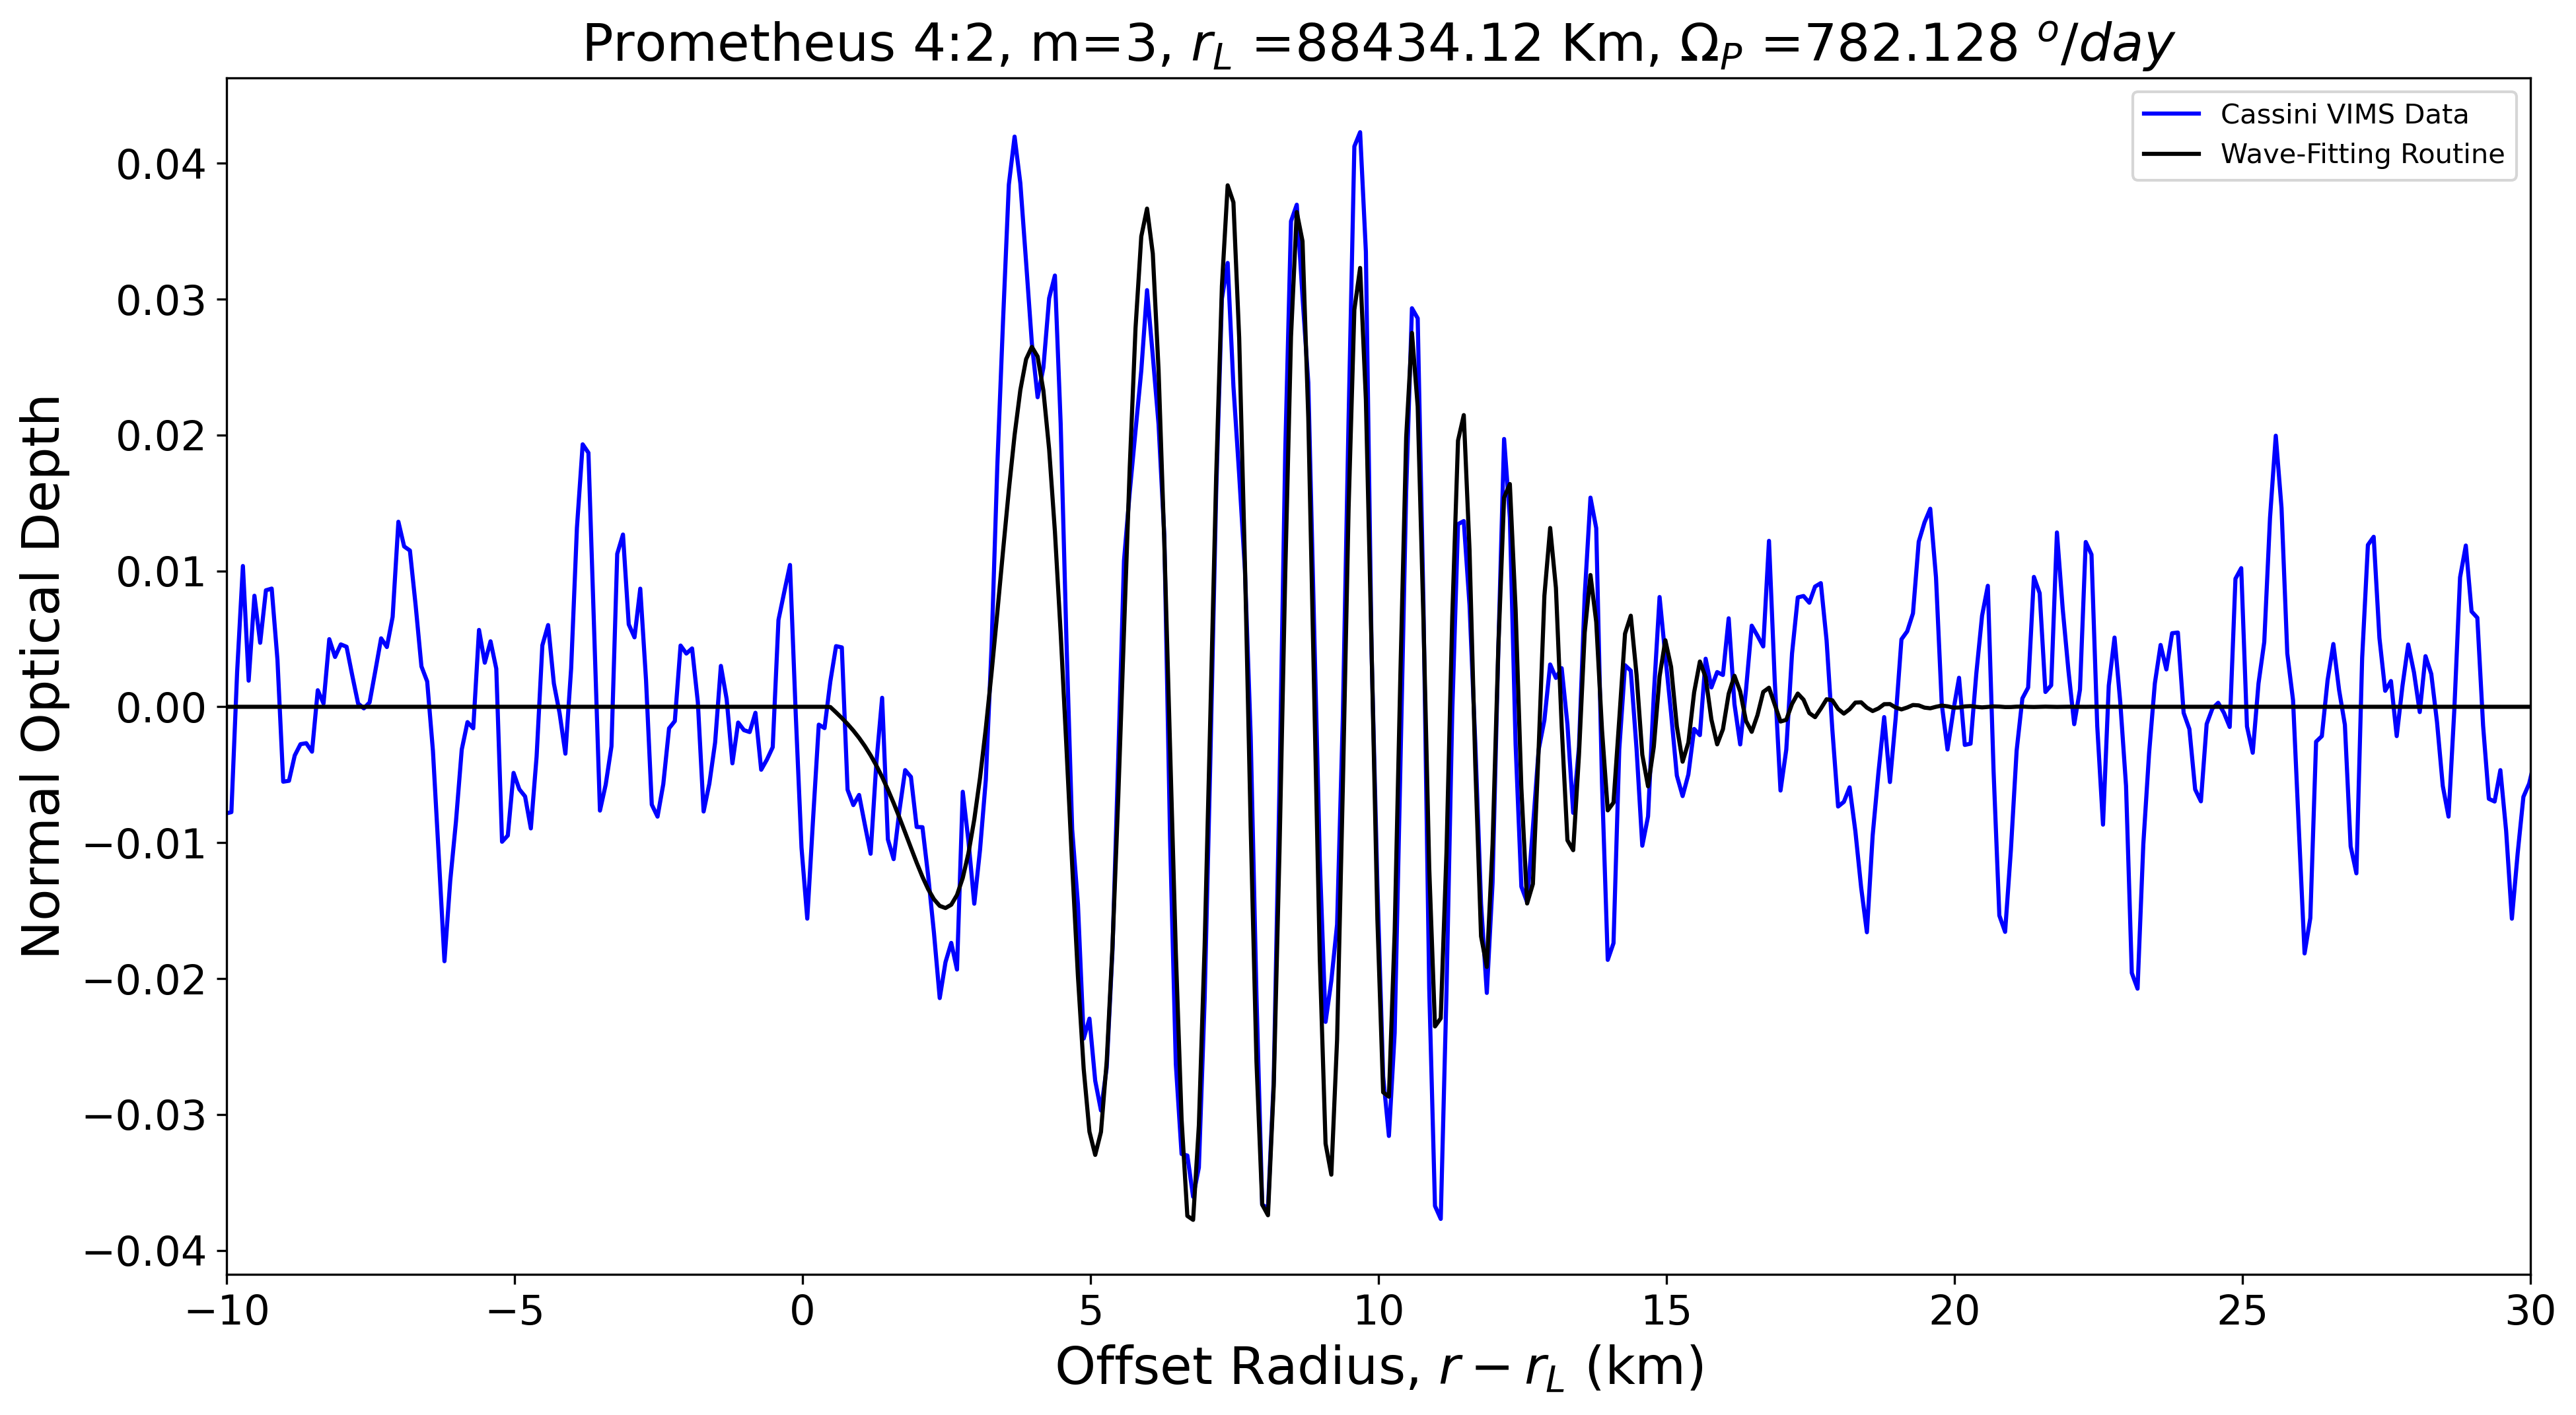
\includegraphics[width=\linewidth]{prometheus_42_wavefit.png}
        %\caption{Caption for Prometheus42}
        \label{fig:prometheus42}
    \end{subfigure}
    \hspace{1\linewidth}

    \begin{subfigure}{0.35\linewidth}
        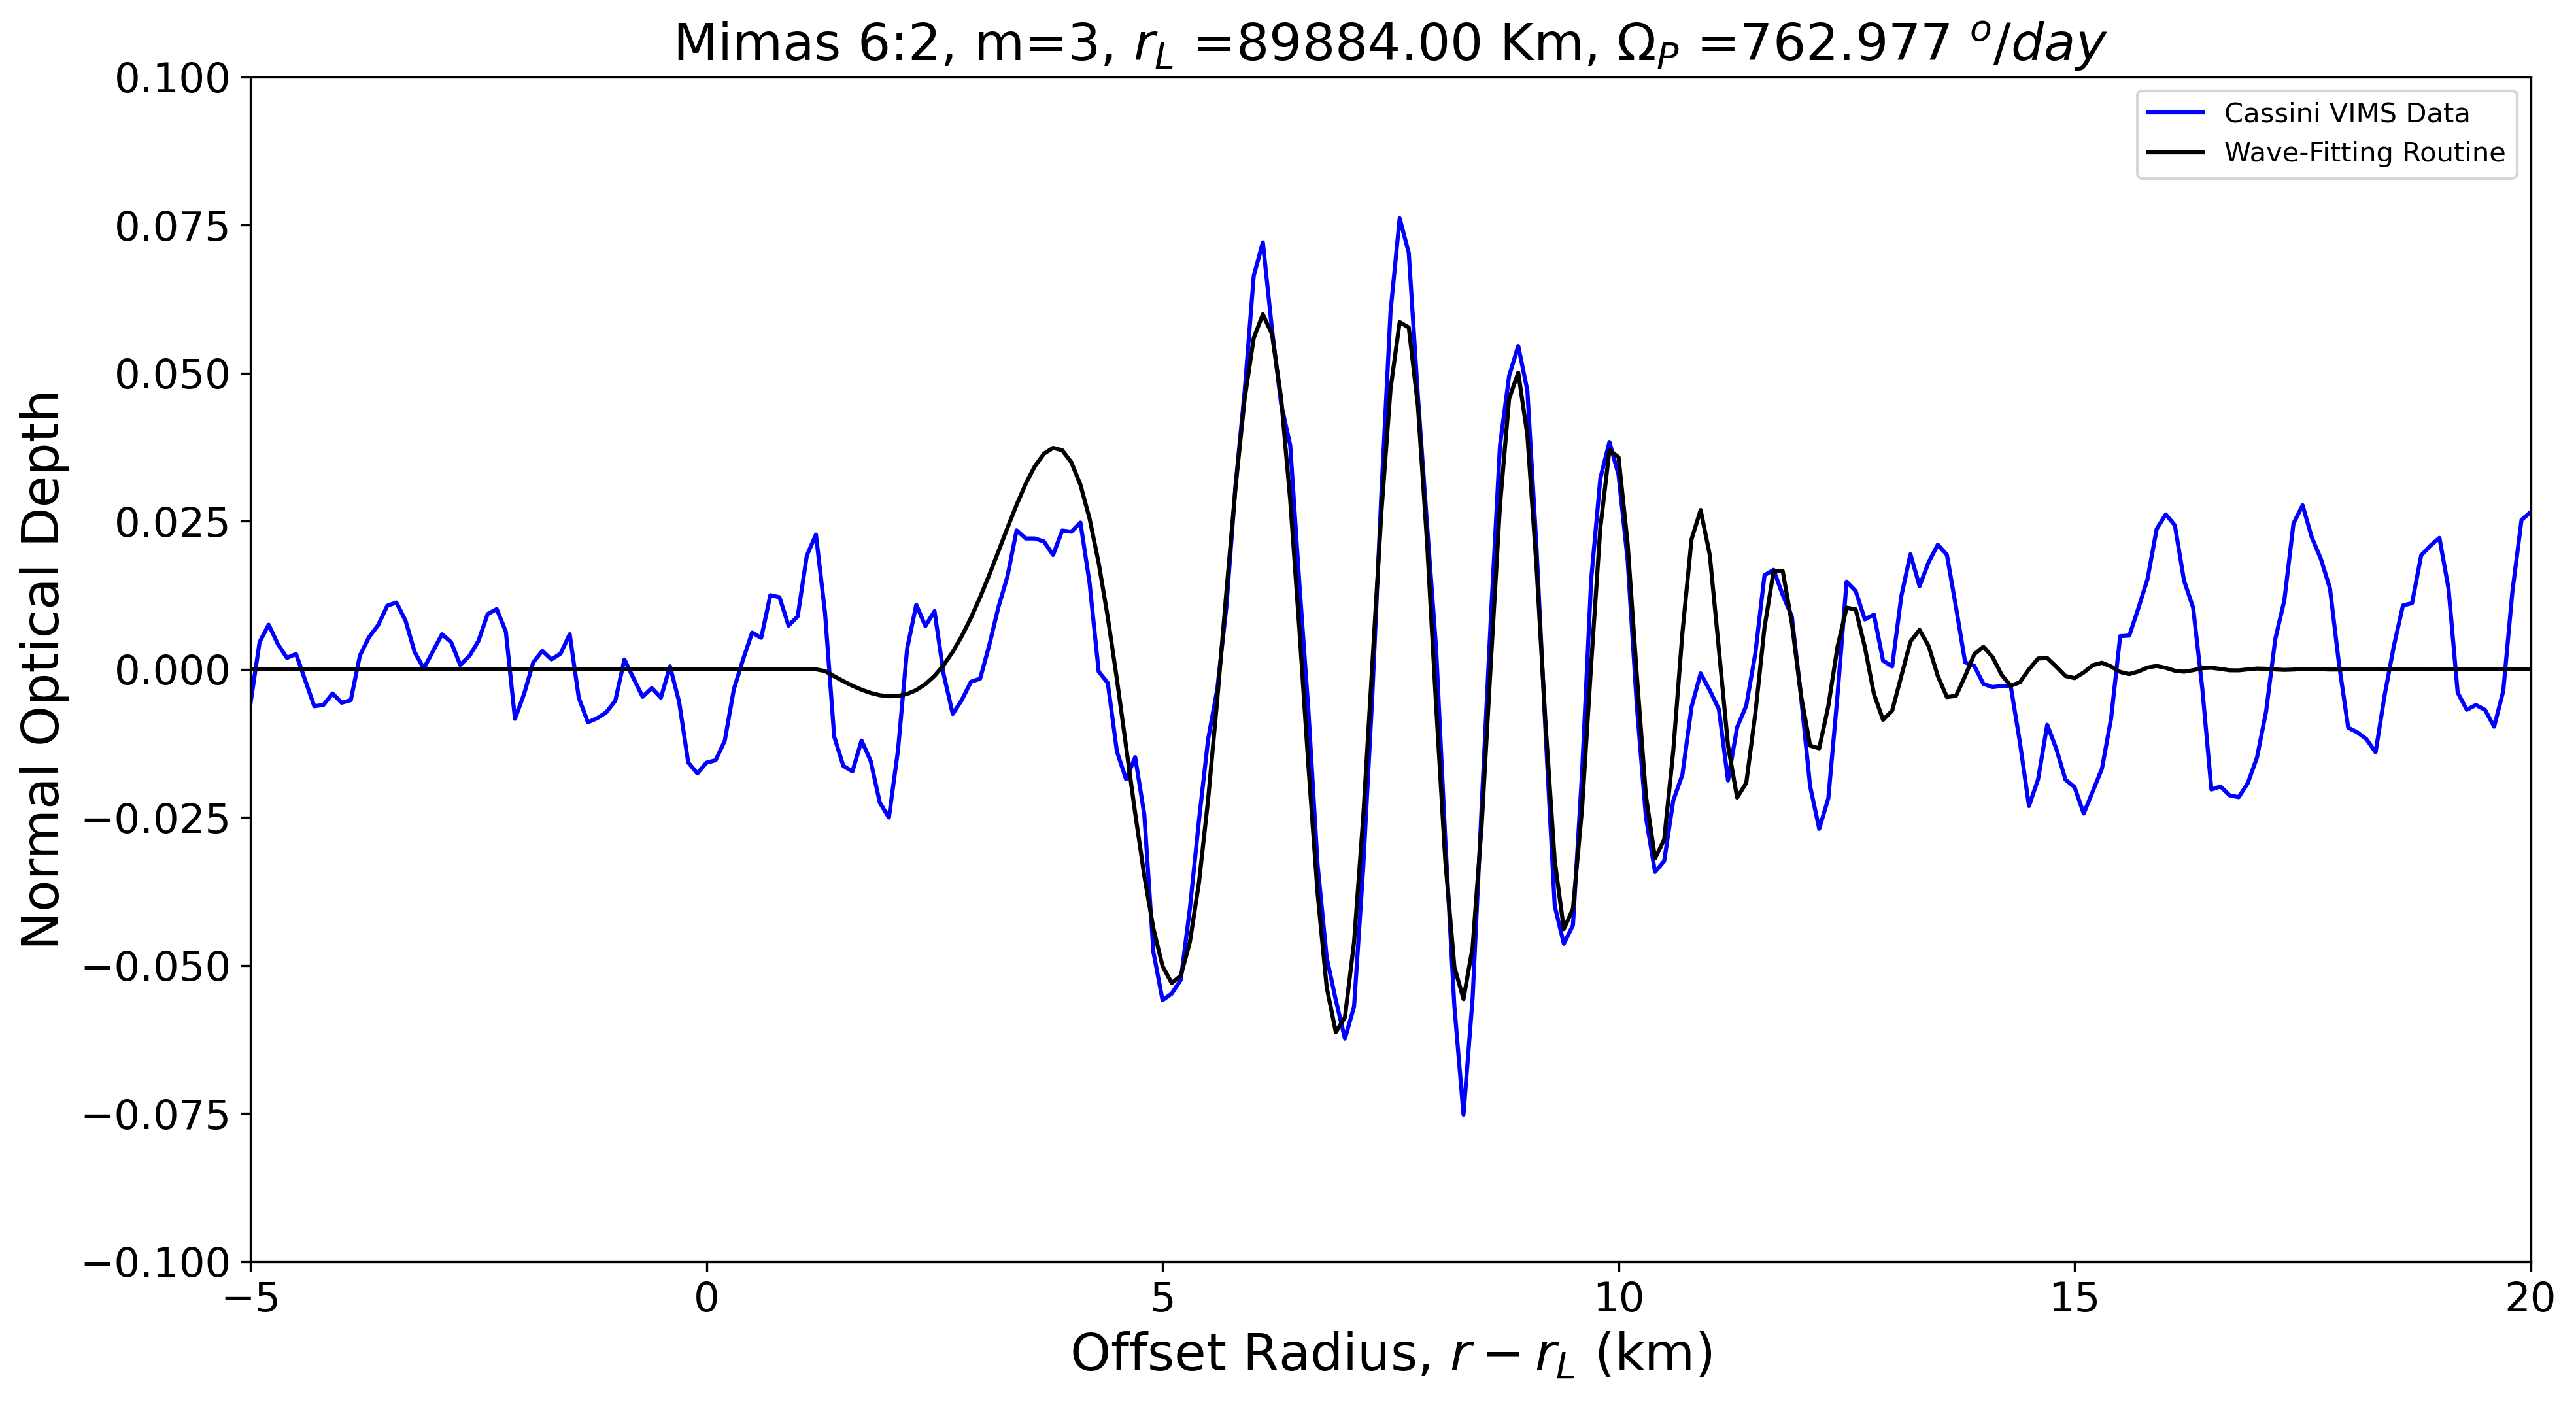
\includegraphics[width=\linewidth]{mimas_62_wavefit.png}
        %\caption{Caption for Mimas62}
        \label{fig:mimas62}
    \end{subfigure}
    \hspace{1\linewidth}

    \begin{subfigure}{0.35\linewidth}
        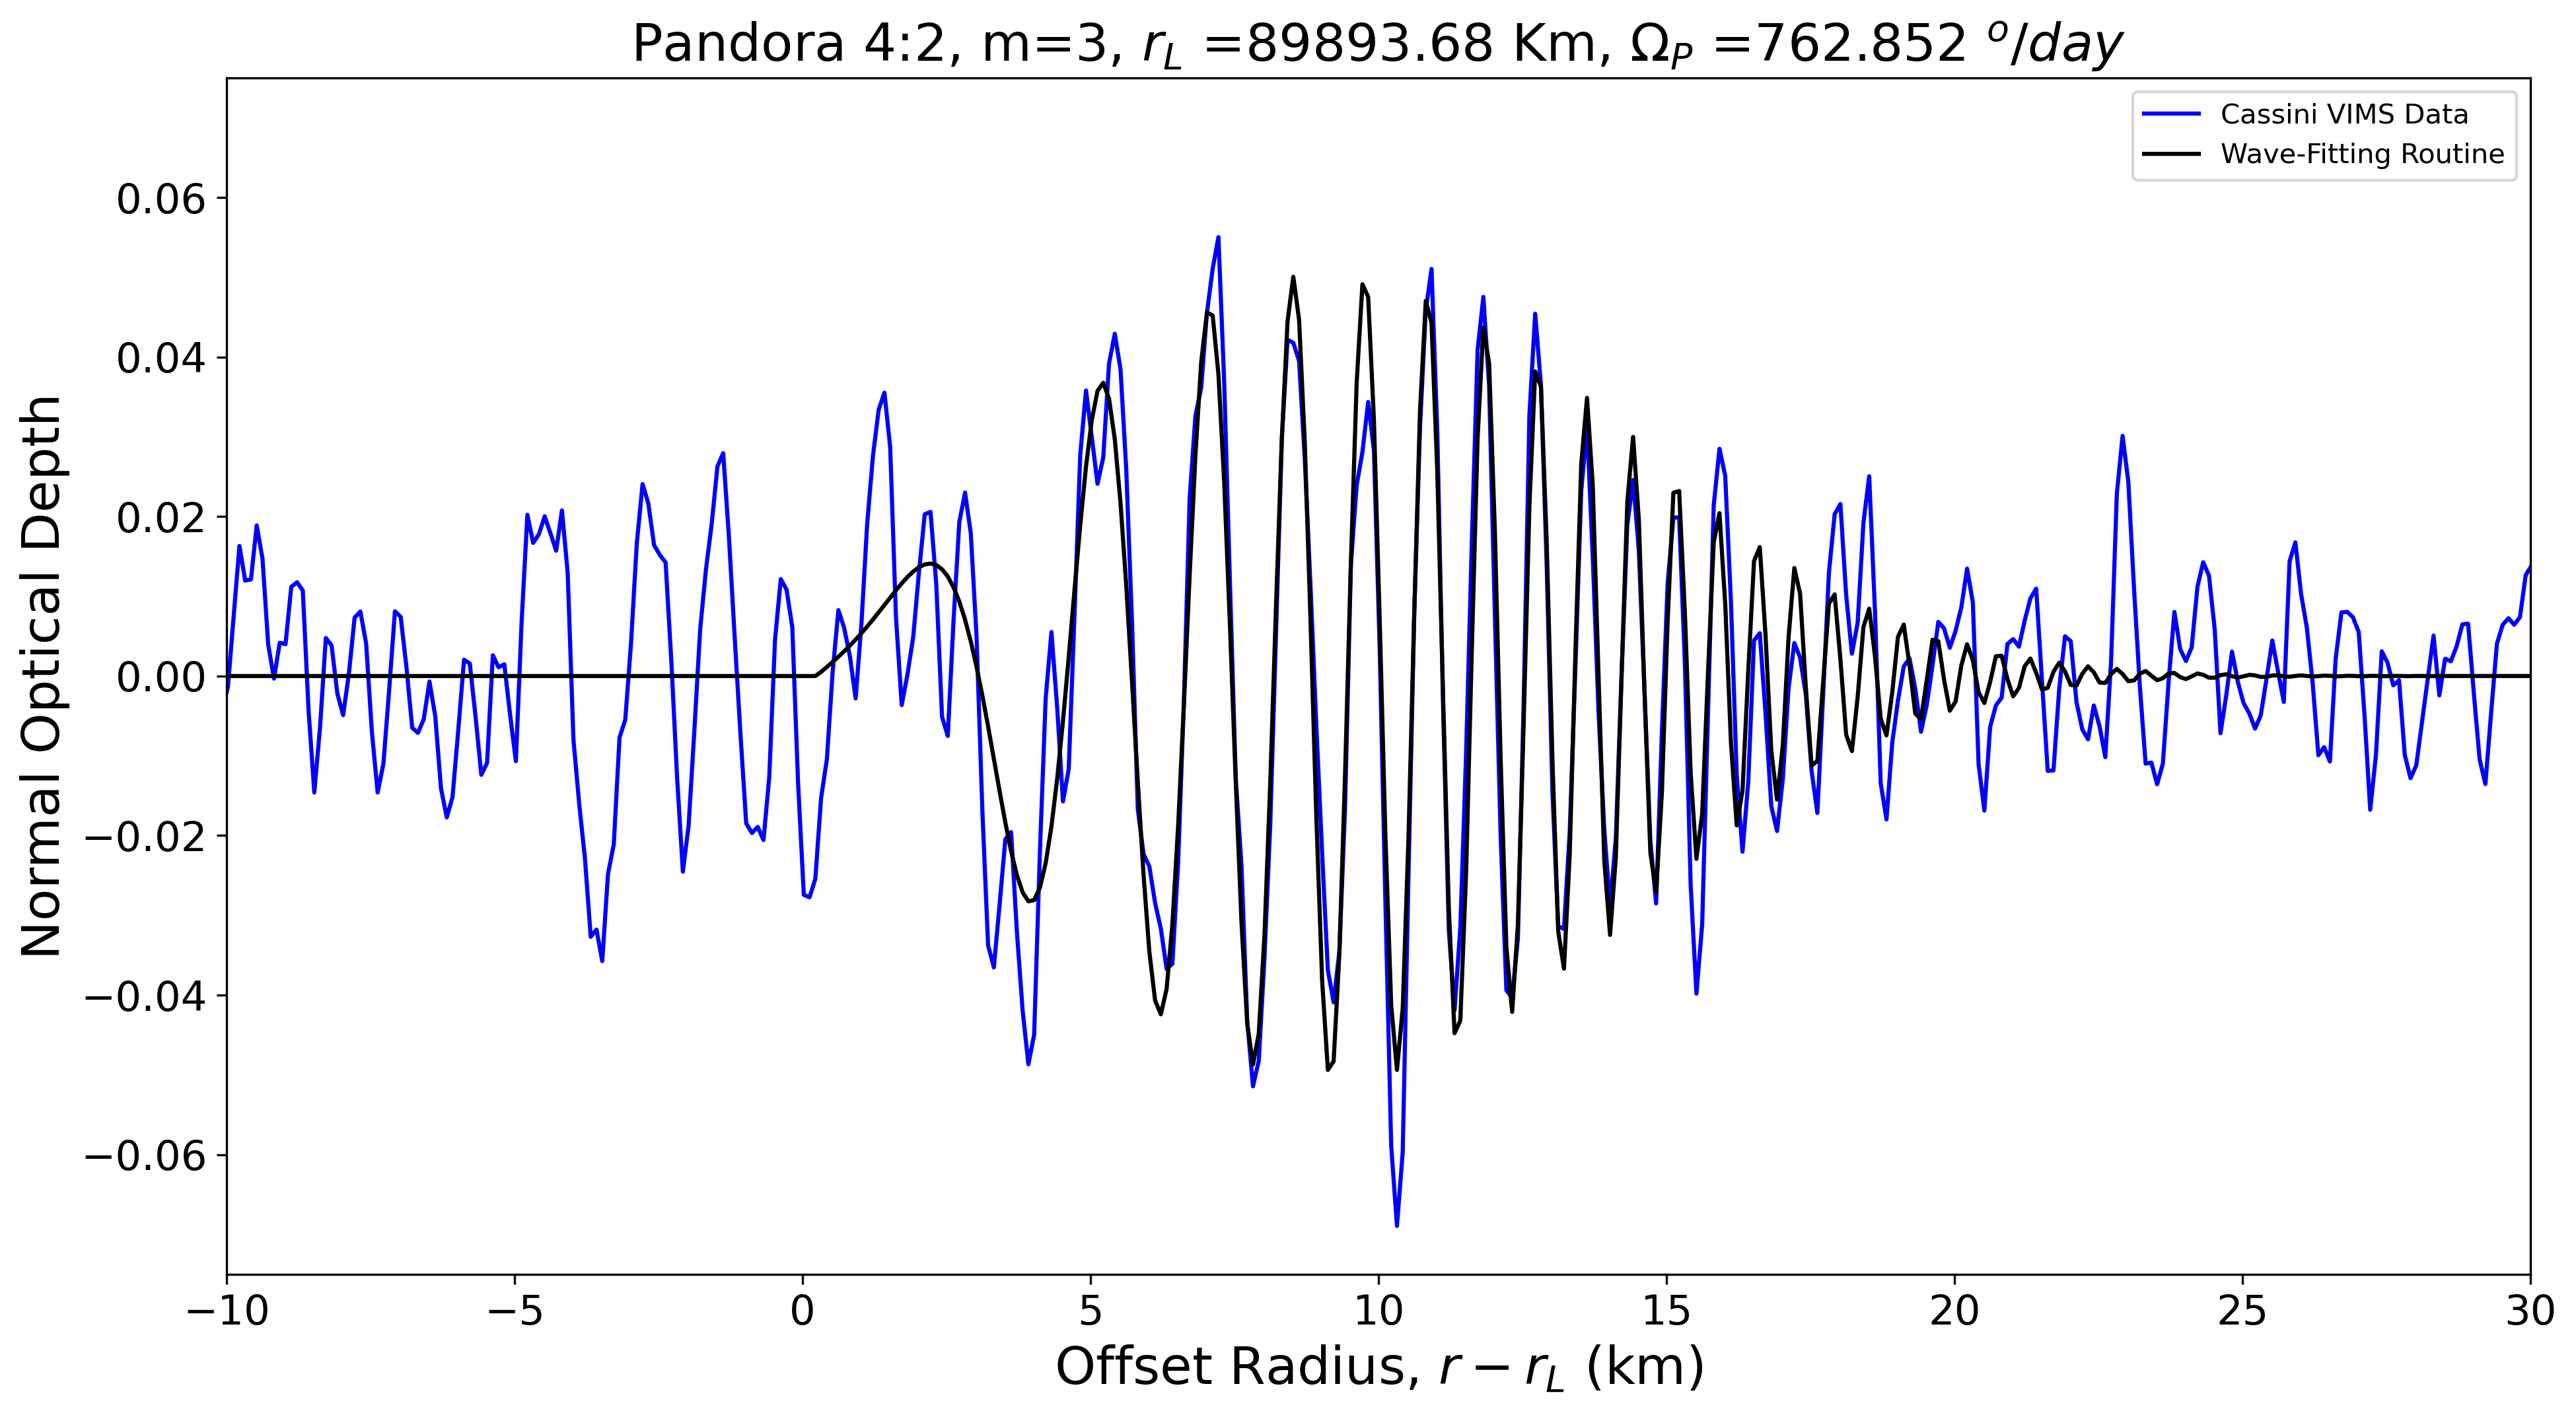
\includegraphics[width=\linewidth]{pandora_42_wavefit.png}
        %\caption{Caption for Pandora42}
        \label{fig:pandora42}
    \end{subfigure}

    \caption{A panel of wave-fitting plots for given Satellite resonances.}
    \label{fig:common-label}
\end{figure}

%............................................................................................................

\begin{table}
\centering
\rotatebox{90}{
%\begin{tabular}{lllll}
\begin{tabular}{|c|c|c|c|c|c|c|c|c|c|}
\hline
\stackon[0pt]{Name}{\stackon[0pt]{Resonance}}& \stackon[0pt]{(Km)}{\stackon[0pt]{Range}{Radial}} &  $m$ & \stackon[0pt]{(Km)}{\stackon[0pt]{Location}{Resonance}}     & \stackon[0pt]{(^{o}/day)}{\stackon[0pt]{Speed}{Pattern}} & a_{fit} (Units) & x_{d} (Units) & \phi_{0} (rad) & x_{r} (Km) & x_{f} (Km) \\
\hline
Mimas 4:1 & 74880 - 74895 & 2 & 74890.07 & 762.988 & 0.2229 \pm 0.0407 & 2.7986 \pm 0.1062 & -4.1870 \pm 0.9080 & 2.6125 \pm 0.6756 & 1.5657 \pm 0.1732 \\
\hline
a & 74880 - 74895 & 2 & 74891.10 & 762.972 & 0.2876 \pm 0.0343 & 2.6310 \pm 0.1137 & -3.4450 \pm 0.6102 & 1.0584 \pm 0.3665 &  1.7589 \pm 0.0518 \\
\hline
Pan 2:1 & 85090 - 85130 & 2 & 85105.02 & 626.032 &  0.0139 \pm 0.0027 &   4.5691 \pm 0.7583 & -6.2832 \pm 1.1633 & 1.1439 \pm 0.3908 & 2.6895 \pm 0.1644 \\
\hline
Atlas 2:1 & 87640 - 87650 & 2 & 87645.68 & 598.312 & 0.1707 \pm 0.0282 & 2.2338 \pm 0.1125 & -0.8399 \pm 0.2801 & 0.3770 \pm 0.1735 & 1.0418 \pm 0.0405 \\
\hline
Prometheus 4:2 & 88420 - 88440 & 3 & 88434.12 & 782.128 & 0.0067 \pm 0.0006 & 5.8369 \pm 0.3091 & 0.2629 \pm 0.4976 &  0.4764 \pm 0.3487 & 1.6954 \pm 0.0611 \\
\hline
b & 89870 - 89890 & 3 & 89883.14 & 762.988 & 0.0102 \pm 0.0015 & 5.7226 \pm 0.2188 &    -3.2372 \pm 0.8792 & 2.7052 \pm 0.1658 & 1.5727 \pm 0.0101 \\
\hline
Mimas 6:2 & 89870 - 89890 & 3 & 89884.00 & 762.977 & 0.0128 \pm 0.0017 &  4.8527 \pm 0.2474 & -1.7461 \pm 0.7624 & 1.2660 \pm 0.2117 & 1.6616 \pm 0.0113 \\
\hline
Pandora 4:2 & 89887 - 89897 & 3 & 89893.68 & 762.852 & 0.0074 \pm 0.0031 & 6.9140 \pm 0.7697 & -3.2364 \pm 0.4213 & 0.2341 \pm 0.2050 & 1.8745 \pm 0.0683 \\
\hline
\end{tabular}
}
\caption{Data for wave-fitting parameters for spiral density waves excited by Saturn's Satellite resonances.}
\end{table}

%...............................................

\subsection{Preliminary Result II}

\subsubsection{Model Computations for Surface Mass Density and Mass Extinction Coefficients: Satellite Resonances}


\begin{table}
\centering
\rotatebox{0}{
%\begin{tabular}{lllll}
\begin{tabular}{|c|c|c|c|c|c|c|c|c|c|}
\hline
\stackon[0pt]{Name}{\stackon[0pt]{Resonance}}& \stackon[0pt]{(Km)}{\stackon[0pt]{Range}{Radial}} &  $m$ & \stackon[0pt]{(Km)}{\stackon[0pt]{Location}{Resonance}} & x_{f} (Km) & \sigma_{0} (Kg m^{-2}) \\
\hline
Mimas 4:1 & 74880 - 74895 & 2 & 74890.07 & 1.5657 \pm 0.1732 & 10.5766 \pm 2.3395 \\
a & 74880 - 74895 & 2 & 74891.10 & 1.7589 \pm 0.0518 & 13.3470 \pm 0.7863 \\
Pan 2:1 & 85090 - 85130 & 2 & 85105.02 & 2.6895 \pm 0.1644 & 18.7122 \pm 2.2876 \\
Atlas 2:1 & 87640 - 87650 & 2 & 87645.68 & 1.0418 \pm 0.0405 & 2.4960 \pm 0.1941 \\
Prometheus 4:2 & 88420 - 88440 & 3 & 88434.12 & 1.6954 \pm 0.0611 &   12.7561 \pm 0.9199 \\
b & 89870 - 89890 & 3 & 89883.14 & 1.5727 \pm 0.0101 & 10.2857 \pm 0.1323 \\
Mimas 6:2 & 89870 - 89890 & 3 & 89884.00 & 1.6616 \pm 0.0113 & 11.4800 \pm 0.1558 \\
Pandora 4:2 & 89887 - 89897 & 3 & 89893.68 & 1.8745 \pm 0.0683 & 14.6055 \pm 1.0637 \\
\hline
\end{tabular}
}
\caption{Surface mass density estimates from theoretical model for spiral density waves excited by Saturn's Satellite resonances.}
\end{table}

%.......................................................................

\begin{figure}
    \centering
    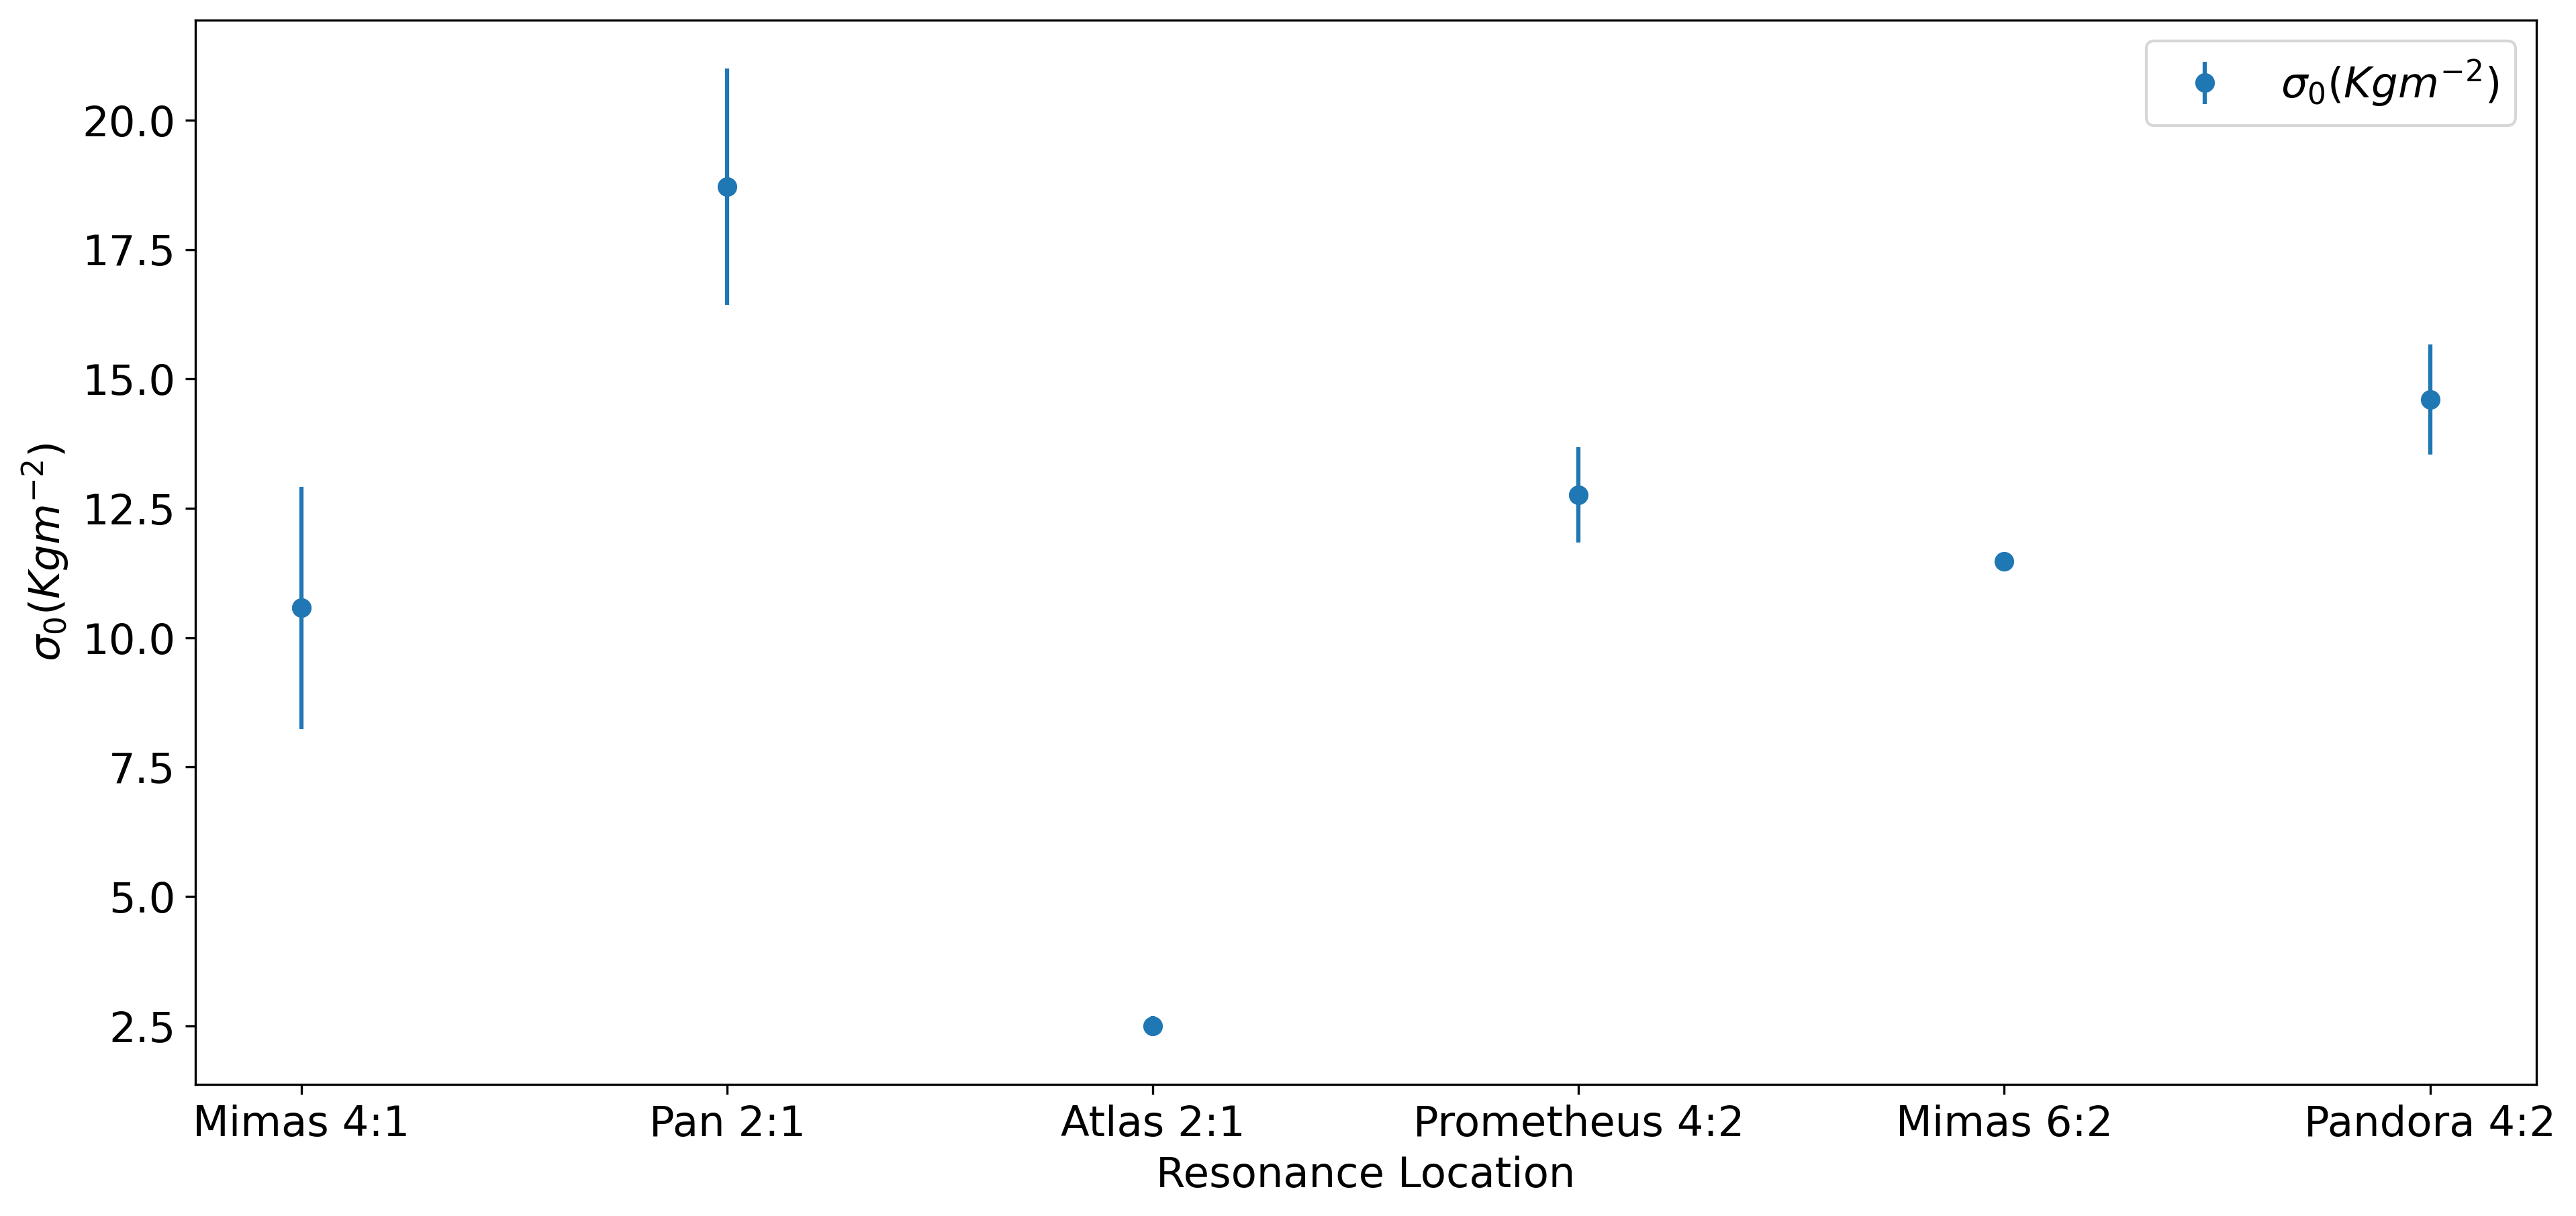
\includegraphics[width=1\linewidth]{Surfacemassdensityplots.png}
    \caption{Scatter plot for Surface mass density estimates for Satellite resonances. Here, we can see the error bars are almost negigible.}
    \label{Surface mass density estimates versus resonance names for Saturn's satellites.}
\end{figure}

%'''''''''''''''''''''''''''''''''''''''''''''''''''''''''''''''''''
\begin{table}
\centering
\rotatebox{0}{
%\begin{tabular}{lllll}
\begin{tabular}{|c|c|c|c|c|c|c|c|c|c|}
\hline
\stackon[0pt]{Name}{\stackon[0pt]{Resonance}}& \stackon[0pt]{(Km)}{\stackon[0pt]{Range}{Radial}} &  $m$ & \stackon[0pt]{(Km)}{\stackon[0pt]{Location}{Resonance}} & \stackon[0pt]{(^{o}/day)}{\stackon[0pt]{Speed}{Pattern}} & \sigma_{0} (Kg m^{-2}) & \tau_{av} & \kappa = \frac{\tau_{av}}{\sigma_{0}} (m^{2}Kg^{-1}) \\
\hline
Mimas 4:1 & 74880 - 74895 & 2 & 74890.07 & 762.988 & 10.5766 \pm 2.3395 & 0.034336 & 0.003246 \pm 0.000718 \\
Pan 2:1 & 85090 - 85130 & 2 & 85105.02 & 626.032 & 18.7122 \pm 2.2876 & 0.082371 & 0.004402 \pm 0.000538 \\
Atlas 2:1 & 87640 - 87650 & 2 & 87645.68 & 598.312 &  2.4960 \pm 0.1941 & 0.061705 & 0.024722 \pm 0.001922 \\
Prometheus 4:2 & 88420 - 88440 & 3 & 88434.12 & 782.128 & 12.7561 \pm 0.9199 & 0.241621 & 0.018942 \pm 0.001366 \\
Mimas 6:2 & 89870 - 89890 & 3 & 89884.00 & 762.977 & 11.4800 \pm 0.1558 & 0.340543 & 0.029664 \pm 0.000403 \\
Pandora 4:2 & 89887 - 89897 & 3 & 89893.68 & 762.852 & 14.6055 \pm 1.0637 & 0.361360 & 0.024741 \pm 0.001801 \\
\hline
\end{tabular}
}
\caption{Mass extinction coefficients estimates from theoretical model for spiral density waves excited by Saturn's Satellite resonances.}
\end{table}

%....................................................................................


\begin{figure}
    \centering
    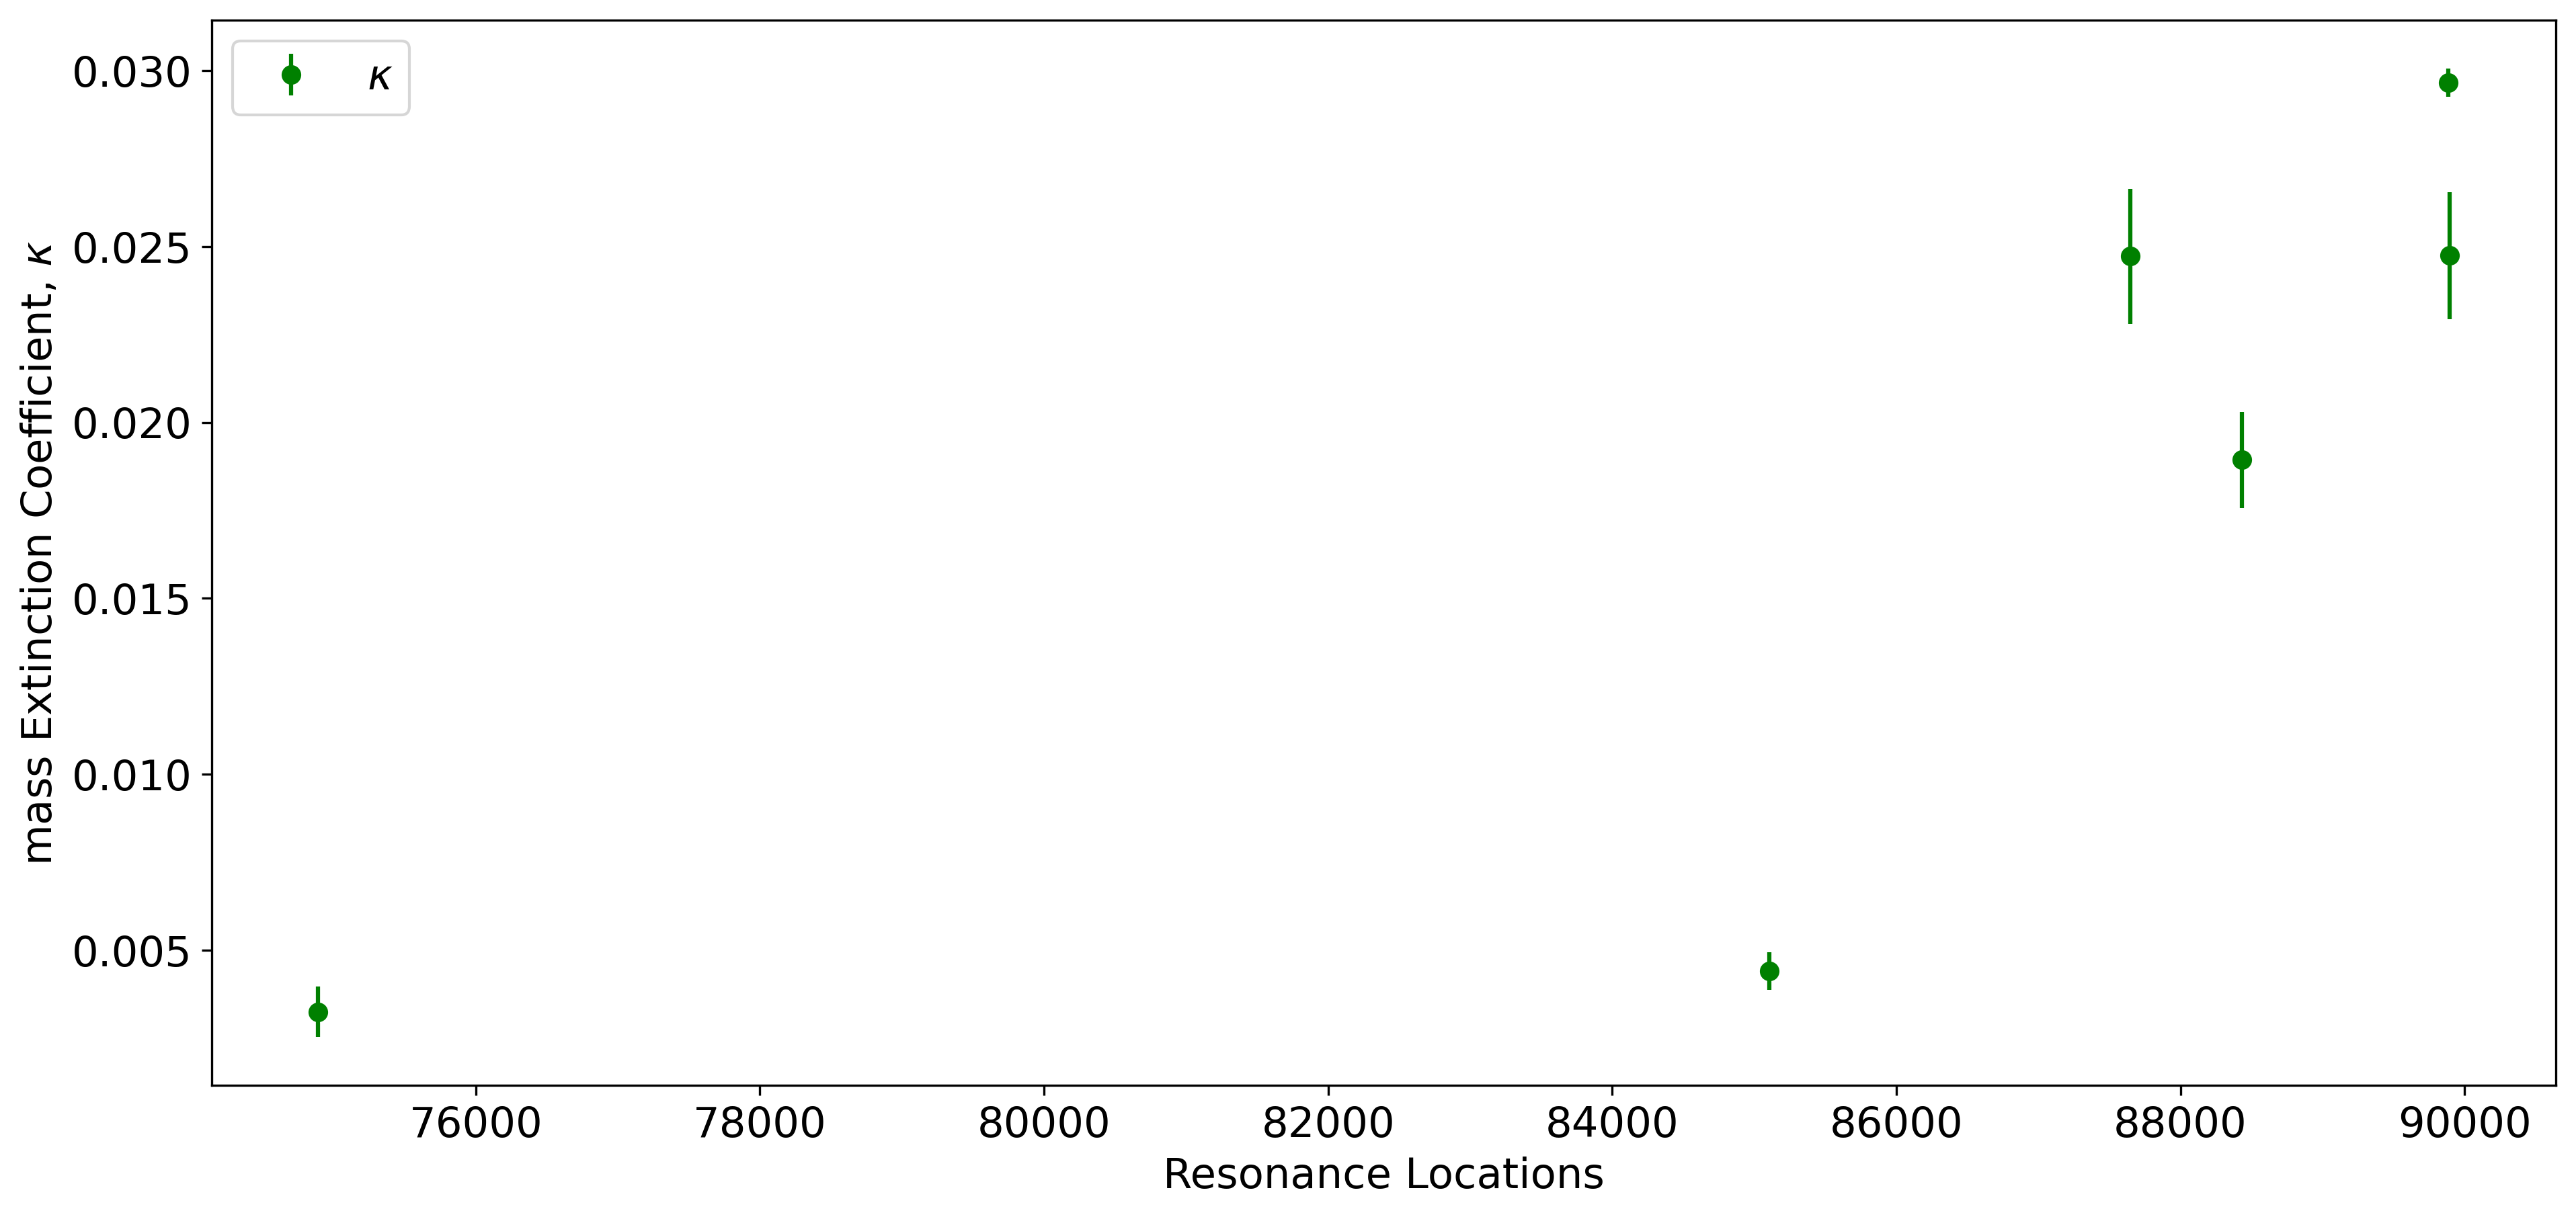
\includegraphics[width=1\linewidth]{satellite_mass_extinction_coefficients.png}
    \caption{Mass extinction coefficients for Satellite Resonances.}
    \label{fig:enter-label}
\end{figure}



%....................................................................................

\begin{table}
\centering
\vspace{0.01pt} % Adjust the value as needed
\rotatebox{90}{
\small
%\begin{tabular}{lllll}
\begin{tabular}{|c|c|c|c|c|c|c|c|c|c|}
\hline
\stackon[0pt]{Name}{\stackon[0pt]{Resonance}} & \stackon[0pt]{(Km)}{\stackon[0pt]{Range}{Radial}} &  $m$ & \stackon[0pt]{(Km)}{\stackon[0pt]{Location}{Resonance}} & \stackon[0pt]{(^{o}/day)}{\stackon[0pt]{Speed}{Pattern}} & \stackon[0pt]{Occultations}{\stackon[0pt]{Faulty}} \\
\hline
Mimas 4:1 & 74880 - 74895 & 2 & 74890.07 & 762.988 & ["RLyr202e","RCas194e"] \\
Pan 2:1 & 85090 - 85130 & 2 & 85105.02 & 626.032 & ["L2Pup206e","betPeg108i","betPeg172i","L2Pup201i","RCas191i", "muCep191i","RSCnc085e","RCas106i"]\\
Atlas 2:1 & 87640 - 87650 & 2 & 87645.68 & 598.312 & ["muCep191i","gamCru094i","RLyr200i"] \\
Prometheus 4:2 & 88420 - 88440 & 3 & 88434.12 & 782.128 &["alpSco245i","RCas106i","VYCMa269i"] \\
Mimas 6:2 & 89870 - 89890 & 3 & 89884.00 & 762.977 &  ["RCas243i","L2Pup199e","RCar191i","betPeg170e","gamCru079i","gamCru073i"]\\
Pandora 4:2 & 89887 - 89897 & 3 & 89893.68 & 762.852 & ["gamCru291i","RCas243i","L2Pup199e","RCar191i","gamCru079i","gamCru073i"]\\

\hline
\end{tabular}
}
\caption{Excluded occultations for spiral density waves excited by Saturn's Satellite resonances.}
\end{table}

%.....................................................................................



%................................................................................

\paragraph{Satellite Waves: Model Computations for Gravitational Potential}


\begin{table}
\centering
\rotatebox{0}{
%\begin{tabular}{lllll}
\begin{tabular}{|c|c|c|c|c|c|c|c|c|c|}
\hline
\stackon[0pt]{Name}{\stackon[0pt]{Resonance}}& \stackon[0pt]{(Km)}{\stackon[0pt]{Range}{Radial}} &  $m$ & \stackon[0pt]{(Km)}{\stackon[0pt]{Location}{Resonance}} & \Psi_{m}^{'} (m^{2}s^{-2}) \\
\hline

Mimas 4:1 & 74880 - 74895 & 2 & 74890.07 & 0.041771 \pm 0.016477 \\
Pan 2:1 & 85090 - 85130 & 2 & 85105.02 & 0.005243 \pm 0.001448 \\
Atlas 2:1 & 87640 - 87650 & 2 & 87645.68 & 0.008836 \pm 0.001821 \\
Prometheus 4:2 & 88420 - 88440 & 3 & 88434.12 & 0.001794 \pm 0.000252 \\
Mimas 6:2 & 89870 - 89890 & 3 & 89884.00 & 0.003120 \pm 0.000419 \\
Pandora 4:2 & 89887 - 89897 & 3 & 89893.68 & 0.002284 \pm 0.000994 \\

\hline
\end{tabular}
}
\caption{Estimates of Gravitational potential from theoretical model for spiral density waves excited by Saturn's Satellite resonances.}
\end{table}



\begin{figure}
    \centering
    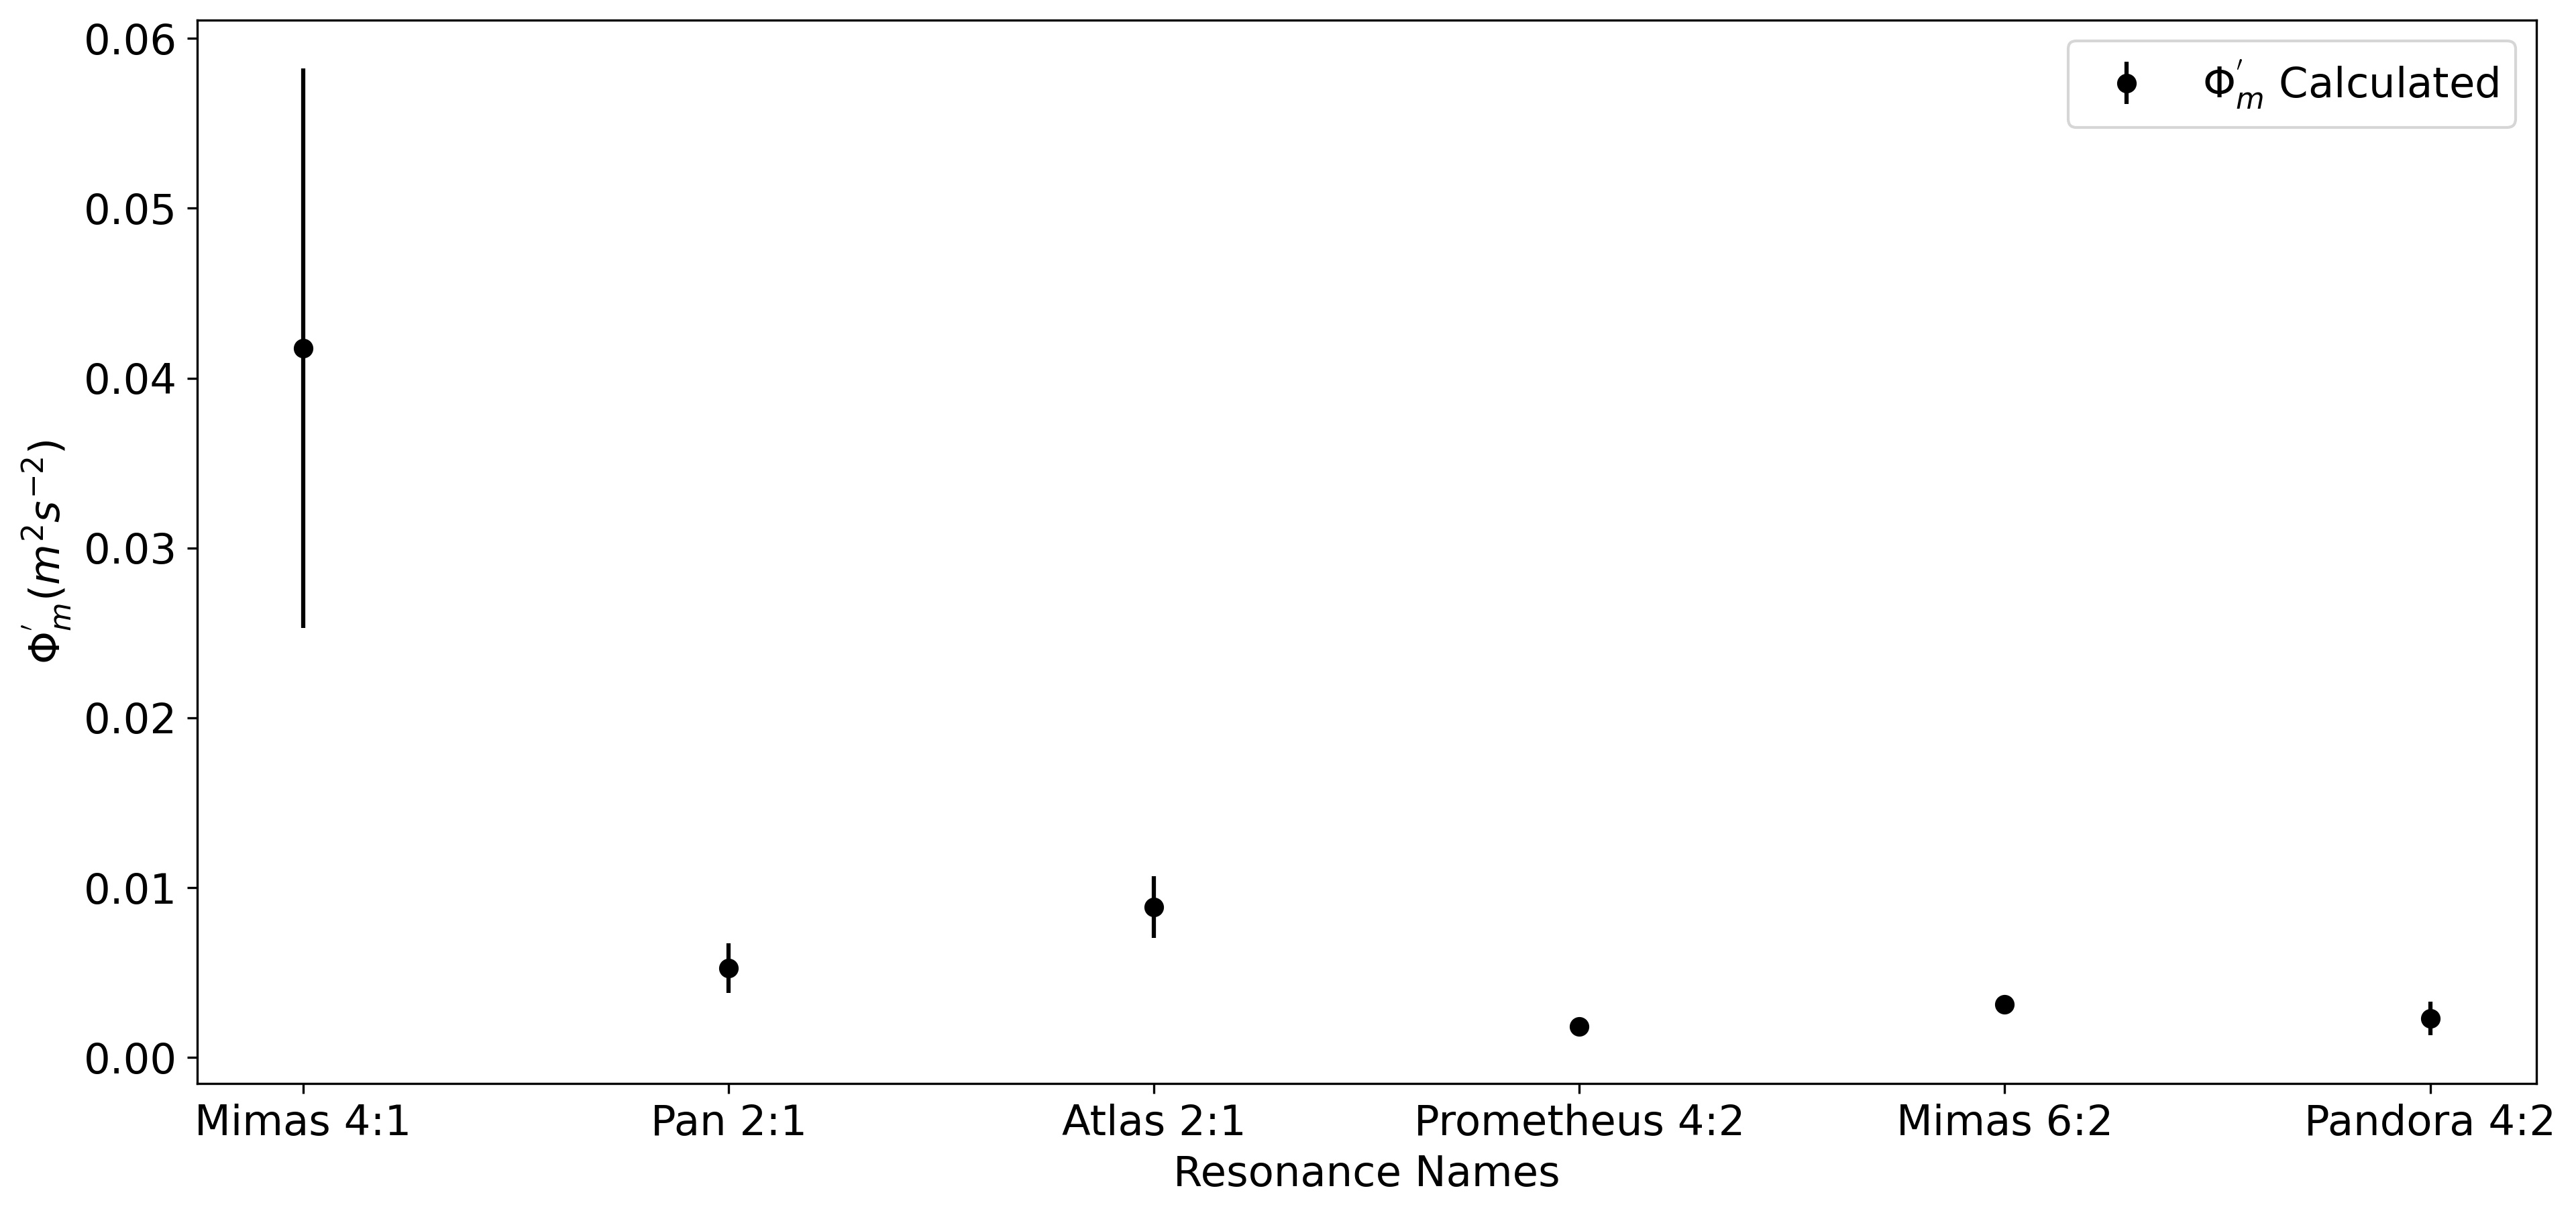
\includegraphics[width=1\linewidth]{satellite_potentialplot_witherrorbars.png}
    \caption{Plot for Calculated Gravitational Potential Values (Satellite waves) with error bars.}
    \label{fig:enter-label}
\end{figure}


\begin{figure}
    \centering
    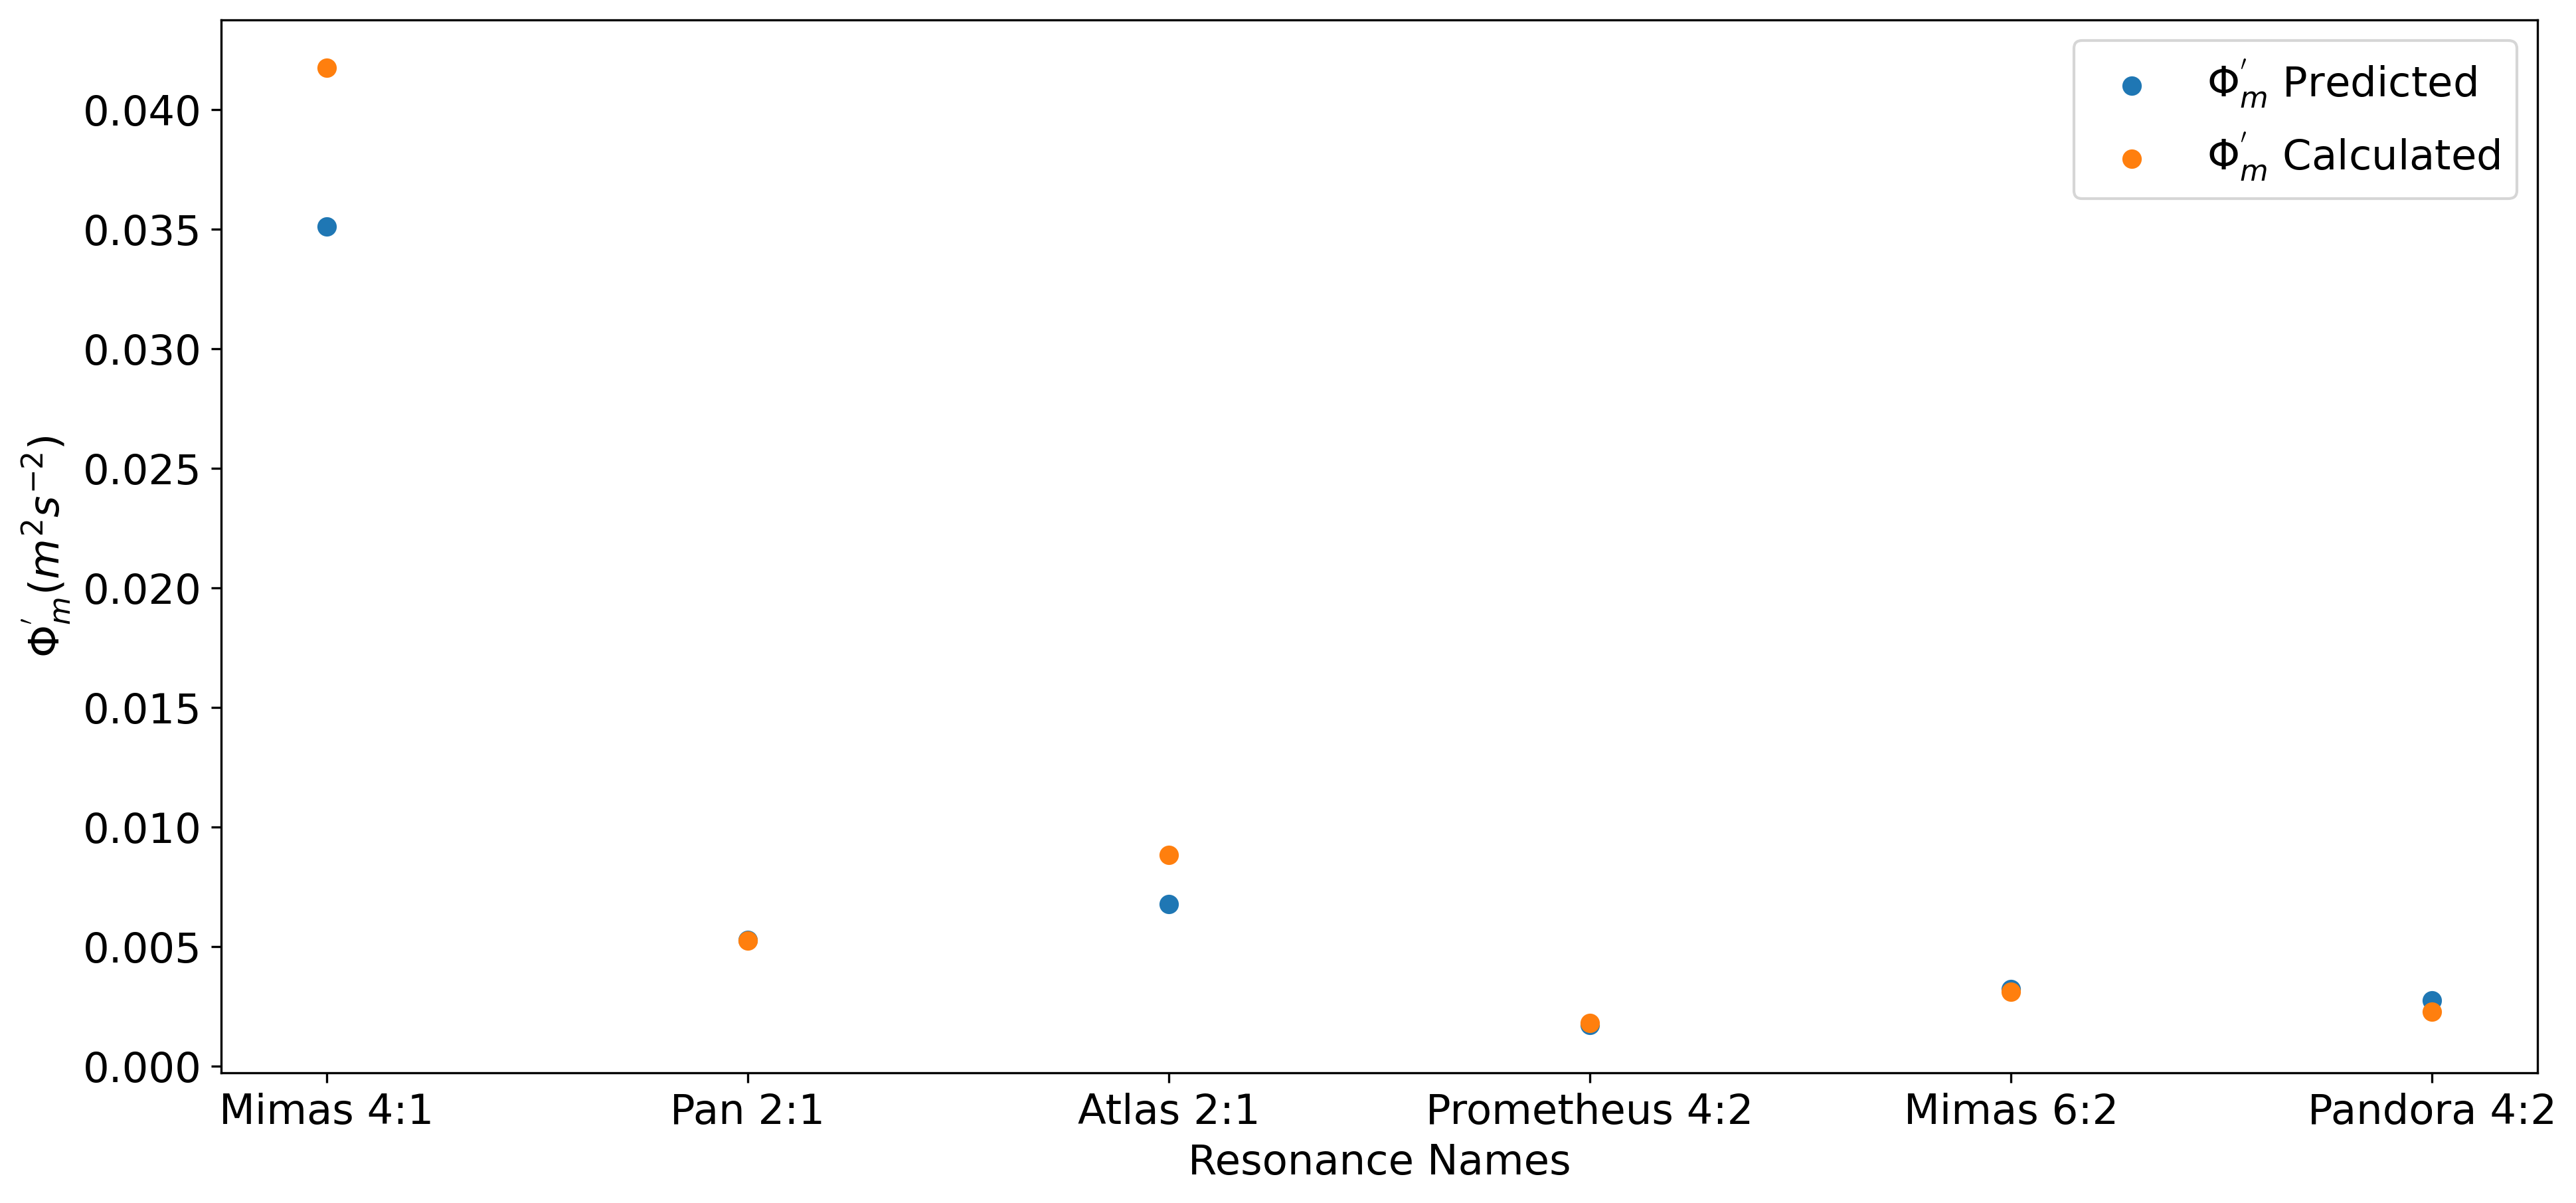
\includegraphics[width=1\linewidth]{predicted_plus_calculated_satellite_potential.png}
    \caption{Scatter Plot for Predicted versus Calculated Gravitational Potential Values (Satellite waves).}
    \label{fig:enter-label}
\end{figure}


\subsubsection{Model Computations for Damping Parameter}

\subsubsection{Model Computations for Viscosity}


%................../////////////////////////......................////////////////////
\section{Preliminary Result III: Applications to non-Satellite Density Waves}

\subsection{Abstract}

\subsection{Introduction}
\subsection{Model Computations for Surface Mass Density and Mass Extinction Coefficients: non-Satellite Resonances}
\subsection{Damping Parameter and Viscosity Estimates: non-Satellite Resonances}
\subsection{Model Computations for Gravitational Potential: non-Satellite Resonances}
\subsection{Computations for Saturn's Planetary Normal-mode Amplitudes:}




%.................................................................................
\section{Discussions}

%.................................................................................

\section{Future Directions}
There is still much to learn about spiral density waves in Saturn's rings, and efficient algorithms for Fourier transforms are an important tool for their analysis. One promising direction for future research is the use of Fourier transforms to study the interaction between spiral waves and other phenomena in the rings, such as resonances with nearby moons. Additionally, new data from the Cassini spacecraft and future missions to Saturn could provide even more detailed information about the structure and dynamics of the rings, opening up new avenues for analysis. To help achieve these objectives, we plan to achieve a more efficient correction factor for our customized algorithm, to help produce efficient and effective results during usage. 

\section{Conclusion}
In conclusion, our study has shed new light on the behavior of waves within Saturn's rings and the factors that influence them. By using efficient Fourier transform algorithms, we were able to quantify the impact of the planet's internal structure on the behavior of these waves. As we continue to uncover new information about Saturn and its rings, these findings will serve as a critical foundation for future research efforts aimed at further exploring the mysteries of our solar system.

\section{Data Availability Statement}
The corresponding authors are committed to promoting open and transparent research practices. They are willing to share the data, models, or codes to facilitate further analysis and validation of the research findings. Collaborators, fellow researchers, and interested parties are encouraged to reach out to the corresponding authors to obtain the requested information. It is important to note that the availability of the data, models, or codes is subject to any applicable legal, ethical, or privacy restrictions. The corresponding authors will ensure that any shared materials comply with relevant regulations and guidelines to protect the privacy and confidentiality of participants or sensitive information. Additionally, the corresponding authors may provide supplementary materials or documentation to enhance the understanding and reproducibility of the research. These additional resources can assist readers in replicating the study or building upon its findings. The corresponding authors can be contacted via their provided contact details or through the designated communication channels outlined in the research publication. They will endeavor to respond to requests in a timely manner, keeping in mind the complexity and scope of the information being requested. Overall, the corresponding authors are dedicated to fostering a culture of collaboration and knowledge sharing, aiming to contribute to the advancement of scientific inquiry and progress.

\section{Acknowledgements}
I gratefully acknowledge the Maker of the Universe, for unending inspiration and momentum to continue in times of greatest need. I also appreciate Prof. Matthew Hedman and other esteemed co-authors for helpful comments, suggestions and contributions. This research has made use of data obtained from the recent Cassini Mission (2004-2017), as well as softwares from Python libraries. 




%.................................................................................


%................................................................................


\bibliographystyle{plain}\bibliography{reference}

\end{document}


%This study explores the possibility that Saturn's rings function as seismographs, recording gravitational signals resulting from the acoustic oscillation modes of the planet. Certain spiral density waves in Saturn's rings are generated through resonances with planetary normal modes, making them valuable probes of Saturn's internal structure. Previous research has primarily focused on the rotation rates of these waves, which yield precise measurements of Saturn's oscillation frequencies. However, other characteristics of these waves also contain valuable information about the planet's interior. In this work, we have investigated the amplitudes of the ring waves by analyzing high signal-to-noise profiles obtained from Cassini's Visual and Infrared Mapping Spectrometer (VIMS) occultations. By fitting these profiles, we have successfully determined the amplitudes of the perturbing potentials responsible for generating numerous waves. Furthermore, we have estimated the corresponding non-zonal gravitational spherical harmonic coefficients that generate approximately a dozen of these spiral density waves. The observed spectrum primarily consists of the fundamental mode (f-mode) oscillations with relatively low spherical harmonic degrees. Analyzing these oscillations provides insights into the excitation mechanisms of such oscillations within Saturn's interior. By combining these findings with the precise measurements of oscillation frequencies from the rotation rates, we can gain a comprehensive understanding of Saturn's internal structure and dynamics.

%Keywords: Saturn, rings, seismographs, acoustic oscillation modes, spiral density waves, planetary normal modes, oscillation frequencies, spherical harmonic coefficients, Cassini, VIMS, occultations, internal structure, f-mode oscillations.